\RequirePackage{silence} % :-\
    \WarningFilter{scrreprt}{Usage of package `titlesec'}
    %\WarningFilter{scrreprt}{Activating an ugly workaround}
    \WarningFilter{titlesec}{Non standard sectioning command detected}
\documentclass[%twoside,openright, 
                parts=false,titlepage,numbers=noenddot,%1headlines,
                headinclude,footinclude,%cleardoublepage=empty,
                abstract=on,
                BCOR=5mm,paper=b5,fontsize=11pt,dvipsnames,openany,captions=tableabove,
                ]{scrbook}

% python terminal: 
% import os, shutil;new='jakob_daniel_18409686_MEEN30020_2020-21_assign1_report.pdf';os.replace(r'main.pdf',new); newPath = shutil.copy(new, '../')
%\includeonly{frontbackmatter/Contents.tex, frontbackmatter/Acknowledgments.tex, frontbackmatter/Abstract.tex, chapters/Chapter02.tex}


% latexmk -lualatex -auxdir=".aux" -shell-escape -recorder-  main.tex
% lualatex  -shell-escape -aux-directory=".aux"  "main.tex"
% makeindex -s nomencl.ist -t "main.nlg" -o "main.nls" ".aux/main.nlo"
% biber  ".aux/main.bcf"

%********************************************************************
% Note: Make all your adjustments in here
%*******************************************************
% ****************************************************************************************************
% classicthesis-config.tex
% formerly known as loadpackages.sty, classicthesis-ldpkg.sty, and classicthesis-preamble.sty
% Use it at the beginning of your ClassicThesis.tex, or as a LaTeX Preamble
% in your ClassicThesis.{tex,lyx} with % ****************************************************************************************************
% classicthesis-config.tex
% formerly known as loadpackages.sty, classicthesis-ldpkg.sty, and classicthesis-preamble.sty
% Use it at the beginning of your ClassicThesis.tex, or as a LaTeX Preamble
% in your ClassicThesis.{tex,lyx} with % ****************************************************************************************************
% classicthesis-config.tex
% formerly known as loadpackages.sty, classicthesis-ldpkg.sty, and classicthesis-preamble.sty
% Use it at the beginning of your ClassicThesis.tex, or as a LaTeX Preamble
% in your ClassicThesis.{tex,lyx} with \input{classicthesis-config}
% ****************************************************************************************************
% If you like the classicthesis, then I would appreciate a postcard.
% My address can be found in the file ClassicThesis.pdf. A collection
% of the postcards I received so far is available online at
% http://postcards.miede.de
% ****************************************************************************************************


% ****************************************************************************************************
% 0. Set the encoding of your files. UTF-8 is the only sensible encoding nowadays. If you can't read
% äöüßáéçèê∂åëæƒÏ€ then change the encoding setting in your editor, not the line below. If your editor
% does not support utf8 use another editor!
% ****************************************************************************************************
\usepackage[utf8]{inputenc}
\usepackage[T1]{fontenc} % T2A for cyrillics

\usepackage[british]{babel}
\usepackage{setspace}
\usepackage[british]{datetime2} % Edit \today date display
\DTMlangsetup[en-GB]{ord=raise}

% ****************************************************************************************************
% 1. Personal data and user ad-hoc commands (insert your own data here)
% ****************************************************************************************************
\newcommand{\myTitle}{Optimising the Hybrid Operation Temperature Window of a Hybrid Heating System in the Irish Climate\xspace}
\newcommand{\mySubtitle}{A Numerical Simulation Study of an Air-Water Heat Pump and Conventional Gas Boiler in a Residential Setting\xspace}
\newcommand{\myDegree}{Mechanical Engineering Master's (MEng.)\xspace}
\newcommand{\myName}{Daniel Jakob\xspace}
\newcommand{\myStdNumber}{18409686}
\newcommand{\myProf}{Prof. Donal Finn\xspace}
\newcommand{\HoS}{Prof. Kenneth Stanton\xspace}
%\newcommand{\myOtherProf}{hmm\xspace}
%\newcommand{\mySupervisor}{Prof. Donal Finn\xspace}
\newcommand{\myCollaborator}{Dr Mohammad Saffari\xspace}
\newcommand{\myExaminer}{Dr Joe Bloggs\xspace}
\newcommand{\myFaculty}{College of Engineering \& Architecture\xspace}
\newcommand{\myDepartment}{School of Mechanical and Materials Engineering\xspace}
\newcommand{\myUni}{University College Dublin\xspace}
\newcommand{\myLocation}{Belfield, Dublin 4\xspace}
\newcommand{\myCountry}{Ireland\xspace}
\newcommand{\myPrintLocation}{Ballsbridge, Dublin 4, Ireland}
%\newcommand{\myTime}{August 2022\xspace}
\newcommand{\myVersion}{v0.1}
\newcommand{\ctVersion}{\classicthesis}
\newcommand{\mykeywords}{Hybrid heat pumps}
\newcommand{\mysubject}{A numerical simulation study of an air-water heat pump and conventional gas boiler hybrid heating system in the Irish climate to optimize the bivalent temperature.}

\DTMsavedate{submitdate}{2023-05-22}
\DTMsavedate{duedate}{2024-11-10}
\DTMsavedate{printdate}{2023-05-15}



% ********************************************************************
% Setup, finetuning, and useful commands
% ********************************************************************
\providecommand{\mLyX}{L\kern-.1667em\lower.25em\hbox{Y}\kern-.125emX\@}
\newcommand{\ie}{i.\,e.,}
\newcommand{\Ie}{I.\,e.,}
\newcommand{\eg}{e.\,g.,}
\newcommand{\Eg}{E.\,g.,}
\newcommand{\modelica}{\texttt{Modelica}\xspace}
\newcommand{\HP}{\ac{HP}\xspace}
\newcommand{\HPs}{\acp{HP}\xspace}
\newcommand{\ASHP}{\ac{ASHP}\xspace}
\newcommand{\ASHPs}{\ac{ASHPs}\xspace}
\newcommand{\AWHP}{\ac{AWHP}\xspace}
\newcommand{\AWHPs}{\acp{AWHP}\xspace}

% ****************************************************************************************************


% ****************************************************************************************************
% 2. Loading some handy packages
% ****************************************************************************************************
% ********************************************************************
% Packages with options that might require adjustments
% ********************************************************************
% Spanish languages need extra options in order to work with this template
%\PassOptionsToPackage{spanish,es-lcroman}{babel}

\usepackage{parskip} % paragraph skips instead of indents 
%\setlength{\parindent}{0em}
%\setlength{\parskip}{1em} 

\usepackage{csquotes}
\usepackage[  
backend=biber,bibencoding=utf8, %instead of bibtex
%backend=bibtex8,bibencoding=ascii,%
language=english,%
style=numeric-comp,%
%style=authoryear-comp, % Author 1999, 2010
%bibstyle=authoryear,dashed=false, % dashed: substitute rep. author with ---
%sorting=nyt, % name, year, title
sorting=none, % sort by appearance
maxbibnames=10, % default: 3, et al.
maxcitenames = 5,
backref=true,%
natbib=true % natbib compatibility mode (\citep and \citet still work)
]{biblatex}

% Places bib numeric in left margin 
\defbibenvironment{bibliography}
{\list{\printtext[labelnumberwidth]{%
    \printfield{prefixnumber}%
    \printfield{labelnumber}}}
{\setlength{\bibhang}{0pt}%
\setlength{\leftmargin}{\bibhang}%
\setlength{\itemindent}{-\leftmargin}%
\setlength{\itemsep}{\bibitemsep}%
\setlength{\parsep}{\bibparsep}}}
{\endlist}
{\item}

\AtEveryBibitem{ % clears URL date
    \clearfield{urldate}
    \clearfield{urlyear}
    \clearfield{urlmonth}
}
\renewcommand{\bibpagerefpunct}{\addperiod\space}
\DefineBibliographyStrings{english}{
  backrefpage={\!\!},
  backrefpages={\!\!}
}


\RequirePackage{mathtools} % Required for some maths elements 
\usepackage{amsmath, amsthm,amssymb} % math environments and more by the AMS


%\RequirePackage{url} % allows websites to be referenced

\usepackage[htt]{hyphenat}
 

% ********************************************************************
% General useful packages
% ********************************************************************
\usepackage{graphicx} %
\graphicspath{{figures/}}
\usepackage{scrhack} % fix warnings when using KOMA with listings package
\usepackage{xspace} % to get the spacing after macros right
\RequirePackage[printonlyused,smaller]{acronym} % nice macros for handling all acronyms in the thesis
%\renewcommand{\bflabel}[1]{{#1}\hfill} % fix the list of acronyms --> no longer working
%\renewcommand*{\acpfont}[1]{\textsc{#1}}
%\renewcommand*{\aclabelfont}[1]{\acpfont{#1}}
%\def\bflabel#1{{#1\hfill}}
%\def\bflabel#1{{\acpfont{#1}\hfill}}
%\def\aclabelfont#1{\acpfont{#1}}

\usepackage{import}

\usepackage{enumitem}
\renewcommand{\theenumi}{\arabic{enumi}.}
\renewcommand{\labelenumi}{\theenumi}
\renewcommand{\theenumii}{(\alph{enumii})}
\renewcommand{\labelenumii}{\theenumii}
\renewcommand{\theenumiii}{\roman{enumiii}.}
\renewcommand{\labelenumiii}{\theenumiii}
\renewcommand{\theenumiv}{\Alph{enumiv}.}
\renewcommand{\labelenumiv}{\theenumiv}

\usepackage[tight-spacing=true]{siunitx}

\usepackage{multirow}

\usepackage{nomencl}
\makenomenclature
%% This will add the subgroups
%----------------------------------------------
\usepackage{etoolbox}
\renewcommand\nomgroup[1]{%
  \item[\bfseries
  \ifstrequal{#1}{A}{Physics Constants}{%
  \ifstrequal{#1}{B}{Subscripts}{%
  \ifstrequal{#1}{C}{Other Symbols}{}}}%
]}
%----------------------------------------------

%% This will add the units
%----------------------------------------------
\newcommand{\nomunit}[1]{%
\renewcommand{\nomentryend}{\hspace*{\fill}#1}}
%----------------------------------------------

% ****************************************************************************************************
%\usepackage{pgfplots} % External TikZ/PGF support (thanks to Andreas Nautsch)
%\usetikzlibrary{external}
% \tikzexternalize[prefix=tikzexternalize/,optimize command away=\includepdf]
% \makeatletter
%     \tikzset{%
%         external/system call={%
%             lualatex %
%                 \tikzexternalcheckshellescape %
%                 -halt-on-error %
%                 -interaction=batchmode %
%                 -output-directory=".aux" %
%                 -jobname "\image" %
%                 "\texsource"%
%         },
%         /pgf/images/include external/.code={%
%             \includegraphics{.aux/#1}%
%         },%
%     }
% \makeatother
% ****************************************************************************************************

\usepackage[flushleft]{threeparttable} % table notes

% Need to use MATLAB2TikZ %%% 
\usepackage{pgfplots}

% \usepgfplotslibrary{patchplots}
% \usepackage{grffile}
\usetikzlibrary{arrows,
                  calc,
                  intersections,
                  fit,
                  shapes.geometric,
                  positioning,
                  angles, 
                  quotes,
                  plotmarks, 
                  arrows.meta}
% \usepackage{tikz-3dplot}


\usepackage{pgfplotstable}
\pgfplotsset{compat=1.18, 
        colormap={mycolor}{
        rgb255=(0, 181, 26)
        rgb255=(255,255,0)
        rgb255=(255, 45, 33)
    },
    }
\usepackage{diagbox}
\usepackage{colortbl}
\usepackage{tikzscale}
% \pgfplotstableset{% global config, for example in the preamble
% empty cells with={--}, % replace empty cells with '--'
% every head row/.style={before row=\toprule,after row=\midrule},
% every last row/.style={after row=\bottomrule}
% }

%\pgfkeys{/pgf/plot/gnuplot call={cd .aux && gnuplot}}

\pgfplotstableset{
    /color cells/min/.initial=1000,
    /color cells/max/.initial=8000,
    /color cells/textcolor/.initial=,
    %
    % Usage: 'color cells={min=<value which is mapped to lowest color>, 
    %   max = <value which is mapped to largest>}
    color cells/.code=
    {%
        \pgfqkeys{/color cells}{#1}%
        \pgfkeysalso
        {%
            postproc cell content/.code=
            {%
                \begingroup
                \pgfkeysgetvalue{/pgfplots/table/@preprocessed cell content}\value
                \pgfmathfloatparsenumber{\value}%
                \pgfmathfloattofixed{\pgfmathresult}%
                \let\value=\pgfmathresult
                \pgfplotscolormapaccess
                    [\pgfkeysvalueof{/color cells/min}:\pgfkeysvalueof{/color cells/max}]
                    {\value}
                    {\pgfkeysvalueof{/pgfplots/colormap name}}
                \pgfkeysgetvalue{/pgfplots/table/@cell content}\typesetvalue %This is the important if-statement for font color selection
                \ifdim\value pt<.5pt\relax
                  \def\textcolorvalue{black}%
                \else
                  \def\textcolorvalue{black}%
                \fi
                \toks0=\expandafter{\typesetvalue}%
                \xdef\temp{%
                    \noexpand\pgfkeysalso{%
                        @cell content={%
                            \noexpand\cellcolor[rgb]{\pgfmathresult}%
                            \noexpand\definecolor{mapped color}{rgb}{\pgfmathresult}%
                            \ifx\textcolorvalue\empty
                            \else
                                \noexpand\color{\textcolorvalue}%
                            \fi
                            \the\toks0 %
                        }%
                    }%
                }%
                \endgroup
                \temp
            }%
        }%
    }%
}

\usepackage[ruled,vlined]{algorithm2e}


% ****************************************************************************************************
% 3. Setup floats: tables, (sub)figures, and captions
% ****************************************************************************************************
\usepackage{tabularx} % better tables
  \setlength{\extrarowheight}{3pt} % increase table row height
\newcommand{\tableheadline}[1]{\multicolumn{1}{l}{\spacedlowsmallcaps{#1}}}
\newcommand{\myfloatalign}{\centering} % to be used with each float for alignment
%\usepackage{subfig}
\usepackage[labelformat=simple]{subcaption}

%\usepackage{multirow} % to have multirow cells in tables

% ****************************************************************************************************


\appto{\appendix}{ % Makes tables, listing, figures etc appear lowercase.
\renewcommand\thefigure{\spacedlowsmallcaps{\thechapter}.\arabic{figure}}
\renewcommand\theequation{\spacedlowsmallcaps{\thechapter}.\arabic{equation}}
%\renewcommand{\thelstlisting}{\spacedlowsmallcaps{\thechapter}.\arabic{lstlisting}}
\renewcommand\thetable{\spacedlowsmallcaps{\thechapter}.\arabic{table}}
}

\DeclareSIUnit{\kWh}{kWh}
\DeclareSIUnit{\EUR}{\text{\euro}}
% ****************************************************************************************************
% 4. Setup code listings
% ****************************************************************************************************
%\usepackage{listings}
%\lstset{emph={trueIndex,root},emphstyle=\color{BlueViolet}}%\underbar} % for special keywords
% \lstset{language=[LaTeX]Tex,%C++,
%   morekeywords={PassOptionsToPackage,selectlanguage},
%   keywordstyle=\color{RoyalBlue},%\bfseries,
%   basicstyle=\small\ttfamily,
%   %identifierstyle=\color{NavyBlue},
%   commentstyle=\color{Green}\ttfamily,
%   stringstyle=\rmfamily,
%   numbers=left,%none
%   numberstyle=\scriptsize,%\tiny
%   stepnumber=1,
%   numbers=left,
%   numbersep=8pt,
%   showstringspaces=false,
%   breaklines=true,
%   %frameround=ftff,
%   %frame=single,
%   belowcaptionskip=.75\baselineskip
%   %frame=L
% }

% \input{tex/listings-modelica.cfg}


\RequirePackage[cachedir=.minted,outputdir=.aux]{minted} % code listing package 
\setminted{ % style setup for minted 
    fontsize=\footnotesize,   
    baselinestretch=0.8, 
    linenos=true,
    autogobble,
    breaklines,
    escapeinside=££
}

\newenvironment{longlisting}{\captionsetup{type=listing}}{} % allows for multipage and page-breaking of code listings
\AfterEndEnvironment{longlisting}{\hspace{-.5em}}
%\renewcommand\p@FancyVerbLine{Ln.~\@} % changes how cross referenced lines of code are displayed

% ****************************************************************************************************




% ****************************************************************************************************
% 5. Last calls before the bar closes
% ****************************************************************************************************

% Configure classicthesis for your needs here, e.g., remove "drafting" below
% in order to deactivate the time-stamp on the pages
% (see ClassicThesis.pdf for more information):

\usepackage[  drafting=true,    % print version information on the bottom of the pages
  tocaligned=false, % the left column of the toc will be aligned (no indentation)
  dottedtoc=false,  % page numbers in ToC flushed right
  eulerchapternumbers=true, % use AMS Euler for chapter font (otherwise Palatino)
  linedheaders=false,       % chaper headers will have line above and beneath
  floatperchapter=true,     % numbering per chapter for all floats (i.e., Figure 1.1)
  eulermath=false,  % use awesome Euler fonts for mathematical formulae (only with pdfLaTeX)
  beramono=true,    % toggle a nice monospaced font (w/ bold)
  palatino=true,    % deactivate standard font for loading another one, see the last section at the end of this file for suggestions
  style=classicthesis % classicthesis, arsclassica
  ]{classicthesis}


% ********************************************************************
% Fine-tune hyperreferences (hyperref should be called last)
% ********************************************************************

\RequirePackage{caption} % Fixes issue with links to images. Should be put last

\hypersetup{%
  %draft, % hyperref's draft mode, for printing see below
  colorlinks=true, linktocpage=true, %pdfstartpage=3, 
  pdfstartview=FitV,%
  %pdfpagelayout=TwoPageRight,
  % uncomment the following line if you want to have black links (e.g., for printing)
  %colorlinks=false, linktocpage=false, pdfstartpage=3, pdfstartview=FitV, pdfborder={0 0 0},%
  breaklinks=true, pageanchor=true,%
  %pdfpagemode=Us eNone, %
  pdfpagemode=UseOutlines,%
  plainpages=false, bookmarksnumbered, bookmarksopen=true, bookmarksopenlevel=1,%
  hypertexnames=true, pdfhighlight=/O,%nesting=true,%frenchlinks,%
  urlcolor=CTurl, linkcolor=CTlink, citecolor=CTcitation, %pagecolor=RoyalBlue,%
  %urlcolor=Black, linkcolor=Black, citecolor=Black, %pagecolor=Black,%
  pdftitle={\myTitle},%
  pdfauthor={\textcopyright~\myName,~\myUni,~\myFaculty},%
  pdfsubject={\mysubject},%
  pdfkeywords={\mykeywords},%
  pdfcreator={LuaLaTeX},%
  pdfproducer={LaTeX with hyperref and classicthesis}%
}

\usepackage[capitalise, nameinlink]{cleveref}
\Crefname{equation}{Eq.}{Eqs.}
\Crefname{table}{Tbl.}{Tbls.}
\Crefname{listing}{List.}{Lists.}
%\Crefname{paragraph}{Para.}{Paras.}
\Crefname{chapter}{Chap.}{Chaps.}
\Crefname{part}{Pt.}{Pts.}
\Crefname{section}{Sec.}{Secs.}
\Crefname{subsection}{Subsec.}{Subsecs.}
\Crefname{subsubsection}{Subsubsec.}{Subsubsecs.}
\Crefname{algorithm}{Alg.}{Algs.}
\Crefname{enumi}{Itm.}{Itms.}
\Crefname{enumii}{Itm.}{Itms.}
\Crefname{enumiii}{Itm.}{Itms.}
\Crefname{enumiv}{Itm.}{Itms.}
%\Crefname{FancyVerbLine}{Ln.}{Lns.}
\Crefname{subfigure}{Subfig.}{Subfigs.}
\creflabelformat{equation}{#2\textup{#1}#3}
\creflabelformat{part}{#2\MakeUppercase{#1}#3}

%\captionsetup[subfigure]{subrefformat=simple,labelformat=simple,listofformat=subsimple}
\renewcommand\thesubfigure{(\alph{subfigure})}

\usepackage{xurl}

\counterwithout*{footnote}{chapter}
\counterwithout*{footnote}{part}


% ********************************************************************
% Setup autoreferences (hyperref and babel)
% ********************************************************************
% There are some issues regarding autorefnames
% http://www.tex.ac.uk/cgi-bin/texfaq2html?label=latexwords
% you have to redefine the macros for the
% language you use, e.g., american, ngerman
% (as chosen when loading babel/AtBeginDocument)
% ********************************************************************
\makeatletter
\@ifpackageloaded{babel}%
  {%
    \addto\extrasamerican{%
      \renewcommand*{\figureautorefname}{Figure}%
      \renewcommand*{\tableautorefname}{Table}%
      \renewcommand*{\partautorefname}{Part}%
      \renewcommand*{\chapterautorefname}{Chapter}%
      \renewcommand*{\sectionautorefname}{Section}%
      \renewcommand*{\subsectionautorefname}{Section}%
      \renewcommand*{\subsubsectionautorefname}{Section}%
    }%
    \addto\extrasngerman{%
      \renewcommand*{\paragraphautorefname}{Absatz}%
      \renewcommand*{\subparagraphautorefname}{Unterabsatz}%
      \renewcommand*{\footnoteautorefname}{Fu\"snote}%
      \renewcommand*{\FancyVerbLineautorefname}{Zeile}%
      \renewcommand*{\theoremautorefname}{Theorem}%
      \renewcommand*{\appendixautorefname}{Anhang}%
      \renewcommand*{\equationautorefname}{Gleichung}%
      \renewcommand*{\itemautorefname}{Punkt}%
    }%
      % Fix to getting autorefs for subfigures right (thanks to Belinda Vogt for changing the definition)
      \providecommand{\subfigureautorefname}{\figureautorefname}%
    }{\relax}
\makeatother


% ********************************************************************
% Development Stuff
% ********************************************************************
%\listfiles
%\PassOptionsToPackage{l2tabu,orthodox,abort}{nag}
%  \usepackage{nag}
%\PassOptionsToPackage{warning, all}{onlyamsmath}
%  \usepackage{onlyamsmath}


% ****************************************************************************************************
% 7. Further adjustments (experimental)
% ****************************************************************************************************
% ********************************************************************
% Changing the text area
% ********************************************************************
\usepackage{geometry}
\geometry{
  twoside,
  paper=b5paper,
  top = 21mm,
  bottom = 32mm,
  inner = 25mm,
  outer = 35mm,
  bindingoffset=10mm,
  %showframe
}

% ********************************************************************
% Using different fonts
% ********************************************************************
%\usepackage[oldstylenums]{kpfonts} % oldstyle notextcomp
% \usepackage[osf]{libertine}
%\usepackage[light,condensed,math]{iwona}
%\renewcommand{\sfdefault}{iwona}
%\usepackage{lmodern} % <-- no osf support :-(
%\usepackage{cfr-lm} %
%\usepackage[urw-garamond]{mathdesign} <-- no osf support :-(
%\usepackage[default,osfigures]{opensans} % scale=0.95
%\usepackage[sfdefault]{FiraSans}
% \usepackage[opticals,mathlf]{MinionPro} % onlytext
% ********************************************************************
%\usepackage[largesc,osf]{newpxtext}
%\linespread{1.05} % a bit more for Palatino
% Used to fix these:
% https://bitbucket.org/amiede/classicthesis/issues/139/italics-in-pallatino-capitals-chapter
% https://bitbucket.org/amiede/classicthesis/issues/45/problema-testatine-su-classicthesis-style
% ********************************************************************
% ****************************************************************************************************

% ****************************************************************************************************
% If you like the classicthesis, then I would appreciate a postcard.
% My address can be found in the file ClassicThesis.pdf. A collection
% of the postcards I received so far is available online at
% http://postcards.miede.de
% ****************************************************************************************************


% ****************************************************************************************************
% 0. Set the encoding of your files. UTF-8 is the only sensible encoding nowadays. If you can't read
% äöüßáéçèê∂åëæƒÏ€ then change the encoding setting in your editor, not the line below. If your editor
% does not support utf8 use another editor!
% ****************************************************************************************************
\usepackage[utf8]{inputenc}
\usepackage[T1]{fontenc} % T2A for cyrillics

\usepackage[british]{babel}
\usepackage{setspace}
\usepackage[british]{datetime2} % Edit \today date display
\DTMlangsetup[en-GB]{ord=raise}

% ****************************************************************************************************
% 1. Personal data and user ad-hoc commands (insert your own data here)
% ****************************************************************************************************
\newcommand{\myTitle}{Optimising the Hybrid Operation Temperature Window of a Hybrid Heating System in the Irish Climate\xspace}
\newcommand{\mySubtitle}{A Numerical Simulation Study of an Air-Water Heat Pump and Conventional Gas Boiler in a Residential Setting\xspace}
\newcommand{\myDegree}{Mechanical Engineering Master's (MEng.)\xspace}
\newcommand{\myName}{Daniel Jakob\xspace}
\newcommand{\myStdNumber}{18409686}
\newcommand{\myProf}{Prof. Donal Finn\xspace}
\newcommand{\HoS}{Prof. Kenneth Stanton\xspace}
%\newcommand{\myOtherProf}{hmm\xspace}
%\newcommand{\mySupervisor}{Prof. Donal Finn\xspace}
\newcommand{\myCollaborator}{Dr Mohammad Saffari\xspace}
\newcommand{\myExaminer}{Dr Joe Bloggs\xspace}
\newcommand{\myFaculty}{College of Engineering \& Architecture\xspace}
\newcommand{\myDepartment}{School of Mechanical and Materials Engineering\xspace}
\newcommand{\myUni}{University College Dublin\xspace}
\newcommand{\myLocation}{Belfield, Dublin 4\xspace}
\newcommand{\myCountry}{Ireland\xspace}
\newcommand{\myPrintLocation}{Ballsbridge, Dublin 4, Ireland}
%\newcommand{\myTime}{August 2022\xspace}
\newcommand{\myVersion}{v0.1}
\newcommand{\ctVersion}{\classicthesis}
\newcommand{\mykeywords}{Hybrid heat pumps}
\newcommand{\mysubject}{A numerical simulation study of an air-water heat pump and conventional gas boiler hybrid heating system in the Irish climate to optimize the bivalent temperature.}

\DTMsavedate{submitdate}{2023-05-22}
\DTMsavedate{duedate}{2024-11-10}
\DTMsavedate{printdate}{2023-05-15}



% ********************************************************************
% Setup, finetuning, and useful commands
% ********************************************************************
\providecommand{\mLyX}{L\kern-.1667em\lower.25em\hbox{Y}\kern-.125emX\@}
\newcommand{\ie}{i.\,e.,}
\newcommand{\Ie}{I.\,e.,}
\newcommand{\eg}{e.\,g.,}
\newcommand{\Eg}{E.\,g.,}
\newcommand{\modelica}{\texttt{Modelica}\xspace}
\newcommand{\HP}{\ac{HP}\xspace}
\newcommand{\HPs}{\acp{HP}\xspace}
\newcommand{\ASHP}{\ac{ASHP}\xspace}
\newcommand{\ASHPs}{\ac{ASHPs}\xspace}
\newcommand{\AWHP}{\ac{AWHP}\xspace}
\newcommand{\AWHPs}{\acp{AWHP}\xspace}

% ****************************************************************************************************


% ****************************************************************************************************
% 2. Loading some handy packages
% ****************************************************************************************************
% ********************************************************************
% Packages with options that might require adjustments
% ********************************************************************
% Spanish languages need extra options in order to work with this template
%\PassOptionsToPackage{spanish,es-lcroman}{babel}

\usepackage{parskip} % paragraph skips instead of indents 
%\setlength{\parindent}{0em}
%\setlength{\parskip}{1em} 

\usepackage{csquotes}
\usepackage[  
backend=biber,bibencoding=utf8, %instead of bibtex
%backend=bibtex8,bibencoding=ascii,%
language=english,%
style=numeric-comp,%
%style=authoryear-comp, % Author 1999, 2010
%bibstyle=authoryear,dashed=false, % dashed: substitute rep. author with ---
%sorting=nyt, % name, year, title
sorting=none, % sort by appearance
maxbibnames=10, % default: 3, et al.
maxcitenames = 5,
backref=true,%
natbib=true % natbib compatibility mode (\citep and \citet still work)
]{biblatex}

% Places bib numeric in left margin 
\defbibenvironment{bibliography}
{\list{\printtext[labelnumberwidth]{%
    \printfield{prefixnumber}%
    \printfield{labelnumber}}}
{\setlength{\bibhang}{0pt}%
\setlength{\leftmargin}{\bibhang}%
\setlength{\itemindent}{-\leftmargin}%
\setlength{\itemsep}{\bibitemsep}%
\setlength{\parsep}{\bibparsep}}}
{\endlist}
{\item}

\AtEveryBibitem{ % clears URL date
    \clearfield{urldate}
    \clearfield{urlyear}
    \clearfield{urlmonth}
}
\renewcommand{\bibpagerefpunct}{\addperiod\space}
\DefineBibliographyStrings{english}{
  backrefpage={\!\!},
  backrefpages={\!\!}
}


\RequirePackage{mathtools} % Required for some maths elements 
\usepackage{amsmath, amsthm,amssymb} % math environments and more by the AMS


%\RequirePackage{url} % allows websites to be referenced

\usepackage[htt]{hyphenat}
 

% ********************************************************************
% General useful packages
% ********************************************************************
\usepackage{graphicx} %
\graphicspath{{figures/}}
\usepackage{scrhack} % fix warnings when using KOMA with listings package
\usepackage{xspace} % to get the spacing after macros right
\RequirePackage[printonlyused,smaller]{acronym} % nice macros for handling all acronyms in the thesis
%\renewcommand{\bflabel}[1]{{#1}\hfill} % fix the list of acronyms --> no longer working
%\renewcommand*{\acpfont}[1]{\textsc{#1}}
%\renewcommand*{\aclabelfont}[1]{\acpfont{#1}}
%\def\bflabel#1{{#1\hfill}}
%\def\bflabel#1{{\acpfont{#1}\hfill}}
%\def\aclabelfont#1{\acpfont{#1}}

\usepackage{import}

\usepackage{enumitem}
\renewcommand{\theenumi}{\arabic{enumi}.}
\renewcommand{\labelenumi}{\theenumi}
\renewcommand{\theenumii}{(\alph{enumii})}
\renewcommand{\labelenumii}{\theenumii}
\renewcommand{\theenumiii}{\roman{enumiii}.}
\renewcommand{\labelenumiii}{\theenumiii}
\renewcommand{\theenumiv}{\Alph{enumiv}.}
\renewcommand{\labelenumiv}{\theenumiv}

\usepackage[tight-spacing=true]{siunitx}

\usepackage{multirow}

\usepackage{nomencl}
\makenomenclature
%% This will add the subgroups
%----------------------------------------------
\usepackage{etoolbox}
\renewcommand\nomgroup[1]{%
  \item[\bfseries
  \ifstrequal{#1}{A}{Physics Constants}{%
  \ifstrequal{#1}{B}{Subscripts}{%
  \ifstrequal{#1}{C}{Other Symbols}{}}}%
]}
%----------------------------------------------

%% This will add the units
%----------------------------------------------
\newcommand{\nomunit}[1]{%
\renewcommand{\nomentryend}{\hspace*{\fill}#1}}
%----------------------------------------------

% ****************************************************************************************************
%\usepackage{pgfplots} % External TikZ/PGF support (thanks to Andreas Nautsch)
%\usetikzlibrary{external}
% \tikzexternalize[prefix=tikzexternalize/,optimize command away=\includepdf]
% \makeatletter
%     \tikzset{%
%         external/system call={%
%             lualatex %
%                 \tikzexternalcheckshellescape %
%                 -halt-on-error %
%                 -interaction=batchmode %
%                 -output-directory=".aux" %
%                 -jobname "\image" %
%                 "\texsource"%
%         },
%         /pgf/images/include external/.code={%
%             \includegraphics{.aux/#1}%
%         },%
%     }
% \makeatother
% ****************************************************************************************************

\usepackage[flushleft]{threeparttable} % table notes

% Need to use MATLAB2TikZ %%% 
\usepackage{pgfplots}

% \usepgfplotslibrary{patchplots}
% \usepackage{grffile}
\usetikzlibrary{arrows,
                  calc,
                  intersections,
                  fit,
                  shapes.geometric,
                  positioning,
                  angles, 
                  quotes,
                  plotmarks, 
                  arrows.meta}
% \usepackage{tikz-3dplot}


\usepackage{pgfplotstable}
\pgfplotsset{compat=1.18, 
        colormap={mycolor}{
        rgb255=(0, 181, 26)
        rgb255=(255,255,0)
        rgb255=(255, 45, 33)
    },
    }
\usepackage{diagbox}
\usepackage{colortbl}
\usepackage{tikzscale}
% \pgfplotstableset{% global config, for example in the preamble
% empty cells with={--}, % replace empty cells with '--'
% every head row/.style={before row=\toprule,after row=\midrule},
% every last row/.style={after row=\bottomrule}
% }

%\pgfkeys{/pgf/plot/gnuplot call={cd .aux && gnuplot}}

\pgfplotstableset{
    /color cells/min/.initial=1000,
    /color cells/max/.initial=8000,
    /color cells/textcolor/.initial=,
    %
    % Usage: 'color cells={min=<value which is mapped to lowest color>, 
    %   max = <value which is mapped to largest>}
    color cells/.code=
    {%
        \pgfqkeys{/color cells}{#1}%
        \pgfkeysalso
        {%
            postproc cell content/.code=
            {%
                \begingroup
                \pgfkeysgetvalue{/pgfplots/table/@preprocessed cell content}\value
                \pgfmathfloatparsenumber{\value}%
                \pgfmathfloattofixed{\pgfmathresult}%
                \let\value=\pgfmathresult
                \pgfplotscolormapaccess
                    [\pgfkeysvalueof{/color cells/min}:\pgfkeysvalueof{/color cells/max}]
                    {\value}
                    {\pgfkeysvalueof{/pgfplots/colormap name}}
                \pgfkeysgetvalue{/pgfplots/table/@cell content}\typesetvalue %This is the important if-statement for font color selection
                \ifdim\value pt<.5pt\relax
                  \def\textcolorvalue{black}%
                \else
                  \def\textcolorvalue{black}%
                \fi
                \toks0=\expandafter{\typesetvalue}%
                \xdef\temp{%
                    \noexpand\pgfkeysalso{%
                        @cell content={%
                            \noexpand\cellcolor[rgb]{\pgfmathresult}%
                            \noexpand\definecolor{mapped color}{rgb}{\pgfmathresult}%
                            \ifx\textcolorvalue\empty
                            \else
                                \noexpand\color{\textcolorvalue}%
                            \fi
                            \the\toks0 %
                        }%
                    }%
                }%
                \endgroup
                \temp
            }%
        }%
    }%
}

\usepackage[ruled,vlined]{algorithm2e}


% ****************************************************************************************************
% 3. Setup floats: tables, (sub)figures, and captions
% ****************************************************************************************************
\usepackage{tabularx} % better tables
  \setlength{\extrarowheight}{3pt} % increase table row height
\newcommand{\tableheadline}[1]{\multicolumn{1}{l}{\spacedlowsmallcaps{#1}}}
\newcommand{\myfloatalign}{\centering} % to be used with each float for alignment
%\usepackage{subfig}
\usepackage[labelformat=simple]{subcaption}

%\usepackage{multirow} % to have multirow cells in tables

% ****************************************************************************************************


\appto{\appendix}{ % Makes tables, listing, figures etc appear lowercase.
\renewcommand\thefigure{\spacedlowsmallcaps{\thechapter}.\arabic{figure}}
\renewcommand\theequation{\spacedlowsmallcaps{\thechapter}.\arabic{equation}}
%\renewcommand{\thelstlisting}{\spacedlowsmallcaps{\thechapter}.\arabic{lstlisting}}
\renewcommand\thetable{\spacedlowsmallcaps{\thechapter}.\arabic{table}}
}

\DeclareSIUnit{\kWh}{kWh}
\DeclareSIUnit{\EUR}{\text{\euro}}
% ****************************************************************************************************
% 4. Setup code listings
% ****************************************************************************************************
%\usepackage{listings}
%\lstset{emph={trueIndex,root},emphstyle=\color{BlueViolet}}%\underbar} % for special keywords
% \lstset{language=[LaTeX]Tex,%C++,
%   morekeywords={PassOptionsToPackage,selectlanguage},
%   keywordstyle=\color{RoyalBlue},%\bfseries,
%   basicstyle=\small\ttfamily,
%   %identifierstyle=\color{NavyBlue},
%   commentstyle=\color{Green}\ttfamily,
%   stringstyle=\rmfamily,
%   numbers=left,%none
%   numberstyle=\scriptsize,%\tiny
%   stepnumber=1,
%   numbers=left,
%   numbersep=8pt,
%   showstringspaces=false,
%   breaklines=true,
%   %frameround=ftff,
%   %frame=single,
%   belowcaptionskip=.75\baselineskip
%   %frame=L
% }

% \input{tex/listings-modelica.cfg}


\RequirePackage[cachedir=.minted,outputdir=.aux]{minted} % code listing package 
\setminted{ % style setup for minted 
    fontsize=\footnotesize,   
    baselinestretch=0.8, 
    linenos=true,
    autogobble,
    breaklines,
    escapeinside=££
}

\newenvironment{longlisting}{\captionsetup{type=listing}}{} % allows for multipage and page-breaking of code listings
\AfterEndEnvironment{longlisting}{\hspace{-.5em}}
%\renewcommand\p@FancyVerbLine{Ln.~\@} % changes how cross referenced lines of code are displayed

% ****************************************************************************************************




% ****************************************************************************************************
% 5. Last calls before the bar closes
% ****************************************************************************************************

% Configure classicthesis for your needs here, e.g., remove "drafting" below
% in order to deactivate the time-stamp on the pages
% (see ClassicThesis.pdf for more information):

\usepackage[  drafting=true,    % print version information on the bottom of the pages
  tocaligned=false, % the left column of the toc will be aligned (no indentation)
  dottedtoc=false,  % page numbers in ToC flushed right
  eulerchapternumbers=true, % use AMS Euler for chapter font (otherwise Palatino)
  linedheaders=false,       % chaper headers will have line above and beneath
  floatperchapter=true,     % numbering per chapter for all floats (i.e., Figure 1.1)
  eulermath=false,  % use awesome Euler fonts for mathematical formulae (only with pdfLaTeX)
  beramono=true,    % toggle a nice monospaced font (w/ bold)
  palatino=true,    % deactivate standard font for loading another one, see the last section at the end of this file for suggestions
  style=classicthesis % classicthesis, arsclassica
  ]{classicthesis}


% ********************************************************************
% Fine-tune hyperreferences (hyperref should be called last)
% ********************************************************************

\RequirePackage{caption} % Fixes issue with links to images. Should be put last

\hypersetup{%
  %draft, % hyperref's draft mode, for printing see below
  colorlinks=true, linktocpage=true, %pdfstartpage=3, 
  pdfstartview=FitV,%
  %pdfpagelayout=TwoPageRight,
  % uncomment the following line if you want to have black links (e.g., for printing)
  %colorlinks=false, linktocpage=false, pdfstartpage=3, pdfstartview=FitV, pdfborder={0 0 0},%
  breaklinks=true, pageanchor=true,%
  %pdfpagemode=Us eNone, %
  pdfpagemode=UseOutlines,%
  plainpages=false, bookmarksnumbered, bookmarksopen=true, bookmarksopenlevel=1,%
  hypertexnames=true, pdfhighlight=/O,%nesting=true,%frenchlinks,%
  urlcolor=CTurl, linkcolor=CTlink, citecolor=CTcitation, %pagecolor=RoyalBlue,%
  %urlcolor=Black, linkcolor=Black, citecolor=Black, %pagecolor=Black,%
  pdftitle={\myTitle},%
  pdfauthor={\textcopyright~\myName,~\myUni,~\myFaculty},%
  pdfsubject={\mysubject},%
  pdfkeywords={\mykeywords},%
  pdfcreator={LuaLaTeX},%
  pdfproducer={LaTeX with hyperref and classicthesis}%
}

\usepackage[capitalise, nameinlink]{cleveref}
\Crefname{equation}{Eq.}{Eqs.}
\Crefname{table}{Tbl.}{Tbls.}
\Crefname{listing}{List.}{Lists.}
%\Crefname{paragraph}{Para.}{Paras.}
\Crefname{chapter}{Chap.}{Chaps.}
\Crefname{part}{Pt.}{Pts.}
\Crefname{section}{Sec.}{Secs.}
\Crefname{subsection}{Subsec.}{Subsecs.}
\Crefname{subsubsection}{Subsubsec.}{Subsubsecs.}
\Crefname{algorithm}{Alg.}{Algs.}
\Crefname{enumi}{Itm.}{Itms.}
\Crefname{enumii}{Itm.}{Itms.}
\Crefname{enumiii}{Itm.}{Itms.}
\Crefname{enumiv}{Itm.}{Itms.}
%\Crefname{FancyVerbLine}{Ln.}{Lns.}
\Crefname{subfigure}{Subfig.}{Subfigs.}
\creflabelformat{equation}{#2\textup{#1}#3}
\creflabelformat{part}{#2\MakeUppercase{#1}#3}

%\captionsetup[subfigure]{subrefformat=simple,labelformat=simple,listofformat=subsimple}
\renewcommand\thesubfigure{(\alph{subfigure})}

\usepackage{xurl}

\counterwithout*{footnote}{chapter}
\counterwithout*{footnote}{part}


% ********************************************************************
% Setup autoreferences (hyperref and babel)
% ********************************************************************
% There are some issues regarding autorefnames
% http://www.tex.ac.uk/cgi-bin/texfaq2html?label=latexwords
% you have to redefine the macros for the
% language you use, e.g., american, ngerman
% (as chosen when loading babel/AtBeginDocument)
% ********************************************************************
\makeatletter
\@ifpackageloaded{babel}%
  {%
    \addto\extrasamerican{%
      \renewcommand*{\figureautorefname}{Figure}%
      \renewcommand*{\tableautorefname}{Table}%
      \renewcommand*{\partautorefname}{Part}%
      \renewcommand*{\chapterautorefname}{Chapter}%
      \renewcommand*{\sectionautorefname}{Section}%
      \renewcommand*{\subsectionautorefname}{Section}%
      \renewcommand*{\subsubsectionautorefname}{Section}%
    }%
    \addto\extrasngerman{%
      \renewcommand*{\paragraphautorefname}{Absatz}%
      \renewcommand*{\subparagraphautorefname}{Unterabsatz}%
      \renewcommand*{\footnoteautorefname}{Fu\"snote}%
      \renewcommand*{\FancyVerbLineautorefname}{Zeile}%
      \renewcommand*{\theoremautorefname}{Theorem}%
      \renewcommand*{\appendixautorefname}{Anhang}%
      \renewcommand*{\equationautorefname}{Gleichung}%
      \renewcommand*{\itemautorefname}{Punkt}%
    }%
      % Fix to getting autorefs for subfigures right (thanks to Belinda Vogt for changing the definition)
      \providecommand{\subfigureautorefname}{\figureautorefname}%
    }{\relax}
\makeatother


% ********************************************************************
% Development Stuff
% ********************************************************************
%\listfiles
%\PassOptionsToPackage{l2tabu,orthodox,abort}{nag}
%  \usepackage{nag}
%\PassOptionsToPackage{warning, all}{onlyamsmath}
%  \usepackage{onlyamsmath}


% ****************************************************************************************************
% 7. Further adjustments (experimental)
% ****************************************************************************************************
% ********************************************************************
% Changing the text area
% ********************************************************************
\usepackage{geometry}
\geometry{
  twoside,
  paper=b5paper,
  top = 21mm,
  bottom = 32mm,
  inner = 25mm,
  outer = 35mm,
  bindingoffset=10mm,
  %showframe
}

% ********************************************************************
% Using different fonts
% ********************************************************************
%\usepackage[oldstylenums]{kpfonts} % oldstyle notextcomp
% \usepackage[osf]{libertine}
%\usepackage[light,condensed,math]{iwona}
%\renewcommand{\sfdefault}{iwona}
%\usepackage{lmodern} % <-- no osf support :-(
%\usepackage{cfr-lm} %
%\usepackage[urw-garamond]{mathdesign} <-- no osf support :-(
%\usepackage[default,osfigures]{opensans} % scale=0.95
%\usepackage[sfdefault]{FiraSans}
% \usepackage[opticals,mathlf]{MinionPro} % onlytext
% ********************************************************************
%\usepackage[largesc,osf]{newpxtext}
%\linespread{1.05} % a bit more for Palatino
% Used to fix these:
% https://bitbucket.org/amiede/classicthesis/issues/139/italics-in-pallatino-capitals-chapter
% https://bitbucket.org/amiede/classicthesis/issues/45/problema-testatine-su-classicthesis-style
% ********************************************************************
% ****************************************************************************************************

% ****************************************************************************************************
% If you like the classicthesis, then I would appreciate a postcard.
% My address can be found in the file ClassicThesis.pdf. A collection
% of the postcards I received so far is available online at
% http://postcards.miede.de
% ****************************************************************************************************


% ****************************************************************************************************
% 0. Set the encoding of your files. UTF-8 is the only sensible encoding nowadays. If you can't read
% äöüßáéçèê∂åëæƒÏ€ then change the encoding setting in your editor, not the line below. If your editor
% does not support utf8 use another editor!
% ****************************************************************************************************
\usepackage[utf8]{inputenc}
\usepackage[T1]{fontenc} % T2A for cyrillics

\usepackage[british]{babel}
\usepackage{setspace}
\usepackage[british]{datetime2} % Edit \today date display
\DTMlangsetup[en-GB]{ord=raise}

% ****************************************************************************************************
% 1. Personal data and user ad-hoc commands (insert your own data here)
% ****************************************************************************************************
\newcommand{\myTitle}{Optimising the Hybrid Operation Temperature Window of a Hybrid Heating System in the Irish Climate\xspace}
\newcommand{\mySubtitle}{A Numerical Simulation Study of an Air-Water Heat Pump and Conventional Gas Boiler in a Residential Setting\xspace}
\newcommand{\myDegree}{Mechanical Engineering Master's (MEng.)\xspace}
\newcommand{\myName}{Daniel Jakob\xspace}
\newcommand{\myStdNumber}{18409686}
\newcommand{\myProf}{Prof. Donal Finn\xspace}
\newcommand{\HoS}{Prof. Kenneth Stanton\xspace}
%\newcommand{\myOtherProf}{hmm\xspace}
%\newcommand{\mySupervisor}{Prof. Donal Finn\xspace}
\newcommand{\myCollaborator}{Dr Mohammad Saffari\xspace}
\newcommand{\myExaminer}{Dr Joe Bloggs\xspace}
\newcommand{\myFaculty}{College of Engineering \& Architecture\xspace}
\newcommand{\myDepartment}{School of Mechanical and Materials Engineering\xspace}
\newcommand{\myUni}{University College Dublin\xspace}
\newcommand{\myLocation}{Belfield, Dublin 4\xspace}
\newcommand{\myCountry}{Ireland\xspace}
\newcommand{\myPrintLocation}{Ballsbridge, Dublin 4, Ireland}
%\newcommand{\myTime}{August 2022\xspace}
\newcommand{\myVersion}{v0.1}
\newcommand{\ctVersion}{\classicthesis}
\newcommand{\mykeywords}{Hybrid heat pumps}
\newcommand{\mysubject}{A numerical simulation study of an air-water heat pump and conventional gas boiler hybrid heating system in the Irish climate to optimize the bivalent temperature.}

\DTMsavedate{submitdate}{2023-05-22}
\DTMsavedate{duedate}{2024-11-10}
\DTMsavedate{printdate}{2023-05-15}



% ********************************************************************
% Setup, finetuning, and useful commands
% ********************************************************************
\providecommand{\mLyX}{L\kern-.1667em\lower.25em\hbox{Y}\kern-.125emX\@}
\newcommand{\ie}{i.\,e.,}
\newcommand{\Ie}{I.\,e.,}
\newcommand{\eg}{e.\,g.,}
\newcommand{\Eg}{E.\,g.,}
\newcommand{\modelica}{\texttt{Modelica}\xspace}
\newcommand{\HP}{\ac{HP}\xspace}
\newcommand{\HPs}{\acp{HP}\xspace}
\newcommand{\ASHP}{\ac{ASHP}\xspace}
\newcommand{\ASHPs}{\ac{ASHPs}\xspace}
\newcommand{\AWHP}{\ac{AWHP}\xspace}
\newcommand{\AWHPs}{\acp{AWHP}\xspace}

% ****************************************************************************************************


% ****************************************************************************************************
% 2. Loading some handy packages
% ****************************************************************************************************
% ********************************************************************
% Packages with options that might require adjustments
% ********************************************************************
% Spanish languages need extra options in order to work with this template
%\PassOptionsToPackage{spanish,es-lcroman}{babel}

\usepackage{parskip} % paragraph skips instead of indents 
%\setlength{\parindent}{0em}
%\setlength{\parskip}{1em} 

\usepackage{csquotes}
\usepackage[  
backend=biber,bibencoding=utf8, %instead of bibtex
%backend=bibtex8,bibencoding=ascii,%
language=english,%
style=numeric-comp,%
%style=authoryear-comp, % Author 1999, 2010
%bibstyle=authoryear,dashed=false, % dashed: substitute rep. author with ---
%sorting=nyt, % name, year, title
sorting=none, % sort by appearance
maxbibnames=10, % default: 3, et al.
maxcitenames = 5,
backref=true,%
natbib=true % natbib compatibility mode (\citep and \citet still work)
]{biblatex}

% Places bib numeric in left margin 
\defbibenvironment{bibliography}
{\list{\printtext[labelnumberwidth]{%
    \printfield{prefixnumber}%
    \printfield{labelnumber}}}
{\setlength{\bibhang}{0pt}%
\setlength{\leftmargin}{\bibhang}%
\setlength{\itemindent}{-\leftmargin}%
\setlength{\itemsep}{\bibitemsep}%
\setlength{\parsep}{\bibparsep}}}
{\endlist}
{\item}

\AtEveryBibitem{ % clears URL date
    \clearfield{urldate}
    \clearfield{urlyear}
    \clearfield{urlmonth}
}
\renewcommand{\bibpagerefpunct}{\addperiod\space}
\DefineBibliographyStrings{english}{
  backrefpage={\!\!},
  backrefpages={\!\!}
}


\RequirePackage{mathtools} % Required for some maths elements 
\usepackage{amsmath, amsthm,amssymb} % math environments and more by the AMS


%\RequirePackage{url} % allows websites to be referenced

\usepackage[htt]{hyphenat}
 

% ********************************************************************
% General useful packages
% ********************************************************************
\usepackage{graphicx} %
\graphicspath{{figures/}}
\usepackage{scrhack} % fix warnings when using KOMA with listings package
\usepackage{xspace} % to get the spacing after macros right
\RequirePackage[printonlyused,smaller]{acronym} % nice macros for handling all acronyms in the thesis
%\renewcommand{\bflabel}[1]{{#1}\hfill} % fix the list of acronyms --> no longer working
%\renewcommand*{\acpfont}[1]{\textsc{#1}}
%\renewcommand*{\aclabelfont}[1]{\acpfont{#1}}
%\def\bflabel#1{{#1\hfill}}
%\def\bflabel#1{{\acpfont{#1}\hfill}}
%\def\aclabelfont#1{\acpfont{#1}}

\usepackage{import}

\usepackage{enumitem}
\renewcommand{\theenumi}{\arabic{enumi}.}
\renewcommand{\labelenumi}{\theenumi}
\renewcommand{\theenumii}{(\alph{enumii})}
\renewcommand{\labelenumii}{\theenumii}
\renewcommand{\theenumiii}{\roman{enumiii}.}
\renewcommand{\labelenumiii}{\theenumiii}
\renewcommand{\theenumiv}{\Alph{enumiv}.}
\renewcommand{\labelenumiv}{\theenumiv}

\usepackage[tight-spacing=true]{siunitx}

\usepackage{multirow}

\usepackage{nomencl}
\makenomenclature
%% This will add the subgroups
%----------------------------------------------
\usepackage{etoolbox}
\renewcommand\nomgroup[1]{%
  \item[\bfseries
  \ifstrequal{#1}{A}{Physics Constants}{%
  \ifstrequal{#1}{B}{Subscripts}{%
  \ifstrequal{#1}{C}{Other Symbols}{}}}%
]}
%----------------------------------------------

%% This will add the units
%----------------------------------------------
\newcommand{\nomunit}[1]{%
\renewcommand{\nomentryend}{\hspace*{\fill}#1}}
%----------------------------------------------

% ****************************************************************************************************
%\usepackage{pgfplots} % External TikZ/PGF support (thanks to Andreas Nautsch)
%\usetikzlibrary{external}
% \tikzexternalize[prefix=tikzexternalize/,optimize command away=\includepdf]
% \makeatletter
%     \tikzset{%
%         external/system call={%
%             lualatex %
%                 \tikzexternalcheckshellescape %
%                 -halt-on-error %
%                 -interaction=batchmode %
%                 -output-directory=".aux" %
%                 -jobname "\image" %
%                 "\texsource"%
%         },
%         /pgf/images/include external/.code={%
%             \includegraphics{.aux/#1}%
%         },%
%     }
% \makeatother
% ****************************************************************************************************

\usepackage[flushleft]{threeparttable} % table notes

% Need to use MATLAB2TikZ %%% 
\usepackage{pgfplots}

% \usepgfplotslibrary{patchplots}
% \usepackage{grffile}
\usetikzlibrary{arrows,
                  calc,
                  intersections,
                  fit,
                  shapes.geometric,
                  positioning,
                  angles, 
                  quotes,
                  plotmarks, 
                  arrows.meta}
% \usepackage{tikz-3dplot}


\usepackage{pgfplotstable}
\pgfplotsset{compat=1.18, 
        colormap={mycolor}{
        rgb255=(0, 181, 26)
        rgb255=(255,255,0)
        rgb255=(255, 45, 33)
    },
    }
\usepackage{diagbox}
\usepackage{colortbl}
\usepackage{tikzscale}
% \pgfplotstableset{% global config, for example in the preamble
% empty cells with={--}, % replace empty cells with '--'
% every head row/.style={before row=\toprule,after row=\midrule},
% every last row/.style={after row=\bottomrule}
% }

%\pgfkeys{/pgf/plot/gnuplot call={cd .aux && gnuplot}}

\pgfplotstableset{
    /color cells/min/.initial=1000,
    /color cells/max/.initial=8000,
    /color cells/textcolor/.initial=,
    %
    % Usage: 'color cells={min=<value which is mapped to lowest color>, 
    %   max = <value which is mapped to largest>}
    color cells/.code=
    {%
        \pgfqkeys{/color cells}{#1}%
        \pgfkeysalso
        {%
            postproc cell content/.code=
            {%
                \begingroup
                \pgfkeysgetvalue{/pgfplots/table/@preprocessed cell content}\value
                \pgfmathfloatparsenumber{\value}%
                \pgfmathfloattofixed{\pgfmathresult}%
                \let\value=\pgfmathresult
                \pgfplotscolormapaccess
                    [\pgfkeysvalueof{/color cells/min}:\pgfkeysvalueof{/color cells/max}]
                    {\value}
                    {\pgfkeysvalueof{/pgfplots/colormap name}}
                \pgfkeysgetvalue{/pgfplots/table/@cell content}\typesetvalue %This is the important if-statement for font color selection
                \ifdim\value pt<.5pt\relax
                  \def\textcolorvalue{black}%
                \else
                  \def\textcolorvalue{black}%
                \fi
                \toks0=\expandafter{\typesetvalue}%
                \xdef\temp{%
                    \noexpand\pgfkeysalso{%
                        @cell content={%
                            \noexpand\cellcolor[rgb]{\pgfmathresult}%
                            \noexpand\definecolor{mapped color}{rgb}{\pgfmathresult}%
                            \ifx\textcolorvalue\empty
                            \else
                                \noexpand\color{\textcolorvalue}%
                            \fi
                            \the\toks0 %
                        }%
                    }%
                }%
                \endgroup
                \temp
            }%
        }%
    }%
}

\usepackage[ruled,vlined]{algorithm2e}


% ****************************************************************************************************
% 3. Setup floats: tables, (sub)figures, and captions
% ****************************************************************************************************
\usepackage{tabularx} % better tables
  \setlength{\extrarowheight}{3pt} % increase table row height
\newcommand{\tableheadline}[1]{\multicolumn{1}{l}{\spacedlowsmallcaps{#1}}}
\newcommand{\myfloatalign}{\centering} % to be used with each float for alignment
%\usepackage{subfig}
\usepackage[labelformat=simple]{subcaption}

%\usepackage{multirow} % to have multirow cells in tables

% ****************************************************************************************************


\appto{\appendix}{ % Makes tables, listing, figures etc appear lowercase.
\renewcommand\thefigure{\spacedlowsmallcaps{\thechapter}.\arabic{figure}}
\renewcommand\theequation{\spacedlowsmallcaps{\thechapter}.\arabic{equation}}
%\renewcommand{\thelstlisting}{\spacedlowsmallcaps{\thechapter}.\arabic{lstlisting}}
\renewcommand\thetable{\spacedlowsmallcaps{\thechapter}.\arabic{table}}
}

\DeclareSIUnit{\kWh}{kWh}
\DeclareSIUnit{\EUR}{\text{\euro}}
% ****************************************************************************************************
% 4. Setup code listings
% ****************************************************************************************************
%\usepackage{listings}
%\lstset{emph={trueIndex,root},emphstyle=\color{BlueViolet}}%\underbar} % for special keywords
% \lstset{language=[LaTeX]Tex,%C++,
%   morekeywords={PassOptionsToPackage,selectlanguage},
%   keywordstyle=\color{RoyalBlue},%\bfseries,
%   basicstyle=\small\ttfamily,
%   %identifierstyle=\color{NavyBlue},
%   commentstyle=\color{Green}\ttfamily,
%   stringstyle=\rmfamily,
%   numbers=left,%none
%   numberstyle=\scriptsize,%\tiny
%   stepnumber=1,
%   numbers=left,
%   numbersep=8pt,
%   showstringspaces=false,
%   breaklines=true,
%   %frameround=ftff,
%   %frame=single,
%   belowcaptionskip=.75\baselineskip
%   %frame=L
% }

% \input{tex/listings-modelica.cfg}


\RequirePackage[cachedir=.minted,outputdir=.aux]{minted} % code listing package 
\setminted{ % style setup for minted 
    fontsize=\footnotesize,   
    baselinestretch=0.8, 
    linenos=true,
    autogobble,
    breaklines,
    escapeinside=££
}

\newenvironment{longlisting}{\captionsetup{type=listing}}{} % allows for multipage and page-breaking of code listings
\AfterEndEnvironment{longlisting}{\hspace{-.5em}}
%\renewcommand\p@FancyVerbLine{Ln.~\@} % changes how cross referenced lines of code are displayed

% ****************************************************************************************************




% ****************************************************************************************************
% 5. Last calls before the bar closes
% ****************************************************************************************************

% Configure classicthesis for your needs here, e.g., remove "drafting" below
% in order to deactivate the time-stamp on the pages
% (see ClassicThesis.pdf for more information):

\usepackage[  drafting=true,    % print version information on the bottom of the pages
  tocaligned=false, % the left column of the toc will be aligned (no indentation)
  dottedtoc=false,  % page numbers in ToC flushed right
  eulerchapternumbers=true, % use AMS Euler for chapter font (otherwise Palatino)
  linedheaders=false,       % chaper headers will have line above and beneath
  floatperchapter=true,     % numbering per chapter for all floats (i.e., Figure 1.1)
  eulermath=false,  % use awesome Euler fonts for mathematical formulae (only with pdfLaTeX)
  beramono=true,    % toggle a nice monospaced font (w/ bold)
  palatino=true,    % deactivate standard font for loading another one, see the last section at the end of this file for suggestions
  style=classicthesis % classicthesis, arsclassica
  ]{classicthesis}


% ********************************************************************
% Fine-tune hyperreferences (hyperref should be called last)
% ********************************************************************

\RequirePackage{caption} % Fixes issue with links to images. Should be put last

\hypersetup{%
  %draft, % hyperref's draft mode, for printing see below
  colorlinks=true, linktocpage=true, %pdfstartpage=3, 
  pdfstartview=FitV,%
  %pdfpagelayout=TwoPageRight,
  % uncomment the following line if you want to have black links (e.g., for printing)
  %colorlinks=false, linktocpage=false, pdfstartpage=3, pdfstartview=FitV, pdfborder={0 0 0},%
  breaklinks=true, pageanchor=true,%
  %pdfpagemode=Us eNone, %
  pdfpagemode=UseOutlines,%
  plainpages=false, bookmarksnumbered, bookmarksopen=true, bookmarksopenlevel=1,%
  hypertexnames=true, pdfhighlight=/O,%nesting=true,%frenchlinks,%
  urlcolor=CTurl, linkcolor=CTlink, citecolor=CTcitation, %pagecolor=RoyalBlue,%
  %urlcolor=Black, linkcolor=Black, citecolor=Black, %pagecolor=Black,%
  pdftitle={\myTitle},%
  pdfauthor={\textcopyright~\myName,~\myUni,~\myFaculty},%
  pdfsubject={\mysubject},%
  pdfkeywords={\mykeywords},%
  pdfcreator={LuaLaTeX},%
  pdfproducer={LaTeX with hyperref and classicthesis}%
}

\usepackage[capitalise, nameinlink]{cleveref}
\Crefname{equation}{Eq.}{Eqs.}
\Crefname{table}{Tbl.}{Tbls.}
\Crefname{listing}{List.}{Lists.}
%\Crefname{paragraph}{Para.}{Paras.}
\Crefname{chapter}{Chap.}{Chaps.}
\Crefname{part}{Pt.}{Pts.}
\Crefname{section}{Sec.}{Secs.}
\Crefname{subsection}{Subsec.}{Subsecs.}
\Crefname{subsubsection}{Subsubsec.}{Subsubsecs.}
\Crefname{algorithm}{Alg.}{Algs.}
\Crefname{enumi}{Itm.}{Itms.}
\Crefname{enumii}{Itm.}{Itms.}
\Crefname{enumiii}{Itm.}{Itms.}
\Crefname{enumiv}{Itm.}{Itms.}
%\Crefname{FancyVerbLine}{Ln.}{Lns.}
\Crefname{subfigure}{Subfig.}{Subfigs.}
\creflabelformat{equation}{#2\textup{#1}#3}
\creflabelformat{part}{#2\MakeUppercase{#1}#3}

%\captionsetup[subfigure]{subrefformat=simple,labelformat=simple,listofformat=subsimple}
\renewcommand\thesubfigure{(\alph{subfigure})}

\usepackage{xurl}

\counterwithout*{footnote}{chapter}
\counterwithout*{footnote}{part}


% ********************************************************************
% Setup autoreferences (hyperref and babel)
% ********************************************************************
% There are some issues regarding autorefnames
% http://www.tex.ac.uk/cgi-bin/texfaq2html?label=latexwords
% you have to redefine the macros for the
% language you use, e.g., american, ngerman
% (as chosen when loading babel/AtBeginDocument)
% ********************************************************************
\makeatletter
\@ifpackageloaded{babel}%
  {%
    \addto\extrasamerican{%
      \renewcommand*{\figureautorefname}{Figure}%
      \renewcommand*{\tableautorefname}{Table}%
      \renewcommand*{\partautorefname}{Part}%
      \renewcommand*{\chapterautorefname}{Chapter}%
      \renewcommand*{\sectionautorefname}{Section}%
      \renewcommand*{\subsectionautorefname}{Section}%
      \renewcommand*{\subsubsectionautorefname}{Section}%
    }%
    \addto\extrasngerman{%
      \renewcommand*{\paragraphautorefname}{Absatz}%
      \renewcommand*{\subparagraphautorefname}{Unterabsatz}%
      \renewcommand*{\footnoteautorefname}{Fu\"snote}%
      \renewcommand*{\FancyVerbLineautorefname}{Zeile}%
      \renewcommand*{\theoremautorefname}{Theorem}%
      \renewcommand*{\appendixautorefname}{Anhang}%
      \renewcommand*{\equationautorefname}{Gleichung}%
      \renewcommand*{\itemautorefname}{Punkt}%
    }%
      % Fix to getting autorefs for subfigures right (thanks to Belinda Vogt for changing the definition)
      \providecommand{\subfigureautorefname}{\figureautorefname}%
    }{\relax}
\makeatother


% ********************************************************************
% Development Stuff
% ********************************************************************
%\listfiles
%\PassOptionsToPackage{l2tabu,orthodox,abort}{nag}
%  \usepackage{nag}
%\PassOptionsToPackage{warning, all}{onlyamsmath}
%  \usepackage{onlyamsmath}


% ****************************************************************************************************
% 7. Further adjustments (experimental)
% ****************************************************************************************************
% ********************************************************************
% Changing the text area
% ********************************************************************
\usepackage{geometry}
\geometry{
  twoside,
  paper=b5paper,
  top = 21mm,
  bottom = 32mm,
  inner = 25mm,
  outer = 35mm,
  bindingoffset=10mm,
  %showframe
}

% ********************************************************************
% Using different fonts
% ********************************************************************
%\usepackage[oldstylenums]{kpfonts} % oldstyle notextcomp
% \usepackage[osf]{libertine}
%\usepackage[light,condensed,math]{iwona}
%\renewcommand{\sfdefault}{iwona}
%\usepackage{lmodern} % <-- no osf support :-(
%\usepackage{cfr-lm} %
%\usepackage[urw-garamond]{mathdesign} <-- no osf support :-(
%\usepackage[default,osfigures]{opensans} % scale=0.95
%\usepackage[sfdefault]{FiraSans}
% \usepackage[opticals,mathlf]{MinionPro} % onlytext
% ********************************************************************
%\usepackage[largesc,osf]{newpxtext}
%\linespread{1.05} % a bit more for Palatino
% Used to fix these:
% https://bitbucket.org/amiede/classicthesis/issues/139/italics-in-pallatino-capitals-chapter
% https://bitbucket.org/amiede/classicthesis/issues/45/problema-testatine-su-classicthesis-style
% ********************************************************************
% ****************************************************************************************************



\newlength\plotwidth
\setlength\plotwidth{\textwidth}
\newlength\plotheight
\setlength\plotheight{3cm}
\newlength\firstrowheight
\setlength\firstrowheight{3cm} %%% CHANGE ME
\newlength\subplotlength
\setlength\subplotlength{\plotwidth}
\newlength\plotgroupshift
\setlength\plotgroupshift{-4em}


%********************************************************************
% Bibliographies
%*******************************************************
\addbibresource{bibliography/bibliography.bib}
\addbibresource{bibliography/validation.bib}
\addbibresource{bibliography/zotero.bib}
\addbibresource{bibliography/othertheses.bib}
\addbibresource{bibliography/internalgains.bib}
%\addbibresource[label=ownpubs]{bibliography/AMiede_Publications.bib}

%********************************************************************
% Hyphenation
%*******************************************************
%\hyphenation{put special hyphenation here}

\newlength{\maxfigurewidth}

% ********************************************************************
% GO!GO!GO! MOVE IT!
%*******************************************************
%\newcolumntype{Z}{S[round-mode=places, round-precision=3,table-number-alignment = center] }
\makeindex
\begin{document}
\pgfplotstableread{data/HPOnOff51.dat}{\HPfiveonetable}
\pgfplotstableread{data/HPOnOff34.dat}{\HPthreefourtable}
\pgfplotstableread{data/HPOnOff07.dat}{\HPzeroseventable}
\frenchspacing
\raggedbottom
\selectlanguage{british} % american ngerman
%\renewcommand*{\bibname}{new name}
%\setbibpreamble{}
\pagenumbering{roman}
\pagestyle{plain}

%********************************************************************
% Frontmatter
%*******************************************************
\spacing{1.213} % One-and-a-half spacing shall be used, except for indented quotations and footnotes, where single spacing may be used.
\frontmatter
%%*******************************************************
% Little Dirty Titlepage
%*******************************************************
\thispagestyle{empty}
%\pdfbookmark[1]{Titel}{title}
%*******************************************************
\begin{center}
    \spacedlowsmallcaps{\myName} \\ \medskip

    \begingroup
        \color{CTtitle}\spacedallcaps{\myTitle}
    \endgroup
\end{center}

%*******************************************************
% Titlepage
%*******************************************************
\begin{titlepage}
    \pdfbookmark[1]{Title page}{title page}
    % if you want the titlepage to be centered, uncomment and fine-tune the line below (KOMA classes environment)
    \begin{addmargin}[-1cm]{-3cm}
    \begin{center}
        \large

        \hfill

        \vfill

        \begingroup
            \color{CTtitle}\spacedallcaps{\myTitle} \\ \bigskip
        \endgroup

        \spacedlowsmallcaps{\myName}

        \vfill

        
\includegraphics[width=2cm]{ucd_crest.png} \\ \medskip

        \mySubtitle \\ \medskip
        \myDegree \\
        \myDepartment \\
        \myFaculty \\
        \myUni \\ \bigskip

        \today~--~\myVersion

        \vfill

    \end{center}
  \end{addmargin}
\end{titlepage}

\thispagestyle{empty}

\hfill

\vfill

\noindent\myName: \textit{\myTitle,} \mySubtitle, %\myDegree,
\textcopyright\ \DTMenglishmonthname{\DTMfetchmonth{submitdate}}~\DTMfetchyear{submitdate}

\bigskip

\noindent\spacedlowsmallcaps{Supervisor}: \\
\myProf \\

%\myOtherProf \\
%\mySupervisor \\
\noindent\spacedlowsmallcaps{Collaborator}: \\
\myCollaborator


\noindent\spacedlowsmallcaps{Examiner}:\\
\myExaminer

\noindent\spacedlowsmallcaps{Head of School}:\\
\HoS

\bigskip
\noindent\myDegree Thesis \DTMfetchyear{submitdate}:XX\\
\noindent\myDepartment\\
\noindent\myFaculty\\
\noindent\myUni\\
%\noindent\spacedlowsmallcaps{Location}: \\
\noindent\myLocation, \myCountry

\vfill

% \noindent\spacedlowsmallcaps{Time Frame}: \\
% \myTime

%\noindent\spacedlowsmallcaps{Cover}: \\
%Wind visualization constructed in Matlab showing a surface of constant wind speed along with streamlines of the flow.\\
\medskip
\noindent Typeset in \LaTeX, with Lua\LaTeX{}and the \ctVersion\\
\noindent Printed by XXX, \DTMusedate{printdate}, \myPrintLocation\\
\noindent\spacedlowsmallcaps{Fonts}: \\
\noindent main text font: TeX Gyre Pagella, math font: TeX Gyre Pagella Math, monospace font: Bera Mono\\
\noindent\spacedlowsmallcaps{Source available at:}\\
\url{https://github.com/daniel-jakob/Thesis}.

%*******************************************************
% Declaration
%*******************************************************
% The following statement of original authorship shall
% immediately follow the abstract page, “I hereby certify that the submitted work is my own
% work, was completed while registered as a candidate for the degree stated on the Title Page,
% and I have not obtained a degree elsewhere on the basis of the research presented in this
% submitted work”.
\pdfbookmark[1]{Declaration}{declaration}
\chapter*{Declaration}
\thispagestyle{empty}
This thesis is the copyright of the author's original research. It has been composed by the
author and has not been previously submitted for examination which has led to the ward of
a degree.
The copyright of this thesis belongs to the author. Due acknowledgement must always be
made of the use of any of the material contained in, or derived from, this thesis.

\bigskip

\noindent\textit{\myLocation, \DTMenglishmonthname{\DTMfetchmonth{submitdate}}~\DTMfetchyear{submitdate}}

\smallskip

\begin{flushright}
    \begin{tabular}{m{5cm}}
        
\includegraphics[height=1.5cm,keepaspectratio]{signature}\\ \hline
        \centering\myName \\
    \end{tabular}
\end{flushright}

%*******************************************************
% Dedication
%*******************************************************
\thispagestyle{empty}
\phantomsection
\pdfbookmark[1]{Dedication}{Dedication}

\vspace*{3cm}

\begin{center}
    \emph{Ohana} means family. \\
    Family means nobody gets left behind, or forgotten. \\ \medskip
    --- Lilo \& Stitch
\end{center}

\medskip

\begin{center}
    Dedicated to the loving memory of Rudolf Miede. \\ \smallskip
    1939\,--\,2005
\end{center}

%*******************************************************
% Table of Contents
%*******************************************************
% The table of contents shall immediately follow the title page. It should list
% the title of each chapter and the main sections in each chapter together with the relevant
% starting page numbers.
\pagestyle{scrheadings}
%\phantomsection
\pdfbookmark[1]{\contentsname}{tableofcontents}
\setcounter{tocdepth}{2} % <-- 2 includes up to subsections in the ToC
\setcounter{secnumdepth}{3} % <-- 3 numbers up to subsubsections
\manualmark
\markboth{\spacedlowsmallcaps{\contentsname}}{\spacedlowsmallcaps{\contentsname}}
\tableofcontents
\automark[section]{chapter}
\renewcommand{\chaptermark}[1]{\markboth{\spacedlowsmallcaps{#1}}{\spacedlowsmallcaps{#1}}}
\renewcommand{\sectionmark}[1]{\markright{\textsc{\thesection}\enspace\spacedlowsmallcaps{#1}}}
%*******************************************************
% List of Figures and of the Tables
%*******************************************************
\clearpage
% \pagestyle{empty} % Uncomment this line if your lists should not have any headlines with section name and page number
\begingroup
    \let\clearpage\relax
    \let\cleardoublepage\relax
    %*******************************************************
    % List of Figures
    %*******************************************************
    %\phantomsection
    %\addcontentsline{toc}{chapter}{\listfigurename}
    \pdfbookmark[1]{\listfigurename}{lof}
    \listoffigures

    \vspace{8ex}

    %*******************************************************
    % List of Tables
    %*******************************************************
    %\phantomsection
    %\addcontentsline{toc}{chapter}{\listtablename}
    \pdfbookmark[1]{\listtablename}{lot}
    \listoftables

    \vspace{8ex}
    % \newpage

    %*******************************************************
    % List of Listings
    %*******************************************************
    %\phantomsection
    %\addcontentsline{toc}{chapter}{\lstlistlistingname}
    \pdfbookmark[1]{\lstlistlistingname}{lol}
    \lstlistoflistings

    \vspace{8ex}

    %*******************************************************
    % Acronyms
    %*******************************************************
    %\phantomsection
    \pdfbookmark[1]{Acronyms}{acronyms}
    \markboth{\spacedlowsmallcaps{Acronyms}}{\spacedlowsmallcaps{Acronyms}}
    \chapter*{Acronyms}
    \begin{acronym}[UMLX]
        \acro{COP}{Coefficient of performance}
        \acro{GHG}{Greenhouse gas}
        \acro{ASHP}{Air source heat pump}
        \acro{PE}{Primary energy}
        \acro{AFUE}{Annual fuel utilization efficiency (boiler)}
        \acro{DPF}{Daily performance factor}
        \acro{SPF}{Seasonal performance factor}
        \acro{SCOP}{Seasonal coefficient of performance}
    \end{acronym}



\endgroup

%\addcontentsline{toc}{chapter}{Nomenclature}
\pdfbookmark[1]{Nomenclature}{nomenclature}
\begingroup
\let\clearpage\relax
\let\cleardoublepage\relax
\let\cleardoublepage\relax

%\chapter*{Nomenclature}
\nomenclature[A]{\(c\)}{\href{https://physics.nist.gov/cgi-bin/cuu/Value?c}
{Speed of light in a vacuum}
\nomunit{\SI{299792458}{\meter\per\second}}}
\nomenclature[A]{\(h\)}{\href{https://physics.nist.gov/cgi-bin/cuu/Value?h}
{Planck constant}
\nomunit{\SI{6.62607015e-34}{\joule\per\hertz}}}
\nomenclature[A]{\(G\)}{\href{https://physics.nist.gov/cgi-bin/cuu/Value?bg}
{Gravitational constant} 
\nomunit{\SI{6.67430e-11}{\meter\cubed\per\kilogram\per\second\squared}}}
\nomenclature[B]{\(\mathbb{R}\)}{Real numbers}
\nomenclature[B]{\(\mathbb{C}\)}{Complex numbers}
\nomenclature[B]{\(\mathbb{H}\)}{Quaternions}
\nomenclature[C]{\(V\)}{Constant volume}
\nomenclature[C]{\(\rho\)}{Friction index}
\printnomenclature

\endgroup

%*******************************************************
% Abstract
%*******************************************************
%\renewcommand{\abstractname}{Abstract}

% There shall be a summary abstract of the thesis (of approximately 300 words)
% immediately following the Table of Contents page(s).

\pdfbookmark[1]{Abstract}{Abstract}
% \addcontentsline{toc}{chapter}{\tocEntry{Abstract}}
\begingroup
\let\clearpage\relax
\let\cleardoublepage\relax
\let\cleardoublepage\relax

\chapter*{Abstract}
% Short summary of the contents in English\dots~a great guide by
% Kent Beck how to write good abstracts can be found here:
% \begin{center}
% \url{https://plg.uwaterloo.ca/~migod/research/beckOOPSLA.html}
% \end{center}

A full factorial parametric study was carried out on a numerical model of hybrid heating system consisting of an air source heat pump and a gas boiler. This thesis aims to use the \texttt{Modelica} modelling language to determine an optimal bivalent parallel operation temperature window for the hybrid heating system. A two-storey, residential home was modelled, verified and validated against the reference home, and year long simulations were performed to optimise the temperature window along two metrics: reducing carbon emissions and reducing annual running costs. All combinations of seven bivalent temperatures from minus two Celsius to four Celsius and six cut-off temperatures from five Celsius to ten Celsius were examine in year-long numerical simulations. The \texttt{Modelica}-\texttt{EnergyPlus} co-simulation was carried out via the \texttt{Spawn of EnergyPlus} utility.

The best performing combination in the sensitivity analysis was a bivalent temperature of one Celsius, and  a cut-off temperature of five Celsius. This combination resulted the lowest carbon emissions and the lowest annual heating cost for the Irish climate studied---a temperate oceanic climate. The distribution of natural gas usage and electricity usage were very different to one another across the different temperature windows. Gas usage was greatest at bivalent temperatures of three and four Celsius. Electricity usage peaked at minus two Celsius and ten Celsius bivalent and cut-off temperatures, reaching a minimum at four Celsius and five Celsius bivalent and cut-off temperatures respectively. 

Combinations with higher bivalent and lower cut-off temperatures were more sensitive to gas and electricity price changes, most likely due to their higher energy consumption overall. Combinations with bivalent temperatures that allowed the heat pump to operate below the temperatures at with frosting occurred on the heat pump evaporator coils resulted in up to 50\% greater yearly on-off cycling rates. Seasonal coefficient of performance varied only slightly with varying bivalent operation window.

\bigskip\bigskip\bigskip\bigskip
\textbf{Keywords}:~\mykeywords.

% \vfill

% \begin{otherlanguage}{ngerman}
% \pdfbookmark[1]{Zusammenfassung}{Zusammenfassung}
% \chapter*{Zusammenfassung}
% Kurze Zusammenfassung des Inhaltes in deutscher Sprache\dots
% \end{otherlanguage}

\endgroup

% \vfill

%*******************************************************
% Acknowledgments
%*******************************************************
\pdfbookmark[1]{Acknowledgments}{acknowledgments}

% \begin{flushright}{\slshape
%     We have seen that computer programming is an art, \\
%     because it applies accumulated knowledge to the world, \\
%     because it requires skill and ingenuity, and especially \\
%     because it produces objects of beauty.} \\ \medskip
%     --- \defcitealias{knuth:1974}{Donald E. Knuth}\citetalias{knuth:1974} \citep{knuth:1974}
% \end{flushright}

% Where the research activity for the thesis was undertaken jointly with others,
% the name of such collaborators or co-authors must be listed immediately following the
% statement of original authorship page, including a short description of the nature of the
% contribution made by each author, including the candidate

\bigskip

\begingroup
\let\clearpage\relax
\let\cleardoublepage\relax
\let\cleardoublepage\relax
\chapter*{Acknowledgments}
Firstly, I want to express my greatest appreciation to my supervising professor, Prof. Donal Finn, for his invaluable guidance and feedback throughout the research project. His input and encouragement have been essential in shaping the direction of this project.

I also extend my gratitude to the project collaborator, Dr Mohammad Saffari, for his contributions to this work. His expertise in \texttt{EnergyPlus} (and accompanying software) and willingness to share data to carry out the analysis has been instrumental in the success of this project, and I am thankful for his enthusiasm to collaborate and share his knowledge.

I want to thank Dr Alessandro Maccarini for His Modelica/Dymola course in Copenhagen, which provided me with a solid foundation in the subject matter. His dedication to teaching has been inspiring. Thank you to UCD for providing funding to visit Copenhagen, and software licenses. Thank you to Dr Michael Wetter and the Modelica Buildings Library team at Lawrence Berkeley National Laboratory for their work on progressing the building energy simulation field. 

I cannot forget to acknowledge the unwavering support and patience of my family and friends, who have been a constant source of encouragement throughout my academic journey. Thank you to Linus Sebastian, Michael Stevens, Derek Muller, Hank Green, and my late grandfather J\"urgen Bielstein for being the people for ultimately influenced me to pursue mechanical engineering. 


Special thanks to fellow Modelica-enjoyer Matthew Duffy, my sauna-buddy Daniel Joyce and Cormac Moloney for being my debugging rubber duck. 

Finally, thank you to my parents for giving me the opportunity to attend university, providing for me and always wanting the best for me. Thank you, I love you.



% Many thanks to everybody who already sent me a postcard!

% Regarding the typography and other help, many thanks go to Marco
% Kuhlmann, Philipp Lehman, Lothar Schlesier, Jim Young, Lorenzo
% Pantieri and Enrico Gregorio\footnote{Members of GuIT (Gruppo
% Italiano Utilizzatori di \TeX\ e \LaTeX )}, J\"org Sommer,
% Joachim K\"ostler, Daniel Gottschlag, Denis Aydin, Paride
% Legovini, Steffen Prochnow, Nicolas Repp, Hinrich Harms,
% Roland Winkler, Jörg Weber, Henri Menke, Claus Lahiri,
% Clemens Niederberger, Stefano Bragaglia, Jörn Hees,
% Scott Lowe, Dave Howcroft, Jos\'e M. Alcaide, David Carlisle,
% Ulrike Fischer, Hugues de Lassus, Csaba Hajdu, Dave Howcroft, 
% and the whole \LaTeX-community for support, ideas and
% some great software.

% \bigskip

% \noindent\emph{Regarding \mLyX}: The \mLyX\ port was intially done by
% \emph{Nicholas Mariette} in March 2009 and continued by
% \emph{Ivo Pletikosi\'c} in 2011. Thank you very much for your
% work and for the contributions to the original style.


\endgroup



%********************************************************************
% Mainmatter
%*******************************************************
\mainmatter
%\cleardoublepage
\pagestyle{scrheadings}
\pagenumbering{arabic}
%\setcounter{page}{90}
% use \cleardoublepage here to avoid problems with pdfbookmark
%\cleardoublepage
%\part{Preamble}\label{pt:preamble}
%************************************************
\chapter{Introduction}\label{ch:intro}
%************************************************


% Introduction should provide context to topic. "to be read by the CEO". Should include overall aim (and specific objectives), motivation, novelty, thesis layout, and most importantly, THE PROBLEM. No conclusions. c. 5 pages. 

\section{Context}

In Europe in 2022, the  residential sector was responsible for 27\% of final energy consumption \cite{}
Domestic water heating and space heating collectively account for close to 80\% of a household's energy usage. \cite{}

Climate change has also directly affected heating and cooling design. \citeauthor{owen_ashrae_2009} highlight that for \num{1274} weather stations/observing sites worldwide with sound data between 1974 and 2006, the averaged design conditions (which are explained in \cref{sec:hddanddesign}) over all locations had changed by the following:
\begin{itemize}
    \item the 
\end{itemize}

In Ireland, the housing stock increased by just 0.4\% between 2011 to 2016 \cite{cso_2020}. Very few new houses are being constructed with the possibility for newer, more efficient space heating and/or hot water production systems and better, holistic insulation. A similar sentiment has been noted in other Western European countries, making this not a localised issue, but rather an international one \cite{klein_numerical_2014, dongellini_influence_2021} .Thus, in order to reduce \ac{PE} consumption in any meaningful way, retrofits must be carried out on existing buildings. This includes adding insulation to attic spaces and/or walls of the house and the installation of more efficient heating systems. An advantage of \acs{HHS} is that existing buildings presumably already have a heat generator, be it a gas boiler or otherwise, which can be easily integrated into a \ac{HHS} with the addition of a \HP. Of course, plummbing works must be carried out and the \HP itself has a relatively high barrier to entry in the form of a high upfront cost. Currently the \citeauthor{seai_2020} do not give grants for the installation of \HPs as they do not deem them to be a renewable type of heat generator. This is partly true as \HPs do use electricity to run. 

The performance \acs{ASHP}, or \HPs in general, is very different to that of a traditional gas condensing boiler. The performance of a \HP is almost entirely determined by the outdoor temperature and climatic conditions. The performance of a \HP is described by the \ac{COP} of the unit. This measure varies troughout a heating season, day and even from minute to minute. A \HP with a \ac{COP} of 3 for example, produces three units of heat energy for every unit of electricity supplied. This \textit{extra} energy is being gathered from a renewable energy source --- which in the case of \acs{AWHP} is the external air. The amount of non-renewable energy consumed by \HP at any given time depends on the \ac{RES} of the grid. According to \citeauthor{seai_2020}, Ireland's \ac{RES} for electricity is around 9.3\%. This figure is epxected to increase in the coming years/decades as more wind turbines are installed, other renewable energy generators are built, the Celtic Interconnector subsea line between Ireland and France, and multiple non-renewable energy plants are decommisioned.

Since the \ac{COP} of a \ac{ASHP} varies quite drastically over a heating season, the measure \ac{SCOP} is often used to describe the performance of a \AWHP over a year or a heating season. 




\acs{HP} have over recent years become more popular throughout Europe 

There are three main types of \acs{HP} for space heating (i.e., not air-conditioning): \acs{AWHP}, Ground-Water Heat Pumps and Hydro-Water Heat Pumps. Ground-Water \acs{HP} acquire their heat energy by exploiting the heat contained within the Earth's soil. Soil, below a certain depth has a very consistent heat, only fluctating mildly seasonally. The added benefit of this type is that soil below a certain depth will not freeze, which would cause frosting like in \acs{AWHP}. Hydro-Water \acs{HP} gain their heat from water sources such as ponds, lakes or well-water. The temperature of water fluctuates far less than the ambient air temperature, meaning they do not extract as much energy as \acs{AWHP} on warmer days, howerver, during warmer days, the heating load of a residential home is much less than the peak load. Conversely, during very cold days, the water remains much warmer than the air, which is very beneficial during those high-load spells. These two types of \acs{HP}, due to their heat soruces, have their merits, however, it is also due to their heat sources that they are relatively obscure and not commonplace. Installing these types of \acs{HP} is costly, complicated, time consuming and require permits to build. Due to these reasons, \acs{AWHP} are the most common form of \ac{HP} sold in Europe \cite{ehpa_2015}.  

Frosting is detrminental to the performance of \acs{HP}. During cold, humid weather, frost builds up on the evaporator coils on the outdoor component of the \HP. Frosting dramatically lowers the heat conductivity between the coils and the ambient air, being essentially insulated by the frost. Frosting is a major concern in cool, humid climates, Ireland being one such climate.

A \ac{HHPS} as opposed to monovalent systems, is a configuration of a \HP in combination with a conventional gas boiler. During warmer days, the \HP has sufficient heating capacity to provide all the energy needed to heat a space, while being very efficient, while on colder days, it may be not economical or ecological to run the \HP. During these peroids, the majority of the heating load is passed to the gas boiler, which is not affected by the ambient air temperature. A control system can be put in place to intelligently turn on and off the \HP and gas boiler to better suit the current weather, for either economical or ecological reasons, or a weighted combination of the two. A (INSERT NAME FOR IT HERE) system is where the predefined external temperatures for turning on/off the \HP/boiler are not coincident. This creates a temperature range wherein the \HP and boiler are running simultaneously. This is the focus of this thesis: where lies the optimal crossover points for boiler-only operation, bivalent operation and \HP-only operation, specifically for the Irish climate. This research has been carried out for other cliamte types. The Irish climate is unique in that the temperature range (during the heating season) is quite narrow, the humidity is quite high almost all year round (especially on the west coast) and the temperature is quite quite mild.  

\section{Aim}
The aim of this thesis is to first, give an overview of the current state of research regarding \HPs and explain their operation including advantages, disadvantages, principle of operation and use cases. 

\section{Motivation}
The operation, control and performacnce of \acs{HHS} consisting of \acs{AWHP} and traditional gas boilers has been moderately studied in the literature. This type of heating system has been simulated and testing in-situ in countries such as China, Japan, Germany and other continental European countries, however, the research regarding efficient control of such a system in the Irish climate, namely a temperate oceanic climate, has not (or at the least only partially) been explored. Ireland has a very changeable and mild climate, but the characteristic of note is its consistently high humidity. Humidity and low temperatures are the bane of \HP operation and efficiency.

\section{The Problem} % Along with Novelty

\section{Thesis Layout}
\cref{ch:litreview} is a literatuve review of the operation of \HPs, \acs{HHS}, 

%\cleardoublepage
%*****************************************
\chapter{Literature Review}\label{ch:litreview}
%*****************************************
%todo: find relevant and insightful papers on the topic. FIN

%Hybrid heat pump can also refer to a dual energy input heat up. Find way to exclude this from search term. On google scholar, -"blahblah" can be used. Not sure if the same is true on OneSearch. 

% Very vert briefly explain how heat transfer work w.r.t. heating/cooling houses. Briefly explain heat pumps, some equations. Explain what a bivalent heat pump system is, will not be too commonly known. 
% Introduce relevant papers. What did they find, what did they do.

\section{Heat Pumps} \label{sec:heatpumps}
\acp{HP} work by harnessing the energy from low temperature sources such as air, water or the ground. \HPs of any kind acquire energy from its surrounding environment in the form of low-temperature heat and \textit{concentrate} it to heat comparatively minute volumes to its surroundings. This is achieved through a vapour compression cycle, explained in \cref{subsec:vapourcompcycle}. Under ideal conditions, \acp{AWHP} have extremely high \acp{COP} in the \num{3.5} to \num{4.5} range. This is of course from their ability to harvest the aerothermal energy from the outside air. The main downfall of \acp{AWHP} is that when the external air temperature is low, their \ac{COP} is reduced significantly. Due to this inherent disadvantage, \acp{HP} are essentially unfit be the sole space heating generator for almost all applications, depending on climates and design points. While \HPs have the capacity to perform heating and cooling, this thesis and associated simulations do not consider the cooling of a building or home, and therefore is only concerned with heating and considers only the heating-season timeframe of the year. The space-heating radiators found in existing homes are not suitable for cooling \cite{klein_numerical_2014}, the cold water in the radiators does not cool the room effectively and condensation on the radiator surface may become and issue. 

Because the efficiency of \acp{HP} is so dependent on the outside air temperature, the measure of \ac{SPF} is typically used to characterise them when considering the performance over a certain heating period. The \ac{SPF} represents the ratio of the total useful energy produced by the \ac{HP} during a heating season, to the seasonal electricity consumption. For example, an \ac{SPF} of 3 would mean that over a given year, the \ac{HP} produced 3 units of heating energy for every unit of electrical energy provided. Due to \acp{HP} extracting renewable energy from the surrounding air, the \ac{SPF} is (or should be) always higher than 1, and generally is above 3. EU legislation states that in order to be eligible for the \ac{RHI}, a \acp{HP} \ac{SPF} must be above 2.5 \cite{eu-114-2014}. \cite{klein_numerical_2014} investigated the efficiency gains from the implementation of a \ac{HHS} in a retrofitted house built in the 1970s. They compared this to other monovalent heating systems. A medium sized heat pump was used. 

\acp{HP} come in many different heat capacities, from single kilo-watt units to extremely large units which can heat large multi storey office buildings. In residential home contexts, the largest \acp{HP} generally available are almost \SI{300}{\kilo\watt}. If an \ac{ASHP} were to be sized so large as to have the capacity to provide the entire heating envelope of a residential home during even the coldest expected temperatures, the \ac{ASHP} would (aside from being prohibitively expensive), be so oversized that when temperatures are moderate, the \ac{HP} would produce so much heat as to heat the space so quickly that it would have an extremely short on-off cycle \cite{bee_air-source_2019}. Since the peak load for heating occurs for a very small number of hours during any given heating period, this would be very detrimental to the unit, specifically the condenser component. The frequent on-off cycling significantly reduces the longevity of the condenser, and would require replacement long before what would be expected. Many manufacturers suggest that the number of on-off cycles should not exceed 6 per hour. %FIND SOURCE
To avoid this issue, \acp{AWHP} are specifically undersized. Various ``design temperatures'' can be calculated for a given location. For Dublin, the design temperature which covers 99.0\% of the annual heating is \SI{-0.7}{\celsius}. \acp{AWHP} are usually sized to meet a design temperature of 60\%--70\%, as opposed to more traditional space heaters, as is further explained in \cref{sec:hddanddesign}.

\acp{HP} tend to perform better when providing space heating through underfloor heating. This is partly due to underfloor heating being more efficient in general than other, more traditional space heating methods, namely hot-water radiators. Another reason more applicable to \acp{HP} is that the (space heating) inlet water temperature for underfloor heating is much lower than radiators. This means the \ac{HP} does not have to heat the circulating water as hot as it would with radiators. The temperature delta between water temperature inlet to the \ac{HP} and the outlet is simply lower and therefore less energy has to be produced by the \ac{HP} in the first place. However, retrofitting houses with underfloor heating is expensive and very intrusive to the building --- as obviously (all) floors much be ripped up and coils must be placed and plumbed --- which discourages many homeowners from performing this type of retrofit.

\subsection{Vapour-Compression Cycle}\label{subsec:vapourcompcycle}


\subsection{Hybrid Heating Systems}
A bivalent, hybrid \HP heating system consists of a \HP of some description and an auxiliary or supplemental heating source \cite{blackman_study_2019}. The \HP type this thesis focuses on is a \AWHP, and the auxiliary heating source is a conventional condensing gas boiler. The overarching idea behind this dual heating source system for a home is: the (undersized) \HP can provide heating to the home using electricity, rather than gas, as its energy input during milder periods of the heating season with minimal usage of the gas boiler, and during the more severe, colder periods of the season, the gas boiler can provide the majority of the heat required to keep the home at a comfortable temperature. \AWHP performance is very weather dependent, as explained in \cref{sec:heatpumps}, and during very cold, humid spells simply cannot provide enough heating capacity to maintain a comfortable temperature inside, unless it is wholly oversized, which has problems associated with it, described \cref{sec:heatpumps}. Therefore, almost all of the literature agrees that an undersized \HP with a ``correctly'' sized gas boiler is the most efficient system \cite{park_performance_2014,bagarella_annual_2016,dongellini_influence_2021,rauschkolb_cost-optimal_2020}. \cref{fig:hhsawhpboilerdiagram} shows a schematic diagram of a \ac{HHS} comprising of an \AWHP, gas boiler, buffer tank, radiators, sensors, and controller. The blue line represents the ``cold'' water, which has just expelled its heat to the indoor rooms and is circulating back to the \HP and gas boiler to be heated up again. This return water is typically in the range of \qtyrange{25}{30}{\celsius} by the time it reaches the heating devices. The heating devices heat the water up a temperature in the range of \qtyrange{45}{40}{\celsius}, where makes its way back to radiators to once again expel its stored heat to the indoor rooms, which for a comfortable temperature, are in the neighbourhood of \qtyrange{18}{22}{\celsius}.

The controller of this system determines how much heat is being added to the circulating water by the two heating devices, the sum and also the share. During milder days, it is understandable that a lower quantity of heat is required to maintain the home at a comfortable temperature, while during colder days, more heating input is required. The \AWHP can only run at full tilt, however, ideally, the controller can control the circulating water flowrate in such a way as \textit{step down} the heat output of the \AWHP/gas boiler to create the ideal heat flux from the radiators into the air of the rooms to maintain a nice indoor temperature. The controller

\begin{figure}[htb]
    \centering
    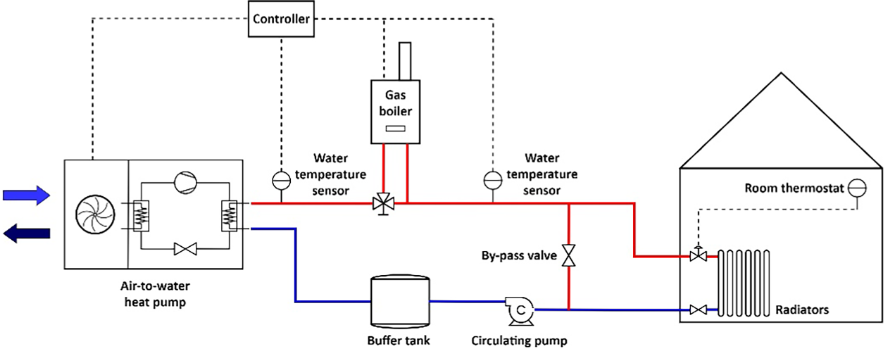
\includegraphics[width=0.6\linewidth]{hhsawhpboiler}
    \caption{\acs{HHS} with an \acs{AWHP} and condensing gas boiler \cite{dongellini_influence_2021}}
    \label{fig:hhsawhpboilerdiagram}
\end{figure}

TODO: Explicitly define what a hybrid heating system is à la Klein and Huchtemann mentioning bivalency, set-point temp, T_biv, show plot, etc. 



\subsection{Buffer Tank} 
A buffer tank is a medium- to large-sized water vessel used in hydronic heating systems. It provides a large thermal inertia to the heating system-house system, which many small- to medium-sized houses, especially those with poor insulation, lack. Thermal inertia is a desired property of a building as rapid thermal fluctuations in ambient air are less of a concern when it comes to maintaining a comfortable thermal environment indoors. This effect is noticeable in large office/district buildings with high thermal inertias and plays a significant role in heating-capacity selection \cite{owen_ashrae_2009}. Furthermore, a buffer tank provides a ``hydraulic switch'' and allows for heat generation and heat distribution to be in separate loops. This opens up the option to have differing flowrates between the heat generation and heat distribution loops. 

Buffer tanks have been found, when sized correctly and with an appropriate control strategy, to have a positive influence on the efficiency and performance on \acp{HHS} \cite{klein_numerical_2014,roccatello_analysis_2022}. The controller is able to make use of the \HPs ``most profitable working conditions'' thanks to the presence of the buffer \cite{dettorre_economic_2018}. It has been found that when a buffer thank is present in the \HP circuit, \ac{SPF} increases as the size of the \HP decreases \cite{mugnini_variable-load_2021}. \citeauthor{mugnini_variable-load_2021} confirmed this for all sizes of \HPs simulated, the smallest buffer tank having a capacity of \SI{200}{\liter}. 

The larger a buffer tank in volume, the larger its energy storage capacity. However, with a larger volume, and naturally larger cylinder and surface area, comes greater heat loss, which seem to correlate almost linearly \cite{klein_numerical_2014}. This could be justified if other performance factors such as \ac{SPF} or load factor were positively affected to offset this loss in heat, however this does not seem to be the case according to \cite{roccatello_analysis_2022} and \citeauthor{klein_numerical_2014}, which also found only a moderate reduction in on-off cycles with smaller tanks. This is partly to do with the thermal inertia of the building and return temperature controller. 
\citeauthor{klein_numerical_2014} found that the volume of the buffer tank had very limited effect on the system performance. \citeauthor{dongellini_influence_2021} sized their buffer tank just large enough such that the maximum number of on-off cycles was never greater than six per hour,  resulting in a buffer tank with a volume of \SI{79}{\litre}.  This maximum on-off cycle figure was chosen based off their \HP manufacturer guidelines. Daiken suggest %FIND SUGGESTED MAX NUMBER OF ON-OFF CYCLES FROM DAIKIN. 
\cite{dettorre_economic_2018}

\subsection{Frosting and Defrosting}
Frosting occurs in \acp{ASHP} in colder ambient temperatures resulting in issues for \HPs. Frost build up depends on the ambient temperature, temperature of the surface in question and relative humidity. For heat pumps, a few ranges of temperatures at which frosting occurs has been found in the literature \cite{sandstrom_frosting_2021} finding a range of \qtyrange{-15}{6}{\celsius} at a r.h. of $\approx$90, while \cite{kropas_experimental_2021} found frost formation to begin when the ambient air temperature was below \SI{3.5}{\celsius} with a r.h. of 88\%. Frosting specifically occurs when the surface temperature of the fins on the air-side heat exchanger component (evaporator) are lower than the dew point of the of the air. Water droplets start to form and collect on the fins. When the temperatures is below freezing or close to it, the water droplets freeze to the fins and build up a frosting. Frost, unlike snow, which both form from the freezing of water droplets, is not loose and must be scraped off or melted off. It will not \textit{fall off of} a surface like snow might. This layer of frost acts as a layer of insulation and restricts the heat exchanger from transferring heat from the ambient air. Since these fins are typically closely packed, if the layering of frost continues and progressively builds up, the airflow around the fins decreases and so does convective heat transfer to the ambient air, further exacerbating the issue of insulation. All of this is to say that when frosting occurs in \acp{ASHP}, their performance declines severely. \cite{zhang_experimental_2018} found that the temperature of the air and surface of the fins, humidity, velocity of air are the main factors involved in frost formation. 

Many treatments for frosting have been proposed and implemented into products. There is however no golden bullet solution, all of their advantages and disadvantages. Three main solutions are typically used when addressing the issue of frosting in \acp{ASHP}. 
\begin{itemize}
    \item Simple on-off defrosting: the \HP is simply switched off when too much frost has formed on the outdoor component. The performance has been degraded to such a point that it is now economically advantageous to turn off the \HP and wait for the frost to melt away. This however, takes a long time and can negatively affect the thermal comfort of a home if no other heat production is used. The \HP does not use any power during this off-cycle of course, retaining the \ac{COP} of the \HP --- although, this may affect the overall system performance if a gas boiler needs to be used to provide the entire heating load of the home.
    \item Reverse cycle defrosting: this method is similar to the first method; the refrigerant is cycled in reverse and hot gas is forced into the heat exchanger. Recall that \HPs and refrigerators differ only in objective. The \HP now treats the outdoors as the ``cold'' sink and begins transferring heat from indoors to outdoors. Intuitively, one can see that this is quite detrimental to the performance of the \HP as the house is being actively cooled in order to heat up the outdoor coils and fins to melt away the frost, and one cannot forget water's high thermal capacity... The intention in this method is to melt the frost much quicker than the first method, allowing the \ASHP to being warming the home once again much earlier than the the simple on-off defrosting method.
    \item Resistive heating: electric resistive heaters are installed on/in the heat exchanger. This method works very well, quickly melting off frost and is a separate heating element to the \HP and therefore does not interrupt the \HPs cycles. Resistive heaters are very expensive to run and negatively affect the \ac{COP} of the \HP.
\end{itemize}

\cite{amer_review_2017} found that the reverse cycling method resulted in a higher \ac{COP} than the other two methods. 

\section{Heating Degree Days and Design Temperatures} \label{sec:hddanddesign}
\acp{HDD} is a measure of the difference between the outside temperature and the inside temperature. \acp{HDD} are usually considered over a period of time, be it a month, heating season or entire year. A \textit{base} temperature is chosen, typically around \qtyrange{12}{21}{\celsius} which then determines when it is ``cold'' outside, or can be thought of as being the temperature above which heating is no longer considered to require heating. This base temperature can be chosen at will, and simply depends on what the person/institution deems to be \textit{warm enough}. This measure can be used to quantitatively compare the heating demand of a given house in different locations/climates. The heating requirement of a specific building are directly proportional to the \ac{HDD} \cite{chartered_institution_of_building_services_engineers_environmental_2006}.

To calculate  the \ac{HDD} for a certain day, three equations are used and are displayed from \cref{eq:hdd}. Which equation to use is determined by the interaction between the base temperature and the maximum temperature recorded during that day.  

\begin{align}\label{eq:hdd}
    \text{Degree days} = \begin{cases}
        t_\text{base} - \frac12(t_\text{max} + t_\text{min}), & \text{if } t_\text{max} < t_\text{base}\\
        \frac12(t_\text{base} - t_\text{min}) -\frac14(t_\text{max} -t_\text{base} ), & \text{if } t_\text{base} > \frac12(t_\text{max} + t_\text{min}) \\
        \frac14(t_\text{base} -t_\text{min} ), & \text{if } t_\text{base} <\frac12(t_\text{max} + t_\text{min})
     \end{cases}  
\end{align}

To calculate the Monthly degree days however, only \cref{eq:hdd1} is made use of. This total is found by summing the daily temperatures differences and can be seen in \cref{eq:mdd}.
\begin{equation}
    \text{Monthly degree days} = \displaystyle\sum_\text{month} \left[t_\text{base} - \frac12(t_\text{max} + t_\text{min})\right] \label{eq:mdd}
\end{equation}

\citetitle{chartered_institution_of_building_services_engineers_environmental_2006} has chosen a base temperature of \SI{15.5}{\celsius}. \citetitle{owen_ashrae_2009} used a base temperature of \SI{18.3}{\celsius} and determined an annual \ac{HDD} of \SI{3135}{\celsius\day} for Dublin Airport, IE, N\ang{53;26;} W\ang{06;15;}. Using the online tool \texttt{Degree Days.Net} \cite{degreedays} with a base temperature of \SI{15.5}{\celsius}, a \ac{HDD} figure of \SI{2072.3}{\celsius\day} was obtained for the same location.  

Design temperatures are a measure how many hours/days a specified condition is exceeded. In the case of a heating design temperature, this would indicate how many days of the year or heating season are spent below a given temperature. \citetitle{owen_ashrae_2009} notes that this measure does not give an indication of the frequency or duration of these events, only a cumulative result is returned. According to \citetitle{owen_ashrae_2009}, the 99.6\% design temperature in Dublin Airport is \SI{-1.9}{\celsius} while the 99.0\% design temperature is \SI{-0.7}{\celsius}. Traditionally, conventional gas boilers or resistive heaters were sized to design temperatures, meaning, for a chosen design temperature percentile (e.g., 99.0\%), the heater could heat the building to thermally comfortable levels for 99\% of the year, however during the 1\% temperature lows, the heater would not be adequate. This calculates to the heater being undersized for $\sim$35 hours of the year. \graffito{$365\times24=\SI{8860}{\hour} \Rightarrow 99.0\%\text{-ile} = 8760(100-99.0) = 87.6$ }

In monovalent systems, the \HP is sized in such a way as to be able to provided the entire heating load for a building at design conditions. This results in the \HP being positively over-dimensioned for the task \cite{klein_numerical_2014}. 

The concept of a \textit{design-day} can be used to design heating configurations for homes, especially when performing numerical simulations on a model of the system \cite{rauschkolb_cost-optimal_2020}. A design-day file is a special weather file created with design conditions in mind. Based on the design temperature parameter, \citelist{owen_ashrae_2009}{institution} lays out a procedure to generate a 24-hour weather profile. These profiles represent the 0.4\% to 99.6\% extremes experienced for a particular location. This weather data is used in simulations to determine the minimum size for a heater required for a house (for these particular percentiles of course). \graffito{for the purposes of the simulation(s) concerning this thesis, the 0.4 percentile, and any cooling-nessecary-temperatures for that matter, are not of concern as cooling is out of scope.}

The ``heating duration curve'' can be devised for a specific climate and a specific \HP where a curve is plotted on a chart with heating load [\unit{\kilo\watt\per\hour}] against number of hours the heating load is equal to or above a selected percentage of design load. For example, as illustrated in \cref{fig:heatingloaddurationcurve}, the blue line indicates 50\% design load, and lands around 1300 hours on the $x$-axis. This means that for 1300 hours of the year/heating season, the heating load of the building is 50\% of the design (or max) load. The balance point marked by the yellow circle is the point at which the \HP is not longer able to provide the entire heating load required by the building. To the left of this point, the gas boiler will need to provide the remaining heat capacity to maintain a comfortable indoor temperature. If the \ac{AWHP} size is increased, this balance point moves to the left, as the \HP can provide the entire heating envelope of the building at lower temperatures. Of course, for the sake of the diagram, the curves and lines in this figure are arbitrary (e.g., \ac{AWHP} performance is not linear with outdoor temperature, and by proxy, heating load), but it illustrates how a \HP may be sized to 60\% of the design load of a building.

\begin{figure}[htb]
    \centering
    \import{tikz/}{heatingDurationCurve.tex}
    \caption{Heating Duration Curve}
    \label{fig:heatingloaddurationcurve}
\end{figure}

All of this is to say that there are many methods of determining and comparing the heating load of a building for a given climate, with which heating devices may be sized to in order to be able to (almost always) have the capacity to heat a building. A \ac{HHS} is unique in that it is composed of two heating devices. The boiler, as stated before, is sized to a certain high-percentage design condition. This may be defined by the user/homeowner, convention, or by some set of standards set by a governing body (e.g., ASHRAE), and is typically a value in the region of 95\% to 99.7\%. On account of this, the \ac{AWHP} can be sized smaller than compared to if it were the sole heating device.

\section{Primary Energy}\label{sec:primaryenergy}
\ac{PE} is a term used in the fields of energy statistics and energetics. Sources of \ac{PE} are those which have not been interfered with by humans, in other words, are the natural form of energy and are unprocessed. \ac{PE} sources include: oil, natural gas, sunlight, wind, etc. \ac{PE} stands in contrast to secondary energy, which can be thought of as the carrier of energy, which most commonly happens to be electricity, but can also be liquid forms of energy (e.g., diesel/petrol, ), hydrogen fuel cells or (waste) heat. Following from \ac{PE}, is \ac{PEF} which connects \ac{PE} to final energy, it is a measure of how much energy in total is required to produce a unit of \textit{usable} energy. \cref{fig:PEtoFinalSankey} is a sankey diagram which breaks down the flow of energy in Ireland in 2020 from \ac{PE} on the left by fuel type, and final energy on the left, by sector. It also highlights the energy losses associated with energy production and transmission. It requires energy to convert natural gas or oil to electricity, while energy losses corresponding to renewable energy production are dismissed, as the energy source is of course \textit{free}. 

\begin{figure}[htb]
    \centering
    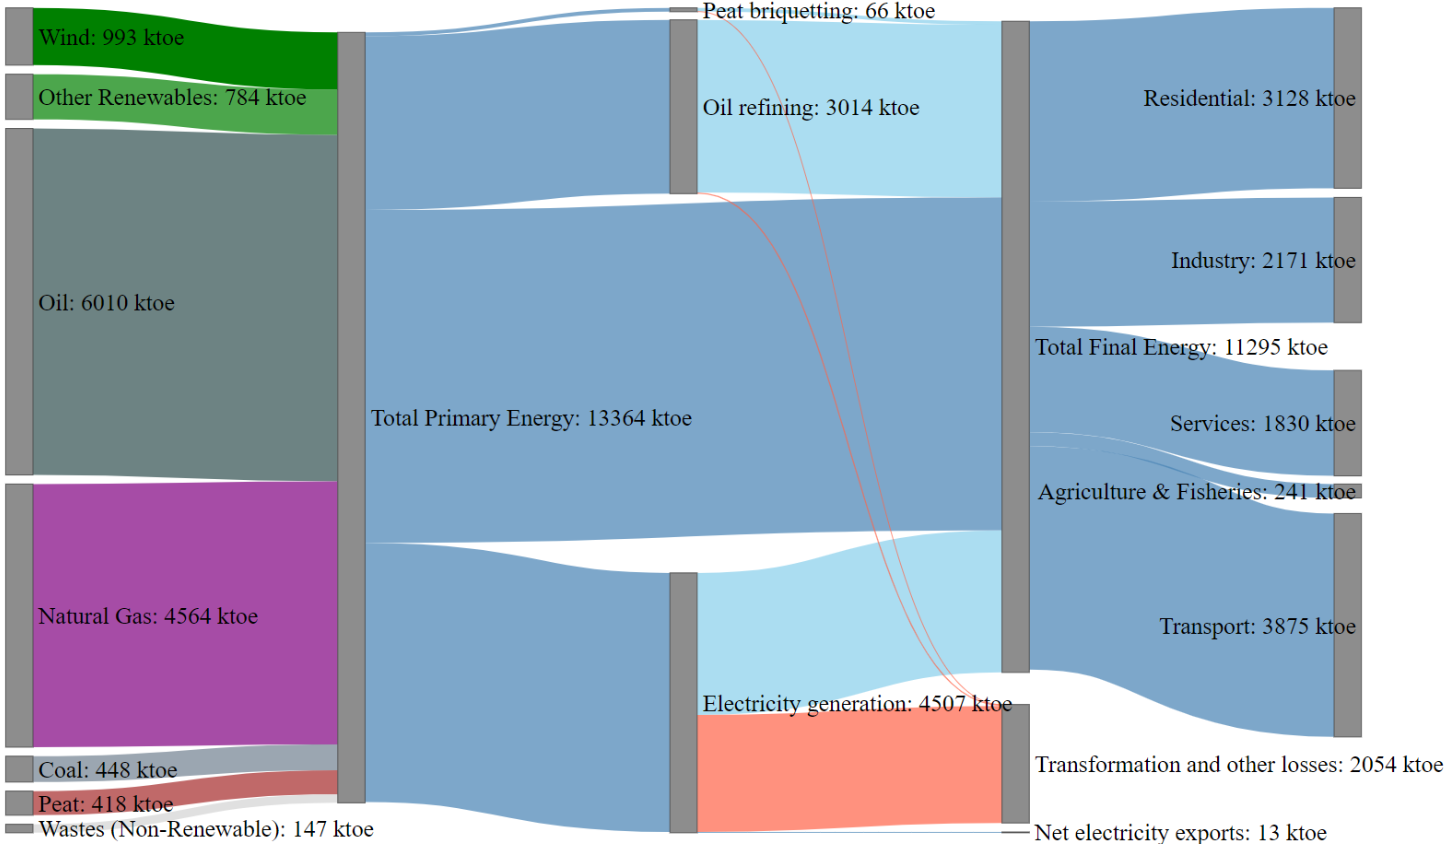
\includegraphics[width=0.7\linewidth]{primaryEnergyToFinalEnergySankey}
    \caption[\acs{PE} breakdown by fuel type and sector]{Sankey diagram showing \acs{PE} by fuel type on left and final energy by sector on right \cite{seai_energy_2021}.}
    \label{fig:PEtoFinalSankey}
\end{figure}

\ac{PES} is difference between the amount of energy consumed by the original device (whatever it may be) and the amount of energy consumed by the new device. In relation to this thesis, it will be taken to be the savings of the new heat generation system compared to the old system (conventional gas boiler). Knowledge of the \ac{PEF} (or \ac{RES}) and \ac{PES} can indicate how much $\text{CO}_2$ with a new heating system, and is the foundation of the techno-ecological model of this thesis. 

\section{Electrification of Heating}
The EU has now for a number of years been pushing for the electrification of heating throughout the union. This has been identified as a clear means to achieve decarbonisation goals, as concerns over global warming become greater. As noted in \cref{sec:context}, the residential sector contributes 27\% of the final energy consumption, while residential domestic water production and space heating contributes to 80\% of that. In Ireland, residential heating accounted for 53\% of $\text{CO}_2$ emissions from heating. However, across all sectors, heating and cooling are responsible for half of all final energy consumption in the EU \cite{an2016strategy}. Therefore, it is clearly evident that decarbonisation of the heating/cooling sector is vital to a) reaching EU targets of lowering $\text{CO}_2$ emissions and b) improving air quality and the reduction of harmful emissions \cite{epri2018us}. Although, switching to electrically driven heating systems does not automatically or inherently reduce the carbon emissions, merely, it changes the source of the energy; the electricity must also be decarbonised for this to be the case. 

\citeauthor{seai_energy_2021} \cite{seai_energy_2021} carried out a comprehensive study on the Irish electrical grid performance as it relates to renewable energy sources and to heating/cooling. According to the report: the share renewable energy to that of the the total energy used in 2020 was 13.5\% (having missed the EU target of 16\%); the share of renewable energy used specifically in heating/cooling was just 6.3\%, its target having been 12\%; energy from renewable sources grew by 8.9\% over the previous year, and the total installed wind energy capacity grew by 4.1\%, from \SI{4130}{\mega\watt} to \SI{4310}{\mega\watt} (in the Republic). Overall, the residential energy $\text{CO}_2$ emission has trending downwards over the past decade and a half, falling by 25\% since 2005, and the $\text{CO}_2$ intensity of electricity generation is half of its value in 2005, standing at \SI{300}{\gram CO\textsubscript{2}\per\kilo\watt\hour}. \graffito{Emission intensity is a measure of how much $\text{CO}_2$ is released per unit of energy produced}. These are good signs for the electrification of heating, because in order for the electrification of heating to result in a decarbonising of heating, the electricity production must at least have a lower emission intensity compared to if no electrification process were to take place, but ideally have the prospects of becoming a very low/zero $\text{CO}_2$ intensity matter.

\section{Controllers and Control Theory}
Control theory is concerned with the control of dynamic systems with with a desired goal in mind, which is called the reference. A controller manipulates the inputs to a system, usually denoted $u$ in such a way as to alter the output variables or states, $y$, of the system to follow a given reference. Disturbances $d$ to a system are expected, yet unforeseen inputs to a system which may significantly alter the outputs state.  There are two main types of controller, feed-forward, and feedback controllers.

A feed-forward controller, also known as an open loop controller, controls the system without knowing the current state of the system. This is possible if disturbances are either eliminated, or wholly understood and accounted for.\graffito{However, they would they no longer qualify as disturbances, and would simply be considered as inputs, but that is by the by.} Complete knowledge of the dynamics of the system being controlled would be required and captured by a mathematical model, either by physics and first principles, or by system identification (a model is fitted to data). The dynamics of the system are inverted by the controller and fed to the system as inputs. Any error in the inversion process results in undesired system states. 

Feedback controllers, also known as closed loop controllers are a \textit{much} more common form of controller. The current system state is known to the controller, and the reference and current state information is used to determine the appropriate control inputs. In doing so, a feedback controller inherently changes the dynamics of a system. Feedback controllers usually make systems more stable, however, there is the possibility of making systems less stable and even unstable through controllers. There are many types of feedback controllers, the most common and well understood kind being a linear feedback controller called a \ac{PID} controller, or just a \ac{PID}. Linear controllers assume the general behaviours of the system to be linear. Although, even if the dynamics of system are not, in fact, linear, a \ac{PID} will still likely be able to control the system appropriately and reach the reference state.

In a hybrid heating system, controllers are used to manage the operation of the different heating technologies and ensure that they are used in the most efficient and effective way possible. The controllers in a hybrid heating system are typically responsible for a number of tasks, including monitoring the temperature inside and outside the building, determining the best heating technology to use based on the current conditions, and controlling the operation of the heating technologies to maintain a comfortable and consistent temperature.

For example, when the outside temperature is cold, the controller may determine that it is most efficient to use the gas furnace to heat the building. When the outside temperature is mild, the controller may determine that it is more efficient to use the heat pump, which uses less energy than the gas furnace. Very advanced controllers may also use predictive algorithms and weather forecasts to anticipate changes in temperature and adjust the heating system accordingly by storing a lot of heat in the buffer tank during a warm period right before a cold period \cite{demirezen_feasibility_2021}.

\subsection{\acs{PID} Controllers}
\ac{PID} controllers are a type of feedback control system that are commonly used in a wide variety of systems to maintain a desired output or setpoint. The acronym refers to the three components of the control algorithm used by the controller. \ac{PID} controllers work by continuously calculating an error value that represents the difference between the desired setpoint and the current output of the system. This error value is then used to calculate and apply a correction to the system, based on the three components of the \ac{PID} algorithm:
\begin{itemize}
    \item The proportional component applies a correction proportional to the error value. This allows the controller to quickly respond to large errors and make large corrections.
    \item The integral component applies a correction based on the accumulated error over time. This helps to eliminate steady-state errors and ensure that the system eventually reaches the desired setpoint.
    \item The derivative component applies a correction based on the rate of change of the error. This helps to dampen the system's response and prevent overshoot and oscillation.  
\end{itemize}


\ac{PID} controllers are used in a wide variety of systems, including mechanical systems like motors and actuators, temperature control systems, and chemical process control systems. They are often preferred over other control algorithms because they are relatively simple to implement and can provide stable and accurate control of the system's output.

\subsection{Noise and Error}
Noise and error are common sources of problems in control systems. Noise refers to random variations in the system's output that are not caused by the control signal, while error refers to the difference between the desired setpoint and the actual output of the system. Noise and error can have a number of adverse effects on the performance of a control system, including reduced accuracy and stability, as well as increased oscillation and overshoot. To deal with noise and error in control systems, a number of different approaches can be used. One approach is to use a filter to remove noise from the system's output signal. This can be done using a low-pass filter, which removes high-frequency noise, or a high-pass filter, which removes low-frequency noise. Another approach is to use a model-based control algorithm, which uses a mathematical model of the system to predict the system's output and apply appropriate control signals. This can help to reduce the effects of noise and error by using the model to compensate for them. Furthermore, another approach is to use a robust control algorithm, which is designed to be resistant to the effects of noise and error. Robust control algorithms typically use a combination of feedback and feed-forward control, as well as advanced control techniques like gain scheduling and optimization, to achieve robust performance in the presence of noise and error.




% \ctparttext{You can put some informational part preamble text here.
% Illo principalmente su nos. Non message \emph{occidental} angloromanic
% da. Debitas effortio simplificate sia se, auxiliar summarios da que,
% se avantiate publicationes via. Pan in terra summarios, capital
% interlingua se que. Al via multo esser specimen, campo responder que
% da. Le usate medical addresses pro, europa origine sanctificate nos se.}
%\part{Model and Results}\label{pt:showcase}
%************************************************
\chapter{The Model}\label{ch:model} 
%************************************************
Write about the model and how it was built.
3D model of house was provided...
Used software \texttt{Modelica}...

%************************************************
\chapter{System Model}\label{ch:model} 
%************************************************
%VWrite about the model and how it was built. 3D model of house was provided... Used software \texttt{Modelica}...
%Demonstate how model (acturately) predicts how the residential home behaves in real life to certain degree... Compare simulation to real life restults... Explain inaccuracies... which assumptions lead to these...
% Thermodynamic model, assumptions, constraints, design point conditions etc. 
% Equations 
% economic and ecological models. 

% \begin{flushright}{\slshape
%     The purpose of models is not to fit the data, but to sharpen the question} \\ \medskip
%     --- Samuel Karlin
% \end{flushright}

\section{Timestep and solver}
A nominal timestep of 3 minutes was chosen, as this results in a very accurate simulation run. The dynamics of the model are accurately captured by a timestep of 180 seconds. The timestep value used in the simulations in the literature is sparse, however, \citeauthor{roccatello_analysis_2022} \cite{roccatello_analysis_2022} use five-minute timesteps, while \citeauthor{dongellini_influence_2021} \cite{dongellini_influence_2021} use timesteps of 30 seconds, \citeauthor{klein_numerical_2014} \cite{klein_numerical_2014} also use timesteps of 3 minutes. The \texttt{Dymola} built-in \texttt{Radau II-A} solver was used, as this is recommended by the Buildings Library Best Practices \cite{lawrence_berkeley_national_laboratory_user_2022}, which also suggests a tolerance of \num{1E-6} for ``faster and more robust simulation for thermo-fluid flow systems''. 

The \texttt{Radau II-A} solver uses the user-inputted timestep as a nominal value, but can dynamically decrease the timestep in order to maintain stability or accuracy. Thus, even though there are \num{175200} three-minute intervals in a year, during each simulation run there tends to be circa \num{180000} timesteps. 

\section{Location} \label{sec:location}
The reference house that the building model is based off of a hipped dormer, two-storey residential house located in Belturbet, Cavan, a small town close to the Republic of Ireland and Northern Ireland border, about 125 kilometres from Dublin. The reference house lies at an elevation of 80 metres and is Easterly facing. The dwelling is located in a residential estate, and is thus classified as being located in an urban environment.

\section{Form and Fabric}
The reference model has a floor area of 160 square metres, 93 square metres of which are downstairs, i.e., ``exterior floor'', a gross roof area of 173 square metres and a total external wall surface area of 139 square metres. There are 21 exterior windows of varying sizes in total and thirteen rooms, seven downstairs and six upstairs. The ceiling height is a uniform 2.5 metres throughout the model. All rooms except for one were considered to be unconditioned, the exception being a very small box room on the ground floor which was interpreted to be a utility room of sorts. The void zones were also unconditioned. The building model geometry and thermal properties were created during previous works by \citeauthor{keogh_technical_2018} \cite{keogh_technical_2018}. A floor plan schematic can be seen in \cref{fig:floorplan}, showing the ground floor and first floor room layouts and windows. A 3D rendered model of the house can be seen in \cref{fig:3dmodel}. All building model data is contained in a \texttt{.idf}-file, an input data file interpretable by \texttt{EnergyPlus}. This file contains data about the geometry of the building, envelope construction, thermal and physical properties of the constructions, building and occupancy schedules, internal gains, outside air infiltration to void zones and various other data regarding the simulation process e.g., timestep. 

\begin{figure}[htb]
    \centering
    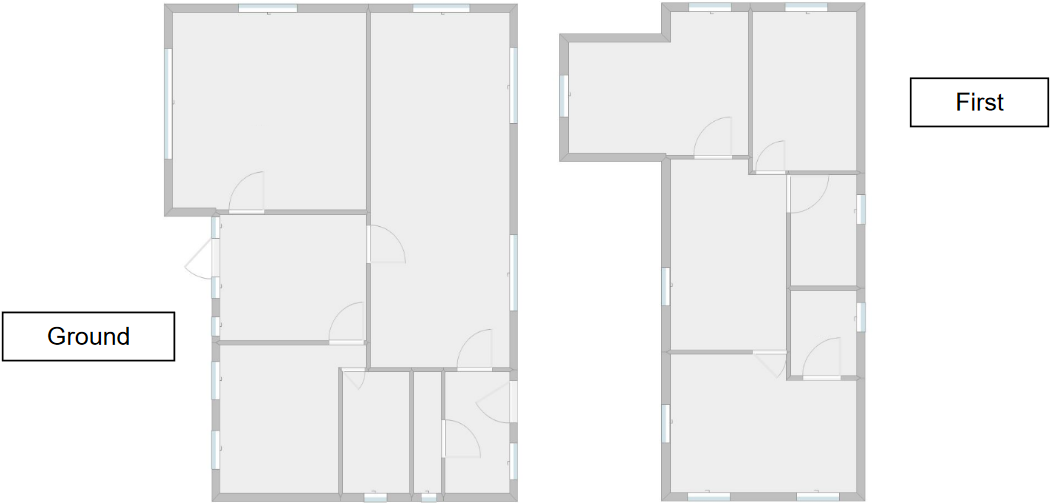
\includegraphics[width=0.75\linewidth]{dwellingFloorPlan}
    \caption{Dwelling floor plan, ground and first floor}
    \label{fig:floorplan}
\end{figure}

\begin{figure}[htb]
    \centering
    %\includegraphics[width=0.7\linewidth]{3dmodel}
    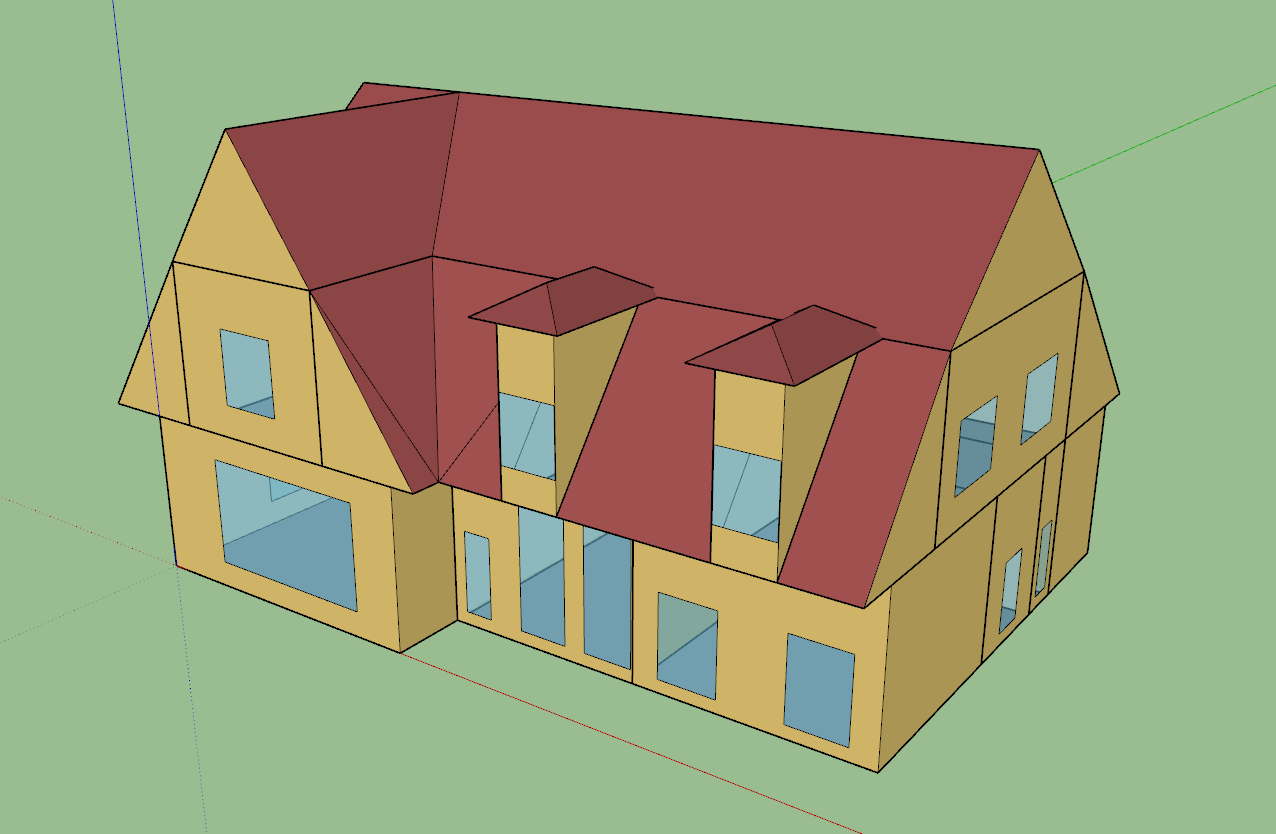
\includegraphics[width=0.7\linewidth]{Housepng.png}
    \caption[3D Model of Reference Building]{3D Model of Reference Building, rendered in \texttt{SketchUp} via the \texttt{Euclid} plugin}
    \label{fig:3dmodel}
\end{figure}


\subsection{Thermal Properties of Constructions}

\begin{table}[htb]
    \footnotesize
    \centering
    \caption{Summary of $U$-Values}
    \label{tbl:uvalues}  
    \begin{tabular}{lccccc}\toprule
        \multicolumn{1}{c}{\multirow{2}{*}{\begin{tabular}[c]{@{}c@{}}Building \\ Model\end{tabular}}} & \multicolumn{4}{c}{\begin{tabular}[c]{@{}c@{}}$U$-Value\\ {[}\unit{\watt\per\square\meter\per\kelvin}{]}\end{tabular}} & \multirow{2}{*}{\begin{tabular}[c]{@{}c@{}}Infiltration\\ Rate\\ {[}\acs{ACPH}{]}\end{tabular}} \\ \cmidrule(lr){2-5}
        \multicolumn{1}{c}{} & \begin{tabular}[c]{@{}c@{}}Exterior\\ Wall\end{tabular} & \begin{tabular}[c]{@{}c@{}}Pitched\\ Roof\end{tabular} & \begin{tabular}[c]{@{}c@{}}Exterior\\ Floor\end{tabular} & \begin{tabular}[c]{@{}c@{}}Exterior\\ Glazing\end{tabular} &  \\ \midrule
        \begin{tabular}[c]{@{}l@{}}Minimal\\ Retrofit\end{tabular} & \num{0.31} & \num{0.16} & \num{0.25} & \num{2.15} & \num{0.8} %\\
        %\begin{tabular}[c]{@{}l@{}}Deep 
            %\\ Retrofit\end{tabular} & \num{0.18} & \num{0.16} & \num{0.18} & \num{1.39} & \num{0.5} 
            \\ \bottomrule   
    \end{tabular}
\end{table}

\subsubsection{Minimal Retrofit Model}
\cref{tbl:extwallconst} details the specifications of the exterior wall construction for the minimal retrofit model, from outside to inside. 
\begin{table}[htb]
    \footnotesize
    \centering
    \caption{Exterior Wall Construction}
    \label{tbl:extwallconst}
    \begin{tabular}{lcccc}
        \toprule
        Layer        & \multicolumn{1}{c}{\begin{tabular}[c]{@{}c@{}}Thickness \\ {[}m{]}\end{tabular}} & \multicolumn{1}{c}{\begin{tabular}[c]{@{}c@{}}Density \\ {[}\unit{\kilogram\per\cubic\meter}{]}\end{tabular}} & \multicolumn{1}{c}{\begin{tabular}[c]{@{}c@{}}Heat Capacity \\  {[}\unit{\joule\per\kilogram\per\kelvin}{]}\end{tabular}}  & \multicolumn{1}{c}{\begin{tabular}[c]{@{}c@{}}Conductivity \\   {[}\unit{\watt\per\meter\per\kelvin}{]}\end{tabular}} \\ \midrule
        Rainscreen   & \num{0.01}              & \num{7824}                & \num{500}                        & \num{30}                       \\
        Insulation   & \num{0.085}             & \num{43}                  & \num{1210}                       & \num{0.03}                     \\
        Air Cavity      & \num{0.15}              & $-$                  & $-$                      &  $-$                  \\
        Gypsum board & \num{0.019}             & \num{800}                 & \num{1090}                       & \num{0.16}                     \\
        \bottomrule
    \end{tabular}
\end{table}

\cref{tbl:extfloorconst} details the specifications of the exterior floor construction for the minimal retrofit model, from top to bottom. The exterior floor is the floor which lays on top of the foundations and therefore conducts heat from the inside of the house to the ground. It consists of concrete at the bottom, insulation board, an air cavity and floor tiles on top.

\begin{table}[htb]
    \footnotesize
    \centering
    \caption{Exterior Floor Construction}
    \label{tbl:extfloorconst}
    \begin{tabular}{lcccc}
        \toprule
        Layer        & \multicolumn{1}{c}{\begin{tabular}[c]{@{}c@{}}Thickness \\ {[}m{]}\end{tabular}} & \multicolumn{1}{c}{\begin{tabular}[c]{@{}c@{}}Density \\ {[}\unit{\kilogram\per\cubic\meter}{]}\end{tabular}} & \multicolumn{1}{c}{\begin{tabular}[c]{@{}c@{}}Heat Capacity \\  {[}\unit{\joule\per\kilogram\per\kelvin}{]}\end{tabular}}  & \multicolumn{1}{c}{\begin{tabular}[c]{@{}c@{}}Conductivity \\   {[}\unit{\watt\per\meter\per\kelvin}{]}\end{tabular}} \\ \midrule
        Acoustic Tile   & \num{0.0191}            & \num{368}                 & \num{590}                        & \num{0.06}                     \\
        Air Cavity      & \num{0.15}              & $-$                  & $-$                      &  $-$                  \\
        Insulation      & \num{0.085}             & \num{43}                  & \num{1210}                       & \num{0.03}                     \\
        Concrete        & \num{0.1016}             & \num{1280}                 & \num{840}                       & \num{0.53}                     \\
        \bottomrule
    \end{tabular}
\end{table}


\cref{tbl:pitchroofconst} details the specifications of the pitched roof construction for the minimal retrofit model, from outside to inside. This construction is applied to the bulk of the roof and consists of clay tile, an air cavity, insulation board and then plasterboard.

\begin{table}[htb]
    \footnotesize
    \centering
    \caption{Pitched Roof Construction}
    \label{tbl:pitchroofconst}
    \begin{tabular}{lcccc}
        \toprule
        Layer        & \multicolumn{1}{c}{\begin{tabular}[c]{@{}c@{}}Thickness \\ {[}m{]}\end{tabular}} & \multicolumn{1}{c}{\begin{tabular}[c]{@{}c@{}}Density \\ {[}\unit{\kilogram\per\cubic\meter}{]}\end{tabular}} & \multicolumn{1}{c}{\begin{tabular}[c]{@{}c@{}}Heat Capacity \\  {[}\unit{\joule\per\kilogram\per\kelvin}{]}\end{tabular}}  & \multicolumn{1}{c}{\begin{tabular}[c]{@{}c@{}}Conductivity \\   {[}\unit{\watt\per\meter\per\kelvin}{]}\end{tabular}} \\ \midrule
        Clay Tile   & \num{0.025}            & \num{1900}                 & \num{800}                        & \num{0.84}                     \\
        Air Cavity      & \num{0.15}              & $-$                  & $-$                      &  $-$                  \\
        Insulation      & \num{0.162}            & \num{43}                  & \num{1210}                       & \num{0.03}                     \\
        Gypsum board & \num{0.019}             & \num{800}                 & \num{1090}                       & \num{0.16}                     \\
        \bottomrule
    \end{tabular}
\end{table}

The dormer roof provides no insulation and is only in place to protect the inside spaces from wind and rain. Its specifications can be read in \cref{tbl:dormerroofconst}.
\begin{table}[htb]
    \footnotesize
    \centering
    \caption{Hipped Dormer Roof Construction}
    \label{tbl:dormerroofconst}
    \begin{tabular}{lcccc}
        \toprule
        Layer        & \multicolumn{1}{c}{\begin{tabular}[c]{@{}c@{}}Thickness \\ {[}m{]}\end{tabular}} & \multicolumn{1}{c}{\begin{tabular}[c]{@{}c@{}}Density \\ {[}\unit{\kilogram\per\cubic\meter}{]}\end{tabular}} & \multicolumn{1}{c}{\begin{tabular}[c]{@{}c@{}}Heat Capacity \\  {[}\unit{\joule\per\kilogram\per\kelvin}{]}\end{tabular}}  & \multicolumn{1}{c}{\begin{tabular}[c]{@{}c@{}}Conductivity \\   {[}\unit{\watt\per\meter\per\kelvin}{]}\end{tabular}} \\ \midrule
        Clay Tile   & \num{0.025}            & \num{1900}                 & \num{800}                        & \num{0.84}                     \\
        Air Cavity      & \num{0.15}              & $-$                  & $-$                      &  $-$                  \\
        Roofing Felt      & \num{0.005}            & \num{960}                  & \num{837}                      & \num{0.19}                    \\
        \bottomrule
    \end{tabular}
\end{table}

\begin{table}[htb]
    \footnotesize
    \centering
    \caption{External Glazing Construction}
    \label{tbl:glazingconst}
    \begin{tabular}{lccc}
        \toprule
        Layer        & \multicolumn{1}{c}{\begin{tabular}[c]{@{}c@{}}Thickness \\ {[}m{]}\end{tabular}} & \multicolumn{1}{c}{\begin{tabular}[c]{@{}c@{}}Transmittance \\ {[}\unit{\kilogram\per\cubic\meter}{]}\end{tabular}}  & \multicolumn{1}{c}{\begin{tabular}[c]{@{}c@{}}Conductivity \\   {[}\unit{\watt\per\meter\per\kelvin}{]}\end{tabular}} \\ \midrule
        Inner Pane   & \num{0.003}            & \num{0.783}                 & \num{0.4}                                         \\
        Argon Gas      & \num{0.20}              & $-$                  & $-$                                   \\
        Outer Pane     & \num{0.003}            & \num{0.783}                  & \num{0.4}                                    \\
        \bottomrule
    \end{tabular}
\end{table}

% \subsubsection{Deep Retrofit Model}
% During the deep retrofit process, the external wall, exposed floor and external glazing constructions are upgraded to conform to the Building Regulations Part L 2022. The infiltration rate was also decreased to 0.5 \ac{ACPH} due to leakiness being heavily reduced.

% \begin{table}[htb]
%     \footnotesize
%     \centering
%     \caption{External Glazing Construction (Deep Retrofit)}
%     \label{tbl:deepglazingconst}
%     \begin{tabular}{lccc}
%         \toprule
%         Layer        & \multicolumn{1}{c}{\begin{tabular}[c]{@{}c@{}}Thickness \\ {[}m{]}\end{tabular}} & \multicolumn{1}{c}{\begin{tabular}[c]{@{}c@{}}Transmittance \\ {[}\unit{\kilogram\per\cubic\meter}{]}\end{tabular}}  & \multicolumn{1}{c}{\begin{tabular}[c]{@{}c@{}}Conductivity \\   {[}\unit{\watt\per\meter\per\kelvin}{]}\end{tabular}} \\ \midrule
%         Inner Pane   & \num{0.003}            & \num{0.783}                 & \num{0.4}                                         \\
%         Argon Gas      & \num{0.20}              & $-$                  & $-$                                   \\
%         Middle Pane   & \num{0.003}            & \num{0.783}                 & \num{0.4}                                         \\
%         Argon Gas      & \num{0.20}              & $-$                  & $-$                                   \\
%         Outer Pane     & \num{0.003}            & \num{0.783}                  & \num{0.4}                                    \\
%         \bottomrule
%     \end{tabular}   
% \end{table}

% \begin{table}[htb]
%     \footnotesize
%     \centering
%     \caption{Exterior Floor Construction}
%     \label{tbl:deepextfloorconst}
%     \begin{tabular}{lcccc}
%         \toprule
%         Layer        & \multicolumn{1}{c}{\begin{tabular}[c]{@{}c@{}}Thickness \\ {[}m{]}\end{tabular}} & \multicolumn{1}{c}{\begin{tabular}[c]{@{}c@{}}Density \\ {[}\unit{\kilogram\per\cubic\meter}{]}\end{tabular}} & \multicolumn{1}{c}{\begin{tabular}[c]{@{}c@{}}Heat Capacity \\  {[}\unit{\joule\per\kilogram\per\kelvin}{]}\end{tabular}}  & \multicolumn{1}{c}{\begin{tabular}[c]{@{}c@{}}Conductivity \\   {[}\unit{\watt\per\meter\per\kelvin}{]}\end{tabular}} \\ \midrule
%         Acoustic Tile   & \num{0.0191}            & \num{368}                 & \num{590}                        & \num{0.06}                     \\
%         Air Cavity      & \num{0.15}              & $-$                  & $-$                      &  $-$                  \\
%         Insulation      & \num{0.085}             & \num{43}                  & \num{1210}                       & \num{0.03}                     \\
%         Concrete        & \num{0.1016}             & \num{1280}                 & \num{840}                       & \num{0.53}                     \\
%         \bottomrule
%     \end{tabular}
% \end{table}

% \begin{table}[htb]
%     \footnotesize
%     \centering
%     \caption{Exterior Wall Construction}
%     \label{tbl:deepextwallconst}
%     \begin{tabular}{lcccc}
%         \toprule
%         Layer        & \multicolumn{1}{c}{\begin{tabular}[c]{@{}c@{}}Thickness \\ {[}m{]}\end{tabular}} & \multicolumn{1}{c}{\begin{tabular}[c]{@{}c@{}}Density \\ {[}\unit{\kilogram\per\cubic\meter}{]}\end{tabular}} & \multicolumn{1}{c}{\begin{tabular}[c]{@{}c@{}}Heat Capacity \\  {[}\unit{\joule\per\kilogram\per\kelvin}{]}\end{tabular}}  & \multicolumn{1}{c}{\begin{tabular}[c]{@{}c@{}}Conductivity \\   {[}\unit{\watt\per\meter\per\kelvin}{]}\end{tabular}} \\ \midrule
%         Rainscreen   & \num{0.01}              & \num{7824}                & \num{500}                        & \num{30}                       \\
%         Insulation   & \num{0.085}             & \num{43}                  & \num{1210}                       & \num{0.03}                     \\
%         Air Cavity      & \num{0.15}              & $-$                  & $-$                      &  $-$                  \\
%         Gypsum board & \num{0.019}             & \num{800}                 & \num{1090}                       & \num{0.16}                     \\
%         \bottomrule
%     \end{tabular}
% \end{table}



 

\section{Schedules, Equipment and Internal Gains}
Internal gains in the context of an energy building simulation of a residential home refers to the heat generated within the envelope by people, appliances, and lighting.

People generate heat through their activities and body heat, while appliances generate heat through their operation. Lighting generates heat due to the inefficiencies in converting electricity into light, and light ultimately being converted to heat energy.

In energy building simulation, internal gains are important to consider because they can significantly affect the energy balance of the building. If the internal gains are high, the building may require less heating, which can lead to energy savings. Conversely, if the internal gains are low, the building may require more heating, which can lead to increased energy consumption and costs \cite{buttitta_high-temporal_2020}. 

Internal gains are typically modelled as a heat input to the building, which is then factored into the overall energy balance of the building. The magnitude of internal gains is typically calculated based on the number of occupants, the types and number of appliances, and the lighting levels in the building.

\subsection{Occupancy Gains}
The magnitude of these gains depends on factors such as the number of occupants, their activity levels, and the duration of their stay in the building. It was decided that a house of the size of the reference home was sized for a total of four persons. 

In order to accurately model occupancy gains in a \ac{BEM}, it is important to use typical occupancy profiles in conjunction with typical metabolic rates for different tasks. A typical occupancy profile is a representation of the number of occupants in the building over time, while a typical metabolic rate is a measure of the heat generated by a person due to their physical activity. Different tasks require different amounts of energy, and therefore result in different levels of heat generation. For example, a person sitting quietly may have a lower metabolic rate than someone performing strenuous physical activity.

\citeauthor{buttitta_high-temporal_2020} \cite{buttitta_high-temporal_2020} developed a stochastic occupancy model which generates hourly occupancy schedules for up to five different types of occupancy profiles of residential buildings for an entire year, based off of data gathered from London, UK. For this thesis, an occupancy profile was chosen which represented the largest share of the population, and two schedules were drawn, one for the weekdays and one for the weekends. These schedules depict the number of persons occupying the dwelling at each hour of the day, and the weekday schedule is detailed in \cref{tbl:occupancysched}. The table shows the fraction of the (four) occupants in the home at the corresponding time interval. For the weekend schedule, it was assumed that all occupants remain home all day.

\begin{table}[htb]
    \centering
    \caption{Weekday Occupancy Schedules}
    \label{tbl:occupancysched}
    \begin{tabular}
        {lcr}
        \toprule
        Time & Fraction of Occupants \\
        \midrule
        \num[parse-numbers=false]{00}:\num[parse-numbers=false]{00} $\rightarrow$ \num[parse-numbers=false]{06}:\num[parse-numbers=false]{50} & \num{1.0}\\
        \num[parse-numbers=false]{06}:\num[parse-numbers=false]{50} $\rightarrow$ \num[parse-numbers=false]{07}:\num[parse-numbers=false]{30} & \num{0.75}\\
        \num[parse-numbers=false]{07}:\num[parse-numbers=false]{30} $\rightarrow$ \num[parse-numbers=false]{08}:\num[parse-numbers=false]{20} & \num{0.5}\\
        \num[parse-numbers=false]{08}:\num[parse-numbers=false]{20} $\rightarrow$ \num[parse-numbers=false]{18}:\num[parse-numbers=false]{20} & \num{0.0}\\
        \num[parse-numbers=false]{18}:\num[parse-numbers=false]{20} $\rightarrow$ \num[parse-numbers=false]{24}:\num[parse-numbers=false]{00} & \num{1.0}\\
        \bottomrule
    \end{tabular}
\end{table}

\citetitle{ashrae_ansiashrae_2010} \cite{ashrae_ansiashrae_2010} details the metabolic rate of people performing various tasks, given in Met units, as well as watts per square metre. An activity level schedule was quasi-arbitrarily assembled and is detailed in \cref{tbl:activitysched}. The table, which is very similar to the occupancy schedule in nature, shows the metabolic rate in watts per square metre for the corresponding time interval. \texttt{EnergyPlus} takes this metabolic rate and multiplies it by a value of \qty{1.8}{\square\meter}, deemed to be the standard surface area of a typical adult. As a reference, a rate of \qty{40}{\watt\per\square\meter} corresponds to sleeping, \qtyrange{50}{90}{\watt\per\square\meter} are non-strenuous activities such as lounging, reading, etc. and above \qty{100}{\watt\per\square\meter} corresponds to activities such as walking briskly and beyond.
 
\begin{table}[htb]
    \centering
    \caption{Activity Schedules}
    \label{tbl:activitysched}
    \begin{subtable}[t]{0.485\linewidth}
        %\centering
        \caption{Weekday Activity Schedule}
        \begin{tabular}
        {lr}
        \toprule
        Time & \multicolumn{1}{c}{\begin{tabular}[c]{@{}c@{}}Metabolic\\ rate\\ {[}\unit{\watt\per\square\meter}{]}\end{tabular}}   \\
        \midrule
        \num[parse-numbers=false]{00}:\num[parse-numbers=false]{00} $\rightarrow$ \num[parse-numbers=false]{06}:\num[parse-numbers=false]{50} & \num{40}\\
        \num[parse-numbers=false]{06}:\num[parse-numbers=false]{50} $\rightarrow$ \num[parse-numbers=false]{08}:\num[parse-numbers=false]{20} & \num{120}\\
        \num[parse-numbers=false]{08}:\num[parse-numbers=false]{20} $\rightarrow$ \num[parse-numbers=false]{18}:\num[parse-numbers=false]{20} & \num{0.0}\\
        \num[parse-numbers=false]{18}:\num[parse-numbers=false]{20} $\rightarrow$ \num[parse-numbers=false]{22}:\num[parse-numbers=false]{00} & \num{120}\\
        \num[parse-numbers=false]{20}:\num[parse-numbers=false]{00} $\rightarrow$ \num[parse-numbers=false]{23}:\num[parse-numbers=false]{10} & \num{75}\\
        \num[parse-numbers=false]{23}:\num[parse-numbers=false]{10} $\rightarrow$ \num[parse-numbers=false]{24}:\num[parse-numbers=false]{00} & \num{40}\\
        \bottomrule
    \end{tabular}
    \end{subtable}%
    \hfill
    \begin{subtable}[t]{0.485\linewidth}
        %\centering
        \caption{Weekend Activity Schedule}
        \begin{tabular}
        {lr}
        \toprule
        Time & \multicolumn{1}{c}{\begin{tabular}[c]{@{}c@{}}Metabolic\\ rate\\ {[}\unit{\watt\per\square\meter}{]}\end{tabular}} \\
        \midrule
        \num[parse-numbers=false]{00}:\num[parse-numbers=false]{00} $\rightarrow$ \num[parse-numbers=false]{01}:\num[parse-numbers=false]{00} & \num{75}\\
        \num[parse-numbers=false]{01}:\num[parse-numbers=false]{00} $\rightarrow$ \num[parse-numbers=false]{07}:\num[parse-numbers=false]{20} & \num{40}\\
        \num[parse-numbers=false]{07}:\num[parse-numbers=false]{20} $\rightarrow$ \num[parse-numbers=false]{09}:\num[parse-numbers=false]{30} & \num{75}\\
        \num[parse-numbers=false]{09}:\num[parse-numbers=false]{30} $\rightarrow$ \num[parse-numbers=false]{24}:\num[parse-numbers=false]{00} & \num{120}\\
        \num[parse-numbers=false]{20}:\num[parse-numbers=false]{00} $\rightarrow$ \num[parse-numbers=false]{23}:\num[parse-numbers=false]{10} & \num{75}\\
        \num[parse-numbers=false]{23}:\num[parse-numbers=false]{10} $\rightarrow$ \num[parse-numbers=false]{24}:\num[parse-numbers=false]{00} & \num{40}\\
        \bottomrule
        \end{tabular}
    \end{subtable}%
\end{table}

\subsection{Lighting}
In the past, internal gains from lighting used to be a significant contributor to the overall heat load of buildings. This was largely due to the widespread use of inefficient incandescent light bulbs, which generated a significant amount of heat as a byproduct of their operation. In fact, it was not uncommon for incandescent bulbs to emit more heat than light, resulting in a significant waste of energy and contributing to higher cooling loads in buildings.

However, with the gradual adoption of more efficient lighting technologies such as LED bulbs, internal gains from lighting have become much less of a concern. LED bulbs are significantly more efficient than incandescent bulbs, converting a higher percentage of their energy input into light rather than heat. This means that they generate far less waste heat, resulting in lower cooling loads and reduced energy consumption. \citefield{ISO17772}{shorttitle} presents lighting schedules and load density profiles for single family residential homes, and are reproduced in \cref{tbl:lightandequip}. 

\subsection{Plug Loads and Equipment}
Plug loads in a residential home refer to the energy consumed by appliances and devices that are plugged into electrical outlets, such as televisions, computers, and kitchen appliances. Equipment internal gains in a residential home refer to the heat generated by the operation of various equipment and appliances, such as refrigerators, ovens, and water heaters. This heat can contribute to the overall heat load of the home, particularly during periods of high use. \citefield{ISO17772}{shorttitle} gives details regarding standards for schedules and load density profiles for equipment gains and plug loads, and is reproduced in \cref{tbl:equipsch}, showing the fraction of the load thought to be ``active'' at the corresponding time. The nominal lighting load is given to be \qty{2.07}{\watt\per\square\meter} and nominal equipment load is given to be \qty{1.92}{\watt\per\square\meter}.

\begin{table}[htb]
    \centering
    \caption{Lighting, Plug Loads and Equipment Gains Schedules and Load Densities \cite{ISO17772}}
    \begin{subtable}[t]{0.485\linewidth}
        %\centering
        \caption{Lighting Schedule}
        \label{tbl:lightandequip}
        \begin{tabular}
        {lcr}
        \toprule
        Time & \multicolumn{1}{c}{\begin{tabular}[c]{@{}c@{}}Fraction of\\ nom. value\end{tabular}}  \\
        \midrule
        \num[parse-numbers=false]{00}:\num[parse-numbers=false]{00} $\rightarrow$ \num[parse-numbers=false]{07}:\num[parse-numbers=false]{00} & \num{0.251}\\
        \num[parse-numbers=false]{07}:\num[parse-numbers=false]{00} $\rightarrow$ \num[parse-numbers=false]{11}:\num[parse-numbers=false]{00} & \num{0.749}\\
        \num[parse-numbers=false]{17}:\num[parse-numbers=false]{00} $\rightarrow$ \num[parse-numbers=false]{23}:\num[parse-numbers=false]{00} & \num{0.251}\\
        \num[parse-numbers=false]{23}:\num[parse-numbers=false]{00} $\rightarrow$ \num[parse-numbers=false]{24}:\num[parse-numbers=false]{00} & \num{0.749}\\
        \bottomrule
    \end{tabular}
    \end{subtable}
    \hfill
    \begin{subtable}[t]{0.485\linewidth}
        \centering
        \label{tbl:equipsch}
        \caption{Equipment Schedule}
        \begin{tabular}
        {lcr}
        \toprule
        Time & \multicolumn{1}{c}{\begin{tabular}[c]{@{}c@{}}Fraction of\\ nom. value\end{tabular}} \\
        \midrule
        \num[parse-numbers=false]{00}:\num[parse-numbers=false]{00} $\rightarrow$ \num[parse-numbers=false]{08}:\num[parse-numbers=false]{00} & \num{0.625}\\
        \num[parse-numbers=false]{08}:\num[parse-numbers=false]{00} $\rightarrow$ \num[parse-numbers=false]{10}:\num[parse-numbers=false]{00} & \num{0.875}\\
        \num[parse-numbers=false]{10}:\num[parse-numbers=false]{00} $\rightarrow$ \num[parse-numbers=false]{12}:\num[parse-numbers=false]{00} & \num{0.625}\\
        \num[parse-numbers=false]{12}:\num[parse-numbers=false]{00} $\rightarrow$ \num[parse-numbers=false]{16}:\num[parse-numbers=false]{00} & \num{0.750}\\
        \num[parse-numbers=false]{16}:\num[parse-numbers=false]{00} $\rightarrow$ \num[parse-numbers=false]{18}:\num[parse-numbers=false]{00} & \num{0.625}\\
        \num[parse-numbers=false]{18}:\num[parse-numbers=false]{00} $\rightarrow$ \num[parse-numbers=false]{20}:\num[parse-numbers=false]{00} & \num{0.875}\\
        \num[parse-numbers=false]{20}:\num[parse-numbers=false]{00} $\rightarrow$ \num[parse-numbers=false]{22}:\num[parse-numbers=false]{00} & \num{1.0}\\
        \num[parse-numbers=false]{22}:\num[parse-numbers=false]{00} $\rightarrow$ \num[parse-numbers=false]{24}:\num[parse-numbers=false]{00} & \num{0.750}\\
        \bottomrule
        \end{tabular}
    \end{subtable}
\end{table}

\section{Heating System}
\cref{fig:modelicadiagram} shows an overall diagram view of the \ac{HHPS}, along with controller and frosting model. \cref{appx:modelbreakdown} goes into detail regarding the individual blocks that comprise the \texttt{Modelica} model. On a high level, in the bounded box labelled 1 are the boiler, \ac{HP}, house model and various valves pertaining to the hydronic system. In the box labelled 2, is the controller and active state machine. Box 3 houses the frosting model, and box 4 contains the radiators, valves, room temperature sensors and P-controllers. 

\begin{figure}[htb]
    \centering
    \import{tikz/}{overallHHSbreakdown.tikz}
    \caption{\texttt{Modelica} diagram view of implemented system}
    \label{fig:modelicadiagram}
\end{figure}

\subsection{\acs{ASHP}} \label{subsec:ashp}
The \ac{ASHP} model was imported from the IDEAS library \cite{jorissen_implementation_2018}.Performance table data obtained from Daikin for a low-temperature, modulating \ac{AWHP} was used in the modelling of the heat pump. By interpolating the data in the table, the model is able to determine the heating power, electricity usage, and \ac{COP} based on the condenser outlet temperature and the ambient temperature. The \HP has a nominal heating power of \qty{7177}{\watt} at a test condition of 2/\qty{35}{\celsius} (air/condenser temperature), with a \ac{COP} of 3.17 at this condition and a \ac{COP} of 2.44 at a test condition of 2/\qty{45}{\celsius} for full load operation. The heat pump can operate at leaving water temperatures up to \qty{55}{\celsius}.

The \ac{COP} of the \ac{AWHP} model is calculated by the ratio of heat energy transferred to the passing water to the electrical power used. This is given by \cref{eq:cop}. 

\begin{equation}
    \operatorname{COP}_\text{HP}=\frac{\dot{Q}_\text{H}}{\dot{W}_\text{elec}}\label{eq:cop}
\end{equation}

The \ac{SCOP} of the \HP is calculated by taking the ratio the total heat energy imparted to the water to the total electrical energy used by the \HP over the course of the year and is given by \cref{eq:scop}.
\begin{equation}
    \operatorname{SCOP}_\text{HP}=\frac{Q_\text{H, tot}}{W_\text{elec, tot}}\label{eq:scop}
\end{equation}

The model uses modulation to introduce some hysteresis to avoid quick-succession, repeated on-off cycling. The \HP turns off when the modulation drops below 20\% and turns on when the modulation exceeds 35\%. Heat losses to the surroundings are taken into account to produce a dynamic model, all the while maintaining the performance as per Daikin's data \cite{daikin_altherma_tech_2006}.

\subsubsection{Frosting Modelling} \label{subsubsec:frostingmod}
The model provided by IDEAS library does not include frosting effects. Thus, a simple model for the repercussions of frosting on the \ac{ASHP} was developed in the \modelica model. A conditional timer block and greater-than-threshold block were used to identify whether the outdoor temperature had been less than \qty{2}{\celsius} for an aggregate of 60 minutes, resetting the timer only if the outdoor temperature had exceeded \qty{4}{\celsius} for a contiguous 5-minute period. If this 60-minute condition was met, the \ac{ASHP} was turned off, no matter the modulation level, for 10 minutes. This is intended to introduce a ``penalty'' to the \HP for operating under cold conditions. The approximate values were taken from \citeauthor{sandstrom_frosting_2021} \cite{sandstrom_frosting_2021}. To account for energy loss due to a reverse-cycling defrosting of the \HP, A secondary, model-only boiler was fired for such a period as to consume approximately \qty{500000}{\joule} of energy. This energy was summed with the consumption of the primary boiler. This figure was calculated using data from \citeauthor{sandstrom_frosting_2021} \cite{sandstrom_frosting_2021} and the 60\% defrosting efficiency figure mentioned in \cref{subsec:defrost}. 

\subsection{Radiators} \label{subsec:rad}
The \texttt{RadiatorEN442} radiator model from the Buildings library \cite{wetter_modelica_2014} was used. Each of the twelve conditioned rooms was assigned a radiator. The nominal heat flow for a radiator in room $i$ was determined by taking the nominal total heat flow of the system, $Q_\text{flow, nom}$ and multiplying it by the ratio of the volume of room $i$, $V_{\text{room, }i}$ to the total conditioned room volume, $V_\text{rooms, tot}$. The radiator model uses five discretised elements to perform a discretised element method heat transfer calculation. The model parameters were altered to only produce convective heat transfer to the room i.e., no radiative heat transfer as the \texttt{EnergyPlus} compatible \texttt{ThermalZone} model has no radiative heat input. The convective heat transfer was modelled with \cref{eq:radiatorheatrans}.


\begin{equation}
    Q_\text{conv}^i=\operatorname{sign}(T^i-T_\text{air})(1-f_\text{rad})\frac{UA}{N}|T^i-T_\text{air}|^n\label{eq:radiatorheatrans}
\end{equation}

Where $T^i$ is the water temperature of the element, $T_\text{air}$ is the temperature of the air in the room, $f_\text{rad}$ is the fraction of the heat converted to radiation, set to zero in this model, $n$ is the exponent of heat transfer, set to 1.3, and $UA$ is the $UA$-value of the radiator which is numerically solved for the given nominal data values. 

\subsection{Thermal Storage Tank} \label{subsec:tank}
The thermal storage tank \texttt{Thermal.Storage} model from the Buildings library \cite{wetter_modelica_2014} was used in the \ac{HHS} model. The model uses ten stratified layers (\texttt{nSeg = 10}) to model to dynamics of the temperature gradient of the water within the tank. The storage tank was fixed to contain \qty{0.5}{\cubic\meter} of water, or \qty{500}{\litre}, with \qty{10}{\centi\meter} of insulation thickness and a height of \qty{1.7}{\meter}. The tank was assumed to be located in the aforementioned unconditioned room, with heat losses occurring from the tank to the room. Two temperature sensors are connected to the tank, one at the top of the water volume (volume index 1) and one at the bottom of the water volume (volume index \texttt{nSeg}). 

\subsection{Boiler} \label{subsec:boi}
The boiler model \texttt{BoilerPolynomial} from the Buildings library was utilised to model the natural gas boiler component of the \ac{HHS}. A constant efficiency of 90\% was used as this best matched the efficiency of the reference house boiler. A nominal mass flowrate of \qty{0.25}{\kilo\gram\per\second} was inputted, which had been calculated through \cref{eq:boiflowcalc}.

\begin{equation}
    \dot{m}_\text{boiler, nom} = \frac{k\dot{Q}_\text{nom}}{\Delta T_\text{boiler loop}  c_\text{water}} \label{eq:boiflowcalc}
\end{equation}
The coefficient $k$ is simply a scaling factor that affects the massflow rate and downstream variables.

The rate of heat produced by the fuel is calculated using \cref{eq:heatcombboi}, where $y \in [0\text{, }1]$ is the control signal, determined by the \ac{HHS} logic control outlined in \cref{fig:hhsflowchart}, $\dot{Q}_0$ is the nominal heating power, set to \qty{10}{\kilo\watt}, and $\eta_0$ is the nominal efficiency.
\begin{equation}
    \dot{Q}_\text{fuel} = y \frac{\dot{Q}_0}{\eta_0}\label{eq:heatcombboi}
\end{equation}
\cref{eq:heattofluid} determines the heat transferred to the passing water. $\eta$ is the efficiency at the at instantaneous operating temperature and $\dot{Q}_\text{ext} > 0 $ is the heat loss to the ambient. The boiler has a boundary condition of its heat port which is connected to the air of the unconditioned zone where the boiler is assumed to be installed.  
\begin{equation}
    \dot{Q} = \eta \dot{Q}_\text{fuel} - \dot{Q}_\text{ext}\label{eq:heattofluid}
\end{equation}

\cref{eq:massflowfuel} gives the mass flowrate and the volumetric flowrate of the fuel, where $h_\text{fuel}$ is the heating value of the fuel, and $\rho_\text{fuel}$ is the density of the fuel, \qty{845}{\kilo\gram\per\cubic\meter}. Since a condensing gas boiler is being used, the higher heating value of gas (\qty{4.26E7}{\joule\per\kilo\gram}) is being used.

 \begin{equation}
    \dot{m}_\text{fuel} =\frac{\dot{Q}_\text{fuel}}{h_\text{fuel}}\label{eq:massflowfuel}\text{\;\;\; ; \;\;\;} \dot{V}_\text{fuel} =\frac{\dot{m}_\text{fuel}}{\rho_\text{fuel}}
 \end{equation}


\subsection{Heating System Behaviour}
\cref{fig:hhsflowchart} is an flowchart diagram which depicts (a slightly non-nuanced version) the system behaviour of the \ac{HHS} implemented in \modelica. 
On a high level, there are two separate control systems, one for producing the hot water using the boiler and the \HP and depositing it in the \ac{TES}, and one for distributing the hot water throughout the radiators via the control of the valves, henceforth dubbed ``heat generation loop control'' and ``radiator loop control'' respectively. It must be noted that the reference house whose data the model  calibration was based off, did not have a night setback, however, the final model did include a night setback. During the day, the room setpoint is \qty{21}{\celsius}, while at night the setpoint is \qty{16}{\celsius}.

\subsubsection{Heat Generation Loop Control} \label{subsubsec:heatgenloopcont}
The heat generation loop starts when both of the following conditions have been met: the average room temperature is less than \qty{18}{\celsius}, and the water temperature of the buffer tank is less than the demanded supply water temperature. Then either one or both of the heating devices are activated. If the outdoor temperature is greater than $T_\text{biv}$ (nominally \qty{7}{\celsius}), the boiler is prevented from turning on, and if the outdoor temperature is less than $T_\text{cut}$ (nominally \qty{2}{\celsius}), the \HP is prevented from turning on. This temperature window results in the bivalent parallel hybrid operation. 

The demanded water supply temperature curve changes depending on the outdoor temperature. If the temperature is greater than the bivalent temperature, the supply curve is calculated based off of the nominal post-\HP water temperature of \qty{35}{\celsius}, and the time-dependent room setpoint temperature, otherwise the supply curve is calculated using the values of the nominal post-boiler water temperature of \qty{50}{\celsius}. During bivalent operation, the \HP heats up the circulating water to \qty{35}{\celsius}, and the boiler ``tops up'' the water to the demanded supply temperature using a PD-controller. The two supply temperature curves can be seen in \cref{fig:supplytempcurves}.

\begin{figure}[htb]
    \centering
    %\includegraphics[width=0.6\linewidth]{tikz/supplytempscurves.tikz}
    \import{tikz/}{supplytempscurves.tikz}
    \caption{Supply temperature curves, demanded water temperature against outdoor temperature}
    \label{fig:supplytempcurves}
\end{figure}



\subsubsection{Radiator Loop Control}
Conceptually, this aspect of the heating system decides whether both the outdoor temperature is low and the P-controllers are outputting a higher than threshold level signal, determines the appropriate water supply temperature and subsequently mixes the supply and return water to achieve this setpoint, and controls the individual valve opening positions to distribute the supply water proportionally to the rooms depending on their temperature and percentage of total conditioned volume of the particular room. 


\begin{figure}[htb]
    \centering
    \begin{tikzpicture}[scale=0.6, transform shape, auto, every node/.style={font=\normalsize, >=stealth}]
    \tikzset{
    rblock/.style={draw, shape=rectangle,rounded corners=0.8em,align=center,minimum width=1.5cm,minimum height=0.5 cm, fill=green!30},
    block/.style= {draw, rectangle,rounded corners, align=center,minimum width=2cm,minimum height=1cm,text width= 2cm, fill=red!30},
    block1/.style= {draw, rectangle,rounded corners, align=center,minimum width=3 cm,minimum height=1cm,text width= 3cm, fill=red!30},
    io/.style = {draw, shape=trapezium , trapezium left angle=60, trapezium right angle=120, minimum width=2 cm, align=center, draw=black, fill=blue!30},
    subblock/.style= {draw, rectangle,rounded corners, align=center,minimum width=1cm,minimum height=1cm, fill=red!30},
    superblock/.style= {draw, rectangle,rounded corners, align=center,minimum width=4 cm,minimum height=1cm, fill=red!30},
    decision/.style = {draw,diamond, aspect =2, minimum width=3cm, minimum height=1cm, text centered,text width= 1.8 cm, draw=black, inner sep=0pt, fill=orange!30},
    line/.style = {draw, -latex'}
}
\node [rblock]  (radloop) {Radiator \& Radiator\\ loop control};
\node [io, right of=radloop, node distance=5cm] (outsidetemp) {Outside temp.};
\node [io, below of=radloop, node distance=4cm] (daynight) {Room setpoint:\\Day: \qty{21}{\celsius}\\Night: \qty{16}{\celsius}};
\node [io, below of=daynight, node distance=2.5cm] (supplytemp) {Supply temp. actual};
\node [block, below of=outsidetemp, node distance=4 cm] (calcsupply) {Calculate water\\supply temperature};
\node [block, below of=calcsupply, node distance=2.5 cm] (adjust3way) {Adjust 3-way valve\\with P-control};

\node [coordinate,right=2.5 cm of outsidetemp] (topmid) {};
\node [decision, below of=topmid, node distance=1.25 cm] (less16) {$<$\qty{16}{\celsius}};
\node [coordinate,below=0.75 cm of less16] (fork1) {};


\node [io, right of=radloop, node distance=13.5 cm] (roomtemps) {Individual \\room temps};

\node [block, below of=roomtemps, node distance=4 cm] (unblockP) {Unblock P-controllers for each room};

\node [coordinate,below=0.275 cm of calcsupply] (undercalc) {};


\node [superblock, below of=unblockP, node distance=2.5 cm] (radvalve) {Control radiator valve\\ for individual  rooms};
\node[below of=radvalve,align=center] {max: nom. flowrate \\ $\times$ \%-age of total vol.};
\node [block, right of=adjust3way, node distance=4 cm] (maxP) {max P-controller output value};

\node [block, below of=maxP, node distance=2.5 cm] (pumphysteresis) {Radiator pump hysteresis};
\node [block, left of=pumphysteresis, node distance=4 cm] (PIcontrol) {PI controller};
\node[right of=pumphysteresis,node distance=2.25 cm,align=left] {on/off\\high=0.5\\low=0.01};

\node [io, left of=PIcontrol, node distance=5 cm] (pumpspeed) {Rad pump rotational speed};
\node [io, below of=supplytemp, node distance=1.25 cm] (pressure) {Pressure differential\\across radiator pump};
\node [coordinate,below=0.5 cm of maxP] (undermax) {};


\path [line] (outsidetemp) -| (less16)node[right,midway,align=center] {12-hour\\running avg.};
\path [line] (less16) -- (fork1)node[left,midway,align=center] {Yes} -| ([xshift=.5cm] calcsupply);
\path [line] (less16) -- (fork1) -| ([xshift=-.5cm] unblockP);
\path [line] (roomtemps) -- (unblockP);
\path [line] (radloop) -- (outsidetemp);
\path [line] (daynight) -- (calcsupply);
\path [line] (outsidetemp) -- (calcsupply)node[left,near start]{actual};
\path [line] (supplytemp) -- (adjust3way);
\path [line] (calcsupply) -- (adjust3way);
\path [line] (unblockP) -| (maxP);
\path [line] (unblockP) -- (radvalve);
\path [line] (maxP) -- (pumphysteresis);
\path [line] (pumphysteresis) -- (PIcontrol)node[below,midway,align=center]{Boolean\\to\\Real};
\path [line] (PIcontrol) -- (pumpspeed);
\path [line] (PIcontrol) -- (pumpspeed);
\path [line] (pressure) -| (PIcontrol);
\path [line] (daynight) |- (undercalc) -| ([xshift=-.5cm] unblockP);

\end{tikzpicture}
    \begin{tikzpicture}[scale=0.6, transform shape, auto, every node/.style={font=\normalsize, >=stealth}]
        \tikzset{
        rblock/.style={draw, shape=rectangle,rounded corners=0.8em,align=center,minimum width=1.5cm,minimum height=0.5 cm, fill=green!30},
        block/.style= {draw, rectangle,rounded corners, align=center,minimum width=2cm,minimum height=1cm,text width= 2cm, fill=red!30},
        block1/.style= {draw, rectangle,rounded corners, align=center,minimum width=3 cm,minimum height=1cm,text width= 3cm, fill=red!30},
        io/.style = {draw, shape=trapezium , trapezium left angle=60, trapezium right angle=120, minimum width=2 cm, align=center, draw=black, fill=blue!30},
        subblock/.style= {draw, rectangle,rounded corners, align=center,minimum width=1cm,minimum height=1cm, fill=red!30},
        superblock/.style= {draw, rectangle,rounded corners, align=center,minimum width=4 cm,minimum height=1cm, fill=red!30},
        decision/.style = {draw,diamond, aspect =2, minimum width=3cm, minimum height=1cm, text centered,text width= 1.8 cm, draw=black, inner sep=0pt, fill=orange!30},
        line/.style = {draw, -latex'}
    }
\node [rblock]  (radloop) {Boiler, \acsfont{HP}  \& \acsfont{TES}\\ loop control};
\node [io, right of=radloop, node distance=5cm] (roomtemp) {Avg. room temp.};
\node [decision, right of=roomtemp, node distance=5 cm] (less18) {$<$\qty{18}{\celsius}};
\node [decision, below of=less18, node distance=3 cm] (lesssuptemp) {$<$Supply temp.};
\node [io, right of=less18, node distance=5cm] (roomset) {Room setpoint:\\Day: \qty{21}{\celsius}\\Night: \qty{16}{\celsius}};
\node [io, below of=radloop, node distance=1.5cm] (outsidetemp) {Outside temperature};
\node [block, below of=roomset, node distance=3cm] (calcsup) {Calculate water supply temperature};
\node [io, below of=calcsup, node distance=1.5cm] (toptank) {Top tank temp.};


\node [decision, below of=roomtemp, node distance=3 cm] (less8) {$<$\qty{8}{\celsius}};
\node [block, below of=less8, node distance=3cm] (boion) {Turn boiler on};
\node [decision, right of=boion, node distance=5 cm] (less2) {$>$\qty{2}{\celsius}};
\node [block, right of=less2, node distance=5 cm] (hpon) {Turn \acsfont{HP}  on};

\node [block, below of=outsidetemp, node distance=2 cm] (hpboioff) {Turn off \acsfont{HP} \\ \& Boiler};

\node [coordinate,right=1.25 cm of hpboioff] (inside) {};

\node [io, below of=inside, node distance=1.1cm] (bottank) {Bottom\\tank temp.};

\node [decision, left of=boion, node distance=5 cm] (greatsup) {$>$Supply temp.};

\node [coordinate,below=1.5 cm of roomtemp] (belowavg) {};
\node [coordinate,right=3 cm of belowavg] (rightbelowavg) {};

\node [coordinate,above right=1.5 cm of boion] (aboveboi) {};
\node [coordinate,below right=1.062 cm of hpon] (belowsee) {};
\node [coordinate,below=.75 cm of boion] (bodensee) {};

\path [line] (radloop) -- (roomtemp);
\path [line] (roomtemp) -- (less18);
\path [line] (less18) -- (lesssuptemp)node[left,midway,align=center] {Yes} ;
\path [line] (roomset) -- (calcsup);
\path [line] (calcsup) -- (lesssuptemp);
\path [line] (outsidetemp) -- (less8);
\path [line] (less8) -- (boion)node[left,midway,align=center] {Yes} ;
\path [line] (lesssuptemp) -| (rightbelowavg) -- (belowavg)node[above,midway,align=center] {Yes} -| (less8);

\path [line] (less8) -- (boion) ;
\path [line] (toptank) -- (lesssuptemp) ;
\path [line] (boion) -- (less2) ;
\path [line] (less8) -| (aboveboi) -| (less2)node[above,midway,align=center] {No};

\path [line] (less2) -- (hpon)node[above,midway,align=center] {Yes} ;
\path [line] (boion) -- (bodensee) -| (greatsup);
\path [line] (calcsup) -| (belowsee) -| (greatsup);
\path [line] (hpon) |- (bodensee) -| (greatsup);
\path [line] (bottank) |- (greatsup);
\path [line] (greatsup) -- (hpboioff) node[right,midway,align=center] {Yes};

\end{tikzpicture}
    \caption{Flowchart diagram of \acs{HHS} behaviour}
    \label{fig:hhsflowchart}
\end{figure}

%************************************************
\chapter{Sensitivity Analysis}\label{ch:sensitivity} 
%************************************************
% establish the thermodynamic parameters of the system. Effect of ambient air temp. establish behaviour of system in different climates (maybe). 
% How does the T_biv and T_cutoff temperature window affect raw energy consumption values. 

A sensitivity analysis, also referred to as a parametric study, is a technique utilised in simulation modelling to assess the impact of varying parameters on the outcomes of the model. The process involves iteratively running the simulation multiple times with systematic modifications to input parameters and can enable the identification of critical parameters that exert the most substantial influence on the model outcomes, and also, in particular, identify the optimal pair of values of the parallel operation temperature window. 

In this thesis, an exhaustive or full factorial sensitivity analysis has been performed on the bivalent parallel operation temperature window of a \ac{HHPS} as opposed to other sampling methods such as a Latin Hypercube approach or Monte Carlo Sampling. The analysis evaluates the impact of altering the bivalent temperature and cut-off temperature on the total cost of fuel and electricity for the \ac{HHS} over the course of a year in the economic assessment, as well as on the \ac{PE} used and $\text{CO}_2$ emissions in the ecological assessment. The approach adopted in this research allows for a comprehensive examination of the system, by identifying the factors that are critical in determining the optimal operation of the system, while also providing insights into potential cost savings and environmental benefits.

Although full factorial designs can be computationally expensive and time-consuming, this approach was chosen as the dimensionality of the parameter space is very low at just two, and the resolution, or number of levels, being simulated for the two parameters is also relatively low. This enables a full factorial parametric study to be carried out given the complexity of the model and the computational resources available. 

\section{Parametric Study Design}
As discussed in \cref{sec:sensanal}, the two parameters were varied with a non-uniform resolution. The bivalent temperature was varied from \qty{5}{\celsius} to \qty{10}{\celsius}, while the cut-off temperature was varied from \qty{-2}{\celsius} to \qty{4}{\celsius}, giving a resolution of 6 and 7 respectively. The increment size (the step size between the resolution levels) was fixed at \qty{1}{\celsius} for both parameters sweeps, as it resulted in an acceptable level of granularity between the various simulation runs. For the sake of brevity, a notation will be introduced to denote the certain parameter-level combination being discussed in a given sentence/paragraph. This idea will be denoted by $\{X\text{, }Y\}$, where the first number refers to the bivalent temperature and the second number refers to the cut-off temperature, not to be confused with the bivalent and cut-off temperature level indices e.g., the cut-off temperature level parameter of \qty{10}{\celsius} has an index of 1, \qty{9}{\celsius} has an index of 2, etc. When it is desired to refer to a certain column or row of the upcoming carpet plots, a tilde will be used to denote that the corresponding parameter levels are all being referenced, e.g., $\{-2\text{,}\sim\}$ would be used to refer to all cells corresponding to a bivalent temperature of \qty{-2}{\celsius}. If multiple rows or columns are to be referred to, a right-arrow will be used in order to be discernable to a minus sign, e.g., $\{-2\rightarrow-1\text{, }6\}$ would refer to the two cells corresponding to a cut-off temperature of \qty{6}{\celsius} and bivalent temperature of \qty{-2}{\celsius} and \qty{-1}{\celsius}.


\section{Energy Consumption}
As the two parameters were varied, the energy consumption of the two energy sources changes of course, in magnitude and their respective share of the total energy consumption. \cref{tbl:gasconsump} and \cref{tbl:elecconsump} show heatmaps of the year-total gas consumption and electricity consumption, in kilowatt hours, for each of the parameter-level combinations respectively. The bivalent temperature is varied in the horizontal direction, while the cut-off temperature is varied in the vertical direction. The heatmaps are coloured, with red cells representing high values and green cells representing low values Some general and relatively obvious first impressions from the heatmap reveal that the level of gas consumption falls off dramatically between the levels corresponding to \qty{1}{\celsius} and \qty{4}{\celsius} of the bivalent temperature, from a high of \qty{3996.7}{\kilo\watt\hour} to \qty{2215.6}{\kilo\watt\hour}, which also happen to be the minimum and maximum gas consumption values for the gas consumption carpet plot overall. It can be intuited that when the \HP turns off at higher outdoor temperatures, that the gas boiler must operate longer/more frequently to heat the dwelling. Once the bivalent temperature parameter is less than \qty{1}{\celsius}, the level of gas consumption rises again, though much slower than from the other direction. This can be understood by considering that when the \HP is forced to operate at these lower temperatures, the \HP must be defrosted more often, which of course requires energy from the boiler, as a reverse-cycling model was implemented. This results in the consumption of gas increasing moderately. 



\begin{table}[htb]
    \footnotesize
    \centering
    \caption{Year-total gas consumption carpet plot for each parameter-level combination}
    \label{tbl:gasconsump}
    \pgfplotstabletypeset[
        col sep=space,
        precision=0,
        /pgf/number format/1000 sep= ,
        color cells={min=2215,max=3996.66,textcolor=-mapped color!50!black},
        /pgfplots/colormap name=mycolor,
        every head row/.style={%
            output empty row,
            before row={%
                \diagbox[width=4em,height=2.6em]{$T_\mathrm{cut}$}{$T_\mathrm{biv}$} & $-$2 & $-$1 & 0 & 1 & 2 & 3& 4\\
                },
            },
        create on use/newcol/.style={
            create col/set list={10,9,8,7,6,5}
        },
        columns/newcol/.style={string type,reset styles,},
        columns={newcol,0,1,2,3,4,5,6},
        /pgf/number format/.cd,%sci,
        set decimal separator={.},
    ]{data/gasconsump.dat}
\end{table}

When considering the electricity consumption heatmap, it is perhaps easier to interpret than the gas consumption heatmap. For lower levels of bivalent temperature, more electricity is consumed, as the \HP naturally has simply more opportunities to operate, especially that during colder spells, where more heating is required. For lower values of cut-off temperature, less electricity is used, as the boiler is allowed to operate during colder temperatures, thus the heating system simply requires less input from the \HP. The highest value of electricity consumption observed is \qty{4347}{\kilo\watt\hour} and the lowest value is \qty{3425.4}{\kilo\watt\hour} for parameter-level combinations of $\{-2\text{, }10\}$ and $\{4\text{, }5\}$ respectively. 

\begin{table}[htb]
    \footnotesize
    \centering
    \caption{Year-total electricity consumption carpet plot for each parameter-level combination}
    \label{tbl:elecconsump}
    \pgfplotstabletypeset[
        col sep=space,
        precision=0,
        /pgf/number format/1000 sep= ,
        color cells={min=3425.39,max=4347.03,textcolor=-mapped color!50!black},
        /pgfplots/colormap name=mycolor,
        every head row/.style={%
            output empty row,
            before row={%
                \diagbox[width=4em,height=2.6em]{$T_\mathrm{cut}$}{$T_\mathrm{biv}$} & $-$2 & $-$1 & 0 & 1 & 2 & 3& 4\\
                },
            },
        create on use/newcol/.style={
            create col/set list={10,9,8,7,6,5}
        },
        columns/newcol/.style={string type,reset styles,},
        columns={newcol,0,1,2,3,4,5,6},
        /pgf/number format/.cd,%sci,
        set decimal separator={.},
    ]{data/elecconsump.dat}
\end{table}

\cref{tbl:totalconsump} shows the carpet plot for the year-total energy consumption for the heating system, i.e., the sum of the electricity and gas consumption, again, in kilowatt hours. It can be seen that similarly to \cref{tbl:gasconsump}, the overall energy consumption is greatest for the parameter-level combinations where the bivalent temperature is \qty{3}{\celsius} or greater. There is a sharp decline in energy consumption from $\{4\rightarrow2\text{,}\sim\}$, likely as the gas consumption figures dominate this region of the table. In the region of the table where the bivalent temperature is less than \qty{0}{\celsius}, the total energy consumption is mildly greater than in the middle region of the table. This is due to the electricity consumption increasing as discussed previously. The maximum and minimum values are \qty{7671.86}{\kilo\watt\hour} and \qty{6249.63}{\kilo\watt\hour} for parameter-level combinations of $\{4\text{, }10\}$ and $\{1\text{, }5\}$ respectively. 

\begin{table}[htb]
    \footnotesize
    \centering
    \caption{Year-total energy consumption carpet plot for each parameter-level combination}
    \label{tbl:totalconsump}
    \pgfplotstabletypeset[
        col sep=space,
        precision=0,
        /pgf/number format/1000 sep= ,
        color cells={min=6249.6,max=7671.9,textcolor=-mapped color!50!black},
        /pgfplots/colormap name=mycolor,
        every head row/.style={%
            output empty row,
            before row={%
                \diagbox[width=4em,height=2.6em]{$T_\mathrm{cut}$}{$T_\mathrm{biv}$} & $-$2 & $-$1 & 0 & 1 & 2 & 3& 4\\
                },
            },
        create on use/newcol/.style={
            create col/set list={10,9,8,7,6,5}
        },
        columns/newcol/.style={string type,reset styles,},
        columns={newcol,0,1,2,3,4,5,6},
        /pgf/number format/.cd,%sci,
        set decimal separator={.},
    ]{data/totalconsump.dat}
\end{table}


\subsection{Performance Indices}
\subsubsection{COP and SCOP}
As the hybrid operation temperature window shifts, and contracts and expands, the performance of the \ac{HHS} changes due to the changing of the modes of heating active at a given a temperature and the dynamics between the operation of the gas boiler, \ac{ASHP} and building model at large. As discussed in \cref{subsec:ashp}, the \ac{SCOP} of the \HP can be thought of as the average \ac{COP} of the \ac{ASHP} over the course of the year or heating season. For this analysis, the entire year is being considered. The \ac{COP} will be greatly affected by the outdoor temperatures the \HP is operated at, thus, the \ac{COP} will be highly dependent on the bivalent temperature parameter being varied throughout the sensitivity analysis. It will also be minorly affected by the cut-off temperature due to the aforementioned system dynamics. The \ac{SCOP} for this analysis is calculated using \cref{eq:scop}. The tabulated results are found in \cref{tbl:scop}.

\begin{table}[htb]
    \centering
    \begin{threeparttable}
    \footnotesize
    \centering
    \caption{\acs{SCOP} values for each parameter-level combination}
    \label{tbl:scop}
    \pgfplotstabletypeset[
        col sep=space,
        /pgf/number format/1000 sep= ,
        color cells={min=3.13,max=3.04,textcolor=-mapped color!50!black},
        /pgfplots/colormap name=mycolor,
        precision=2,
        every head row/.style={%
            output empty row,
            before row={%
                \diagbox[width=4em,height=2.6em]{$T_\mathrm{cut}$}{$T_\mathrm{biv}$} & $-$2 & $-$1 & 0 & 1 & 2 & 3& 4\\
                },
            },
        create on use/newcol/.style={
            create col/set list={10,9,8,7,6,5}
        },
        columns/newcol/.style={string type,reset styles,},
        columns={newcol,0,1,2,3,4,5,6},
        /pgf/number format/.cd,%sci,
        set decimal separator={.},
    ]{data/scop.dat}
    \begin{tablenotes}
        \small
        \item Note: the colours in this table are the opposite to \cref{tbl:totalconsump,tbl:elecconsump,tbl:gasconsump}. 
      \end{tablenotes}
    \end{threeparttable}
\end{table}

At first the results from \cref{tbl:scop} may be confounding for two main reasons, first that the \ac{SCOP} values change only very slightly with the different parameter-level combinations, and secondly, the lowest \ac{SCOP} measured occurs in what was previously found to be the parameter-level combination, $\{1\text{, }5\}$, with the overall lowest energy consumption and a middling electricity consumption.

A simple explanation for the \ac{SCOP} hardly changing as a function of the bivalent temperature and is because there simply are very few opportunities for a low outdoor temperature to greatly affect the overall \ac{COP} value of the \HP. As can be seen from the outdoor temperature plot in \cref{fig:weathercomp}, there are rarely times throughout the year where the ambient temperature drops below \qty{0}{\celsius}. Thus, when the \ac{COP} is averaged over the full 8760-hour year, the few number of hours where the \ac{COP} is low due to low outdoor temperatures hardly cause an affect, but is still detectable. If however, one were to perform the \ac{SCOP} calculation for the months where the outdoor temperatures do fall below \qty{0}{\celsius}, greater variances would be found. 

However, there is another compounding phenomenon occurring which is perhaps downplaying the negative effects of low outdoor temperatures affecting the \ac{COP}, which is the effect of frosting on the time under which the \HP is operating at, at lower temperatures. The frosting of course only occurs when the outdoor temperature is low, and due to the frosting model described in \cref{subsubsec:frostingmod}, the \HP operation is blocked for a set time to emulate defrosting. This results in the \HP simply operating less at these temperatures, reducing the negative consequences on the \ac{COP}. This explains why the \ac{COP} is generally lowest at $\{1\text{,}\sim\}$. 

%************************************************
\chapter{Eco-Economic Assessment}\label{ch:eco-ecoass} 
%************************************************
% % P.E. savings, Energy and exergy(?) utilisation
%An eco-economic study is an interdisciplinary analysis that combines ecological and economic evaluations to assess the interactions between the environment and the economy. It aims to evaluate the sustainability and social welfare implications of economic activities and policies, taking into account the ecological impacts and natural resource constraints. The study can help to identify trade-offs and synergies between ecological and economic objectives, and provide insights for decision-makers to achieve sustainable and equitable outcomes.

\begin{flushright}{\slshape
    Wir m\"ussen wissen. Wir werden wissen.} \\ 
    \textit{We must know. We will know.}\\\medskip
    --- David Hilbert
\end{flushright}

The ecological-economic assessment of a \ac{HHS} involves an analysis of the environmental and economic impacts associated with its operation. Such an assessment can provide insights into the effectiveness of the \ac{HHS} in achieving the dual goals of reducing \ac{GHG} emissions and minimising operational costs. The optimisation of the hybrid operation temperature window is a critical component of this assessment, as it has the potential to significantly impact both the ecological and economic performance of the system. By determining the optimal temperature range for the \ac{HHS}, it is possible to achieve a balance between reducing energy consumption, minimising carbon emissions, and ensuring comfortable indoor temperatures. This chapter presents a detailed analysis of the ecological and economic benefits of optimising the hybrid operation temperature window and discusses the key factors that influence the optimal temperature range.

\section{Economic Assessment} \label{sec:ecoass}

The economic assessment was carried out to identify the most cost-effective hybrid operation temperature window for the \ac{HHS} through the parametric study explained in \cref{ch:sensitivity}. To achieve this, the Irish market was used as a case study. The typical cost of natural gas and a time-of-use electricity tariff model was employed to estimate the cost of energy consumption accurately, accounting for fluctuating peak and off-peak hours. Standing costs, such as connection and fixed charges, were excluded from the assessment as they are typically independent of the heating system used. By using the previously established electricity and gas usage metrics from \cref{tbl:gasconsump,tbl:elecconsump}, and respective energy costs,  the total cost of space heating was evaluated and the most cost-effective hybrid operation temperature window for the system was identified.

\subsection{Cost of Energy} \label{subsec:costofenergy}
For the Irish market case study, the price of gas was taken to be a constant at 12.06 cent, which is the figure provided by the Household Energy Price Index (HEPI) in their February 2023 monthly update \cite{household_energy_price_index_price_nodate}. For the generalised analysis, varying values of gas price will be used of course. 

\subsubsection{Electricity Tme-of-Use Tariff}\label{subsubsec:electou}
A time-of-use tariff electricity price was utilised to calculate the cost of the electricity used in heating the dwelling at a given time. The tariff price comprised three tiers, namely peak rate, standard rate, and night rate, with each tier representing different costs. The peak rate was the most expensive, followed by the standard rate, with the night rate being the least expensive. By utilising the time-of-use tariff, the study accounted for the variation in electricity prices across different times of the day, thereby providing a more accurate representation of the energy costs associated with the operation of the \ac{HHS}. \cref{tbl:toutariffs} shows the price breakdown by tier for the electricity, provided by \citeauthor{electric_ireland_time--use_2023}. 

\begin{table}[htb]
    \centering
    \caption{Time-of-Use Electricity tariffs \cite{electric_ireland_time--use_2023}}   
    \label{tbl:toutariffs}
    \begin{tabular}
        {ccc}
        \toprule
        Timeband & Interval & Cost $\left[\unit{\cents\per\kWh}\right]$\\\midrule
        Night & \num[parse-numbers=false]{23}:\num[parse-numbers=false]{00} \rightarrow \num[parse-numbers=false]{08}:\num[parse-numbers=false]{00}  & \num{22.39} \\
        Day & \num[parse-numbers=false]{08}:\num[parse-numbers=false]{00} \rightarrow \num[parse-numbers=false]{17}:\num[parse-numbers=false]{00} \& \num[parse-numbers=false]{19}:\num[parse-numbers=false]{00} \rightarrow \num[parse-numbers=false]{23}:\num[parse-numbers=false]{00} & \num{44.50} \\
        Peak & \num[parse-numbers=false]{17}:\num[parse-numbers=false]{00} \rightarrow \num[parse-numbers=false]{19}:\num[parse-numbers=false]{00}  & \num{47.47} \\
        \bottomrule
    \end{tabular}
\end{table}

\subsection{Irish Market Case Study}
When the product of the gas and electricity usage rates for all of the different parameter-level combinations from \cref{tbl:gasconsump,tbl:elecconsump}, and the energy prices are taken, as explained in \cref{subsec:costofenergy,subsubsec:electou}, using the formula \cref{eq:sumofprod} is used, \cref{tbl:annualheatingcost} is obtained. This table is the annual cost of the \ac{HHS} for the different bivalent operation temperature window combinations in Euro.

\begin{table}[htb]
    \footnotesize
    \centering
    \caption{Total annual cost of \acs{HHS} for different parameter-level combinations $\left[\unit{\EUR\per\year}\right]$}
    \label{tbl:annualheatingcost}
    \pgfplotstabletypeset[
        col sep=space,
        precision=0,
        /pgf/number format/1000 sep= ,
        color cells={min=1707.88,max=1896.37,textcolor=-mapped color!50!black},
        /pgfplots/colormap name=mycolor,
        every head row/.style={%
            output empty row,
            before row={%
                \diagbox[width=4em,height=2.6em]{$T_\mathrm{cut}$}{$T_\mathrm{biv}$} & \qty{-2}{\celsius} & \qty{-1}{\celsius} & \qty{0}{\celsius} & \qty{1}{\celsius} & \qty{2}{\celsius} & \qty{2}{\celsius} & \qty{4}{\celsius}\\
                },
            },
        create on use/newcol/.style={
            create col/set list={\qty{10}{\celsius},\qty{9}{\celsius},\qty{8}{\celsius},\qty{7}{\celsius},\qty{6}{\celsius},\qty{5}{\celsius}}
        },
        columns/newcol/.style={string type,reset styles,},
        columns={newcol,0,1,2,3,4,5,6},
        /pgf/number format/.cd,%sci,
        set decimal separator={.},
    ]{data/annualheatingcost.dat}
\end{table}

As can be seen from the table the $\{1\text{, }5\}$ parameter-level combination is the combination with the lowest annual operating costs, with a total cost of €1707.88. While $\{-2\text{, }10\}$ is the combination resulting in the highest annual cost of €1889.62. Generally, the worst performing combinations reside in the $\{\sim\text{, }9\rightarrow10\}$ band, while the best performing combinations reside in the $\{\sim\text{, }5\rightarrow6\}$ band. A sort of horseshoe-shaped pattern can be identified from the heatmap, with all gradients leading towards the lowest cost combination. There are no other local minima. This carpet plot can be thought of as a superposition of \cref{tbl:gasconsump,tbl:elecconsump}, along with a transformation due to the fixed cost of gas and fluctuating cost of electricity. 

This may be interpreted in the following way: the highest cost combinations are those where the boiler is allowed to operate at very high temperatures, i.e., the cut-off temperature is high. This means the \HP, which coincidentally, has its greatest \acp{COP} at these temperatures, is denied from providing the entire heating demand of the dwelling. At the lower cut-off temperatures, the \HP is permitted to provide all the heating demand at lower temperatures. As for the changes in the cost in the bivalent temperature direction of the heatmap, this can be explained by recalling that the electricity usage increases dramatically towards the lower bivalent temperature values. 

The resulting values in this heatmap are very fickle, and are very sensitive to the prices of gas and electricity, as was also determined by \citeauthor{rauschkolb_cost-optimal_2020} \cite{rauschkolb_cost-optimal_2020}. It is also worth noting that the ratio between the maximum and minimum cost is 10.66\%, which is not negligible, but perhaps not the single greatest cost saving measure implementable in a heating system. It is clear from \citeauthor{keogh_technical_2018} \cite{keogh_technical_2018} that a deep retrofit would decrease the total energy usage of the dwelling for space heating by about a third, which would have a much greater affect on the annual heating bill, however, at a high upfront cost.

\subsection{Generalised Economic Analysis}
Due to how sensitive the results from the Irish market case study total annual heating costs were on the prices of natural gas and electricity, it is worth considering how the analysis changes depending on how the prices change. For this reason, two diametrically opposed parameter-level combinations were chosen which vary in their make-up of electrical and gas distribution, $\{-2\text{, }10\}$ and $\{4\text{, }5\}$. These combinations have different compositions of gas and electrical usage as can be seen from \cref{tbl:gasconsump,tbl:elecconsump}. These two combinations had their electrical cost and gas cost varied systematically. The gas cost was varied from 0.06 cents to 0.18 cents per kilowatt-hour, using the 12.06 cents per kilowatt-hour found in Ireland as a pivot point, linearly increasing and decreasing by 3 steps in 0.02 cent increments. The electrical cost was varied from 30\% of the Irish price to 130\% of the Irish price. Ireland currently has the highest electricity cost in Europe \cite{household_energy_price_index_price_nodate}, while the lowest electrical prices can be found in Hungary and Ukraine at \qty{9.33}{\cents\per\kWh} and \qty{4.3}{\cents\per\kWh} respectively. \cref{eq:sumofprod} was used to calculate the cost for each new gas and electricity cost combination and divided by the Irish price, in order to see relative change. 

\begin{figure}[htb]
    \centering
    \begin{tikzpicture}
        \begin{axis}[view={-60}{20}, grid=both,ylabel style={sloped}, xlabel style={sloped}, xlabel={$\times$ Irish elec. rate},ylabel={Gas cost $\left[\unit{\EUR\per\kWh}\right]$},zlabel={Ratio to unvaried annual cost},xtick={0.3,0.5,0.7,0.9,1.1,1.3},ytick={0.18,0.15,0.12,0.10,0.08,0.06}, scaled y ticks = false, y tick label style={/pgf/number format/fixed},xticklabel style = {yshift=+0.5em,xshift=+0.5em},ztick={0.3,0.5,0.7,0.9,1.1,1.3},zmin=0.3]
          \addplot3 plot [mark=*, mark size=5] coordinates{(1,0.12,1)}; 
          \addplot3[surf] file {data/minus210cost.dat};
        \end{axis}
      \end{tikzpicture}
    \caption{Varying gas price from \qty{6}{\cents\per\kWh} to \qty{18}{\cents\per\kWh} and electricity from 30\% to 130\% of Irish prices for parameter-level combination $\{-2\text{, }10\}$}
    \label{fig:minus210cost}
\end{figure}

% \begin{figure}[htb]
%     \centering
%     \begin{tikzpicture}
%         \begin{axis}[view={-60}{20}, grid=both,]
%           \addplot3 plot [mark=*, mark size=5] coordinates{(1,0.12,1)}; 
%           \addplot3[surf] file {data/one7cost.dat};
%         \end{axis}
%       \end{tikzpicture}
%     \caption{varying gas price from \qty{0.06}{\cents\per\kWh} to \qty{0.18}{\cents\per\kWh} and electricity from 30\% to 130\% of Irish prices for parameter-level combination $\{1\text{, }7\}$}
%     \label{fig:one7cost}
% \end{figure}


\begin{figure}[htb]
    \centering
    \begin{tikzpicture}
        \begin{axis}[view={-60}{20}, grid=both, ylabel style={sloped}, xlabel style={sloped}, xlabel={$\times$ Irish elec. rate},ylabel={Gas cost $\left[\unit{\EUR\per\kWh}\right]$},zlabel={Ratio to unvaried annual cost},xtick={0.3,0.5,0.7,0.9,1.1,1.3},ytick={0.18,0.15,0.12,0.10,0.08,0.06}, scaled y ticks = false, y tick label style={/pgf/number format/fixed},xticklabel style = {yshift=+0.5em,xshift=+0.5em},ztick={0.3,0.5,0.7,0.9,1.1,1.3},zmin=0.3]
          \addplot3 plot [mark=*, mark size=5] coordinates{(1,0.12,1)}; 
          \addplot3[surf] file {data/four5cost.dat};
        \end{axis}
      \end{tikzpicture}
    \caption{Varying gas price from \qty{6}{\cents\per\kWh} to \qty{18}{\cents\per\kWh} and electricity from 30\% to 130\% of Irish prices for parameter-level combination $\{4\text{, }5\}$}
    \label{fig:four5cost}
\end{figure}

\cref{fig:four5cost,fig:minus210cost} show two surface plots. The electrical cost per unit is varied along the $x$-axis and the gas cost is varied along the $y$-axis. The resulting total annual cost is divided by the non-varied total price (i.e., \qty{12.06}{\cents\per\kWh} of gas and the time-of-use electrical tariffs from \cref{tbl:toutariffs}) to obtain a ratio, where less than unity is cheaper and vice-versa. A blue sphere is placed at the ``original'' Irish price for that particular combination for reference. Comparing the incline of the surface along the varying gas cost at 30\% of the Irish electricity rate, one can see that \cref{fig:four5cost} is steeper than \cref{fig:minus210cost}, with the former reaching a ratio of 0.63 while the latter reaches 0.47. Along the incline of gas cost fixed at \qty{0.06}{\EUR\per\kWh} and varying electricity rate, once again \cref{fig:four5cost} is steeper than \cref{fig:minus210cost}, with ratios of 1.17 and 1.07 respectively. The highest ratios of 1.32 and 1.35 for \cref{fig:minus210cost} and \cref{fig:four5cost} respectively, are of course achieved when the electricity is 130\% of Irish prices and the gas is at the greatest price of \qty{0.18}{\EUR\per\kWh}.

The $\{-2\text{, }10\}$ parameter-level combination is less sensitive to price increases or decreases than the $\{4\text{, }5\}$ combination. This could be possibly due to the how the gas and electricity usage totals from \cref{tbl:gasconsump} and \cref{tbl:elecconsump} for those combinations are interacting with the with the price changes. The price of electricity seems to affect the annual price much more than the price of gas. Even though the gas is being varied by half and almost double, it has a much shallower incline than the electricity.





\section{Ecological Assessment}

A similar sequence of steps to \cref{sec:ecoass} will be carried out for the ecological assessment, where first the Irish market is used a case study, and then an attempt to generalise the analysis is made. 


\subsection{Irish Market Case Study} \label{subsec:irishmarket}
Similarly to the how the total annual cost of the heating system was calculated, the total annual carbon emissions from the heating system was calculated by finding the sum of the product of the gas and electricity usage by their respective carbon intensity figures. The carbon intensity figure for natural gas was placed at \qty{202.9}{\gram\per\kWh}, as is suggested by SEAI \cite{seai_conversion_nodate}. The carbon intensity figure for electricity is however as constantly changing variable due to how the grid operates. 

The carbon intensity of electrical grids is subject to fluctuations resulting from factors such as variable renewable energy sources, changing electricity demand, and the availability of backup power sources. In the case of the Irish grid, wind energy is a significant contributor to electricity generation, and its variability can cause fluctuations in carbon intensity. These fluctuations are influenced by weather conditions, including wind speed and direction. During periods of peak electricity demand, more power may need to be generated, resulting in a higher carbon intensity if more fossil fuel-based power plants are used. Finally, backup power sources, such as hydroelectric or gas-fired power plants, may need to be utilised in times of supply disruption, resulting in a higher carbon intensity.

The carbon intensity for electricity was placed at \qty{296}{\gram\per\kWh}, as this is the figure determined by \citeauthor{seai_energy_2021} \cite{seai_energy_2021}, and is a historic low for the annual carbon intensity for Ireland. 

\cref{tbl:annualheatingco2} shows the results for the annual carbon emissions generated by the heating system. Once again, the parameter-level combination $\{1\text{, }5\}$ is the combination which performs the best, with a carbon emissions value of \qty{1638}{\kilo\gram}, while the $\{4\text{, }10\}$ combination performs the worst with a carbon emissions value of \qty{1899}{\kilo\gram}. The ratio between these figures comes to 15.93\%. 

\begin{table}[htb]
    \footnotesize
    \centering
    \caption{Irish Case Study: Total annual $\text{CO}_2$ emissions from \acs{HHS} [kg]}
    \label{tbl:annualheatingco2}
    \pgfplotstabletypeset[
        col sep=space,
        precision=0,
        /pgf/number format/1000 sep= ,
        color cells={min=1638.01,max=1898.78,textcolor=-mapped color!50!black},
        /pgfplots/colormap name=mycolor,
        every head row/.style={%
            output empty row,
            before row={%
                \diagbox[width=4em,height=2.6em]{$T_\mathrm{cut}$}{$T_\mathrm{biv}$} & \qty{-2}{\celsius} & \qty{-1}{\celsius} & \qty{0}{\celsius} & \qty{1}{\celsius} & \qty{2}{\celsius} & \qty{2}{\celsius} & \qty{4}{\celsius}\\
                },
            },
        create on use/newcol/.style={
            create col/set list={\qty{10}{\celsius},\qty{9}{\celsius},\qty{8}{\celsius},\qty{7}{\celsius},\qty{6}{\celsius},\qty{5}{\celsius}}
        },
        columns/newcol/.style={string type,reset styles,},
        columns={newcol,0,1,2,3,4,5,6},
        /pgf/number format/.cd,%sci,
        set decimal separator={.},
    ]{data/annualCO2.dat}
\end{table}


\subsection{Generalised Ecological Analysis}
It was decided to perform a 3-case-scenario analysis for the generalised ecological analysis. Since the carbon intensity of the natural gas is almost entirely fixed, the variable in this analysis will be the carbon intensity of the electricity. Worst case, middle case and best case scenarios will be devised and compared. 

Using the \citetitle{eirgrid_group_explore_2023} \cite{eirgrid_group_explore_2023} utility provided by \citeauthor{eirgrid_group_explore_2023}, the highest carbon intensity experienced in 2023 was \qty{454}{\gram\per\kWh} which occurred on the 3\textsuperscript{rd} of March, while the lowest figure was \qty{131}{\gram\per\kWh} on 28\textsuperscript{th} of March. It could also be noted that France, due to its high number of nuclear plants has typical carbon intensity figures of \qty{58}{\gram\per\kWh}, with lows around the \qty{20}{\gram\per\kWh} \cite{iea2019world}.

Therefore, for the best case scenario, a carbon intensity of \qty{58}{\gram\per\kWh} was chosen, as although that is lofty goal for Ireland to reach in the near future, it may be a possibility once the Ireland-France interconnector is completed and more renewable energy sources are installed on the island. The middle case scenario assumed a carbon intensity of \qty{131}{\gram\per\kWh} as this figure has been achieved as of recent and is a very achievable average carbon intensity figure for the Irish grid in the coming years. The worst case scenario used a carbon intensity figure of \qty{454}{\gram\per\kWh}, as this value represents the worst carbon emissions of the Irish grid as of recent, and a middling value of \qty{296}{\gram\per\kWh} was already used in \cref{subsec:irishmarket}.

\begin{table}[htb]
    \footnotesize
    \centering
    \caption{Best Case $\left(\qty{58}{\gram\per\kWh}\right)$: Total annual $\text{CO}_2$ emissions from \acs{HHS} [kg]}
    \label{tbl:bestcase}
    \pgfplotstabletypeset[
        col sep=space,
        precision=1,
        /pgf/number format/1000 sep= ,
        color cells={min=684,max=1024,textcolor=-mapped color!50!black},
        /pgfplots/colormap name=mycolor,
        every head row/.style={%
            output empty row,
            before row={%
                \diagbox[width=4em,height=2.6em]{$T_\mathrm{cut}$}{$T_\mathrm{biv}$} & \qty{-2}{\celsius} & \qty{-1}{\celsius} & \qty{0}{\celsius} & \qty{1}{\celsius} & \qty{2}{\celsius} & \qty{2}{\celsius} & \qty{4}{\celsius}\\
                },
            },
        create on use/newcol/.style={
            create col/set list={\qty{10}{\celsius},\qty{9}{\celsius},\qty{8}{\celsius},\qty{7}{\celsius},\qty{6}{\celsius},\qty{5}{\celsius}}
        },
        columns/newcol/.style={string type,reset styles,},
        columns={newcol,0,1,2,3,4,5,6},
        /pgf/number format/.cd,%sci,
        set decimal separator={.},
    ]{data/bestcase.dat}
\end{table}

\begin{table}[htb]
    \footnotesize
    \centering
    \caption{Middle Case $\left(\qty{131}{\gram\per\kWh}\right)$: Total annual $\text{CO}_2$ emissions from \acs{HHS} [kg]}
    \label{tbl:middlecase}
    \pgfplotstabletypeset[
        col sep=space,
        precision=0,
        /pgf/number format/1000 sep= ,
        color cells={min=980,max=1293,textcolor=-mapped color!50!black},
        /pgfplots/colormap name=mycolor,
        every head row/.style={%
            output empty row,
            before row={%
                \diagbox[width=4em,height=2.6em]{$T_\mathrm{cut}$}{$T_\mathrm{biv}$} & \qty{-2}{\celsius} & \qty{-1}{\celsius} & \qty{0}{\celsius} & \qty{1}{\celsius} & \qty{2}{\celsius} & \qty{2}{\celsius} & \qty{4}{\celsius}\\
                },
            },
        create on use/newcol/.style={
            create col/set list={\qty{10}{\celsius},\qty{9}{\celsius},\qty{8}{\celsius},\qty{7}{\celsius},\qty{6}{\celsius},\qty{5}{\celsius}}
        },
        columns/newcol/.style={string type,reset styles,},
        columns={newcol,0,1,2,3,4,5,6},
        /pgf/number format/.cd,%sci,
        set decimal separator={.},
    ]{data/middlecast.dat}
\end{table}

\begin{table}[htb]
    \footnotesize
    \centering
    \caption{Worst Case $\left(\qty{454}{\gram\per\kWh}\right)$: Total annual $\text{CO}_2$ emissions from \acs{HHS} [kg]}
    \label{tbl:worstcase}
    \pgfplotstabletypeset[
        col sep=space,
        precision=0,
        /pgf/number format/1000 sep= ,
        color cells={min=2266,max=2479,textcolor=-mapped color!50!black},
        /pgfplots/colormap name=mycolor,
        every head row/.style={%
            output empty row,
            before row={%
                \diagbox[width=4em,height=2.6em]{$T_\mathrm{cut}$}{$T_\mathrm{biv}$} & \qty{-2}{\celsius} & \qty{-1}{\celsius} & \qty{0}{\celsius} & \qty{1}{\celsius} & \qty{2}{\celsius} & \qty{2}{\celsius} & \qty{4}{\celsius}\\
                },
            },
        create on use/newcol/.style={
            create col/set list={\qty{10}{\celsius},\qty{9}{\celsius},\qty{8}{\celsius},\qty{7}{\celsius},\qty{6}{\celsius},\qty{5}{\celsius}}
        },
        columns/newcol/.style={string type,reset styles,},
        columns={newcol,0,1,2,3,4,5,6},
        /pgf/number format/.cd,%sci,
        set decimal separator={.},
    ]{data/worstcase.dat}
\end{table}

\cref{tbl:bestcase,tbl:middlecase,tbl:worstcase} show the three resulting tables from the best, middle and worst case scenarios. As it turns out, \cref{tbl:bestcase,tbl:middlecase} look much more similar to \cref{tbl:annualheatingco2} than \cref{tbl:worstcase} does to any of the other three. A change can be seen where around the Irish value of \qty{296}{\gram\per\kWh} where the emissions resulting from the gas boiler seem to dominate heavily as this figure begins to decrease. The parameter-level combinations of $\{3\rightarrow4\text{,}\sim\}$ are consistently the highest compared to the rest, and recalling the consumption distributions from \cref{tbl:gasconsump,tbl:elecconsump} along with the decreasing value of carbon emissions of the middle and best case, it make sense that the $\{3\rightarrow4\text{,}\sim\}$ dominate as the electricity carbon intensity is decreased.

As the carbon intensity of the electricity increases, it appears as though low cut-off temperatures and middling bivalent temperatures give the lowest carbon emissions, as was the case for the Irish case study in \cref{subsec:irishmarket} and \cref{tbl:worstcase}. While for low electricity carbon intensities, parameter-level combinations where less gas is used is preferable, due to the electricity being more ecologically friendly. 

%************************************************
\chapter{Conclusions}\label{ch:conclusions} 
%************************************************
%Did the models bring any thing of value?
%Intervals...
%Improvements... Future Work

\section{Conclusions}


\section{Future Work}
There are many avenues to pursue in regard to potential future work in the \ac{HHPS} field. Although a great effort was made to investigate the issue of varying bivalent temperature operation windows, there is always more to study, science is never finished. A brief list of areas of potential future research which could be fruitful includes:
\begin{itemize}
    \item Improve the frosting model implemented in this thesis. The frosting model described in \cref{subsubsec:frostingmod} is perhaps not the most developed or accurate model, a more nuanced model may include a model which tracks ice build up as a function both temperature and r.h. The data required for this may be too sparse to accurately model this behaviour however.
    \item Different constructions, perhaps a model representing a dwelling having undergone a deep retrofit could be investigated. The resulting improved thermal properties of the house would result in less heating demand overall and would surely alter the dynamics of the boiler-\HP relationship
    \item Calibration was only performed for one of the temperature windows, namely a bivalent temperature of \qty{7}{\celsius} and a cut-off temperature of \qty{2}{\celsius}. It would better if a second operation window was experimentally measured and calibrated with. 
    \item More climates could be investigated. The Irish climate is perhaps under researched in the field of \ac{HHPS}, however, there are also other climates which could be researched to further generalise the optimisation of the operation window.
    \item \ac{DHW} production was omitted in the simulation of this thesis, however it could be of merit to inquire into how  \ac{DHW} production would alter the dynamics of the \HP and boiler, given the boiler were not the sole producer of hot water.
    \item Scrutinise whether parallel vs. in-series \HP and boiler makes a difference in the analysis.
    \item Finally, smart, real-time bivalent operation temperature window shifting and dilating could be a very interesting topic to pursue. 
\end{itemize}


\bookmarksetup{startatroot}
%\cleardoublepage
%********************************************************************
% Bibliography
%*******************************************************
% work-around to have small caps also here in the headline
% https://tex.stackexchange.com/questions/188126/wrong-header-in-bibliography-classicthesis
% Thanks to Enrico Gregorio

\defbibheading{bibintoc}[\bibname]{%
  \phantomsection
  \manualmark
  \markboth{\spacedlowsmallcaps{#1}}{\spacedlowsmallcaps{#1}}%
  \addtocontents{toc}{\protect\vspace{\beforebibskip}}%
  \addcontentsline{toc}{chapter}{\tocEntry{#1}}%
  \chapter*{#1}%
}
%pdfbookmark[-1]{\bibname}{tableofcontents}
\printbibliography[heading=bibintoc]

% Old version, will be removed later
% work-around to have small caps also here in the headline
%\manualmark
%\markboth{\spacedlowsmallcaps{\bibname}}{\spacedlowsmallcaps{\bibname}} % work-around to have small caps also
%\phantomsection
%\refstepcounter{dummy}
%\addtocontents{toc}{\protect\vspace{\beforebibskip}} % to have the bib a bit from the rest in the toc
%\addcontentsline{toc}{chapter}{\tocEntry{\bibname}}
%\label{app:bibliography}
%\printbibliography

%\include{multiToC} % <--- just debug stuff, ignore for your documents
% ********************************************************************
% Backmatter
%*******************************************************
\appendix
%\renewcommand{\thechapter}{\alph{chapter}}
% \makeatletter
% \creflabelformat{section}{#2\scshape{#1}#3}
% \creflabelformat{table}{#2\scshape{#1}#3}
% \creflabelformat{listing}{#2\scshape{#1}#3}
% \creflabelformat{figure}{#2\scshape{#1}#3}
% \creflabelformat{equation}{#2\scshape{#1}#3}
% \makeatother
%\cleardoublepage
%\part{Appendix}\label{pt:appx}
%********************************************************************
% Appendix
%*******************************************************
% If problems with the headers: get headings in appendix etc. right
%\markboth{\spacedlowsmallcaps{Appendix}}{\spacedlowsmallcaps{Appendix}}
\chapter{Appendix Test}
Lorem ipsum at nusquam appellantur his, ut eos erant homero
concludaturque. Albucius appellantur deterruisset id eam, vivendum
partiendo dissentiet ei ius. Vis melius facilisis ea, sea id convenire
referrentur, takimata adolescens ex duo. Ei harum argumentum per. Eam
vidit exerci appetere ad, ut vel zzril intellegam interpretaris.
\graffito{More dummy text.}

%Errem omnium ea per, pro congue populo ornatus cu, ex qui dicant
%nemore melius. No pri diam iriure euismod. Graecis eleifend
%appellantur quo id. Id corpora inimicus nam, facer nonummy ne pro,
%kasd repudiandae ei mei. Mea menandri mediocrem dissentiet cu, ex
%nominati imperdiet nec, sea odio duis vocent ei. Tempor everti
%appareat cu ius, ridens audiam an qui, aliquid admodum conceptam ne
%qui. Vis ea melius nostrum, mel alienum euripidis eu.

\section{Appendix Section Test}
Test: \cref{tab:moreexample} (This reference should have a
lowercase, small caps \spacedlowsmallcaps{A} if the option
\texttt{floatperchapter} is activated, just as in the table itself
 $\rightarrow$ however, this does not work at the moment.)

\begin{table}[h]
    \myfloatalign
    \caption[Autem usu id]{Autem usu id.}
    \label{tab:moreexample}
    \begin{tabularx}{\textwidth}{Xll} \toprule
        \tableheadline{labitur bonorum pri no} & \tableheadline{que vista}
        & \tableheadline{human} \\ \midrule
        fastidii ea ius & germano &  demonstratea \\
        suscipit instructior & titulo & personas \\
        %postulant quo & westeuropee & sanctificatec \\
        \midrule
        quaestio philosophia & facto & demonstrated \\
        %autem vulputate ex & parola & romanic \\
        %usu mucius iisque & studio & sanctificatef \\
        \bottomrule
    \end{tabularx}
\end{table}

%Nulla fastidii ea ius, exerci suscipit instructior te nam, in ullum
%postulant quo. Congue quaestio philosophia his at, sea odio autem
%vulputate ex. Cu usu mucius iisque voluptua. Sit maiorum propriae at,
%ea cum primis intellegat. Hinc cotidieque reprehendunt eu nec. Autem
%timeam deleniti usu id, in nec nibh altera.

\begin{align}   
    V   & = \frac43\pi r^3 \label{eq:a:volsphere}\\
        & = \eta_\text{s, turbine} \label{eq:a:etaturb}\\
    \operatorname{ch}(f_!\mathcal{F}^{\bullet})\operatorname{td}(Y) & = f_{\ast}(\operatorname{ch}(\mathcal{F}^{\bullet})\operatorname{td}(X)) \label{eq:a:grothendieckfla}
\end{align} 

\cref{eq:a:volsphere} \crefrange{eq:a:volsphere}{eq:a:grothendieckfla}
\cref{eq:a:volsphere,eq:a:grothendieckfla}


\section{Another Appendix Section Test}
Equidem detraxit cu nam, vix eu delenit periculis. Eos ut vero
constituto, no vidit propriae complectitur sea. Diceret nonummy in
has, no qui eligendi recteque consetetur. Mel eu dictas suscipiantur,
et sed placerat oporteat. At ipsum electram mei, ad aeque atomorum
mea. There is also a useless Pascal listing below: \cref{lst:useless}.

\begin{lstlisting}[float=htb,language=Pascal,frame=tb,,caption={A floating example (\texttt{listings} manual)},label=lst:useless]
for i:=maxint downto 0 do
begin
{ do nothing }
end;
\end{lstlisting}

%Ei solet nemore consectetuer nam. Ad eam porro impetus, te choro omnes
%evertitur mel. Molestie conclusionemque vel at, no qui omittam
%expetenda efficiendi. Eu quo nobis offendit, verterem scriptorem ne
%vix.


%********************************************************************
% Appendix
%*******************************************************
% If problems with the headers: get headings in appendix etc. right
%\markboth{\spacedlowsmallcaps{Appendix}}{\spacedlowsmallcaps{Appendix}}
\chapter{\texttt{Modelica} \acsfont{HHPS} Model Breakdown} \label{appx:modelbreakdown}

\cref{fig:boilerandhp} shows the section of the model with many components relating to the boiler, \ac{HP}, various control related blocks and the composite block containing the reference home. The \texttt{building} block on the left connects the \texttt{.idf}-file and \texttt{.epw}-file to the \texttt{Modelica} model via \texttt{Spawn of EnergyPlus}, acting as the interface between the two softwares. the \texttt{weaBus} block directly to the right of the \texttt{building} block is the weather bus block, essentially allowing weather data to be passed to other blocks. The \texttt{bou[]} block and the block directly beneath it act as boundary condition blocks, converting the climatic data to infiltrating and exiting air to the conditioned zones. The \texttt{pumBOi} and \texttt{pumRad} blocks are the two pumps of the hydronic system. the \texttt{boi} block towards the bottom left is the boiler block described in \cref{subsec:boi}. The \texttt{tan} block bottom center is the tank model described in \cref{subsec:tank}. The various \texttt{temSup}, \texttt{temRet}, \texttt{tanTemTop}, \texttt{tankTemBot}, \texttt{temPostHP} and \texttt{tempPreHP} block are water temperature sensors. The information from the sensors are used in the control system. The \texttt{swi} blocks are logical switches. The \texttt{heaChaBoi} and \texttt{heaChaHP} blocks are the blocks which compute the supply temperature for the radiators using the curves from \cref{fig:supplytempcurves}. The various \texttt{splVal} blocks are splitting valves. The block directly left of the \texttt{splVal} block is a controllable three way splitter, being controlled by the PI-controller block \texttt{conVal}, the output of which is determined by the \texttt{temSup} sensor, and the \texttt{swi3} block (which switches between the two demand curves depending on outdoor conditions, as per the \texttt{greaterOut} block). The \HP model block is located bottom centre, directly next to the \texttt{TReturn} boundary condition block.
\begin{figure}[htb]
    \centering
    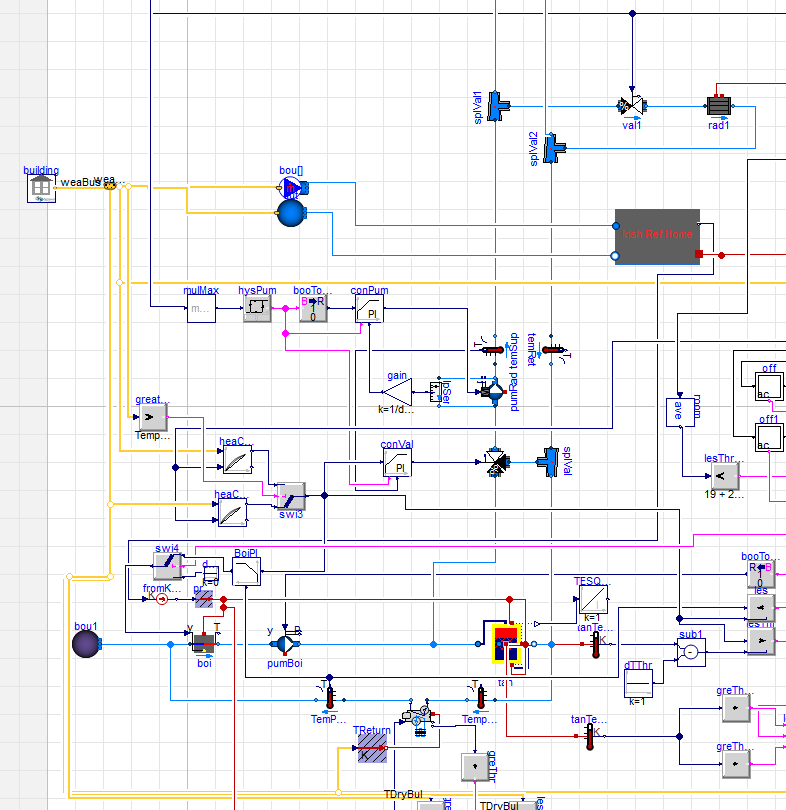
\includegraphics[width=0.9\linewidth]{boilerandHP}
    \caption{Boiler and \acs{HP} section of the \texttt{Modelica} model}
    \label{fig:boilerandhp}
\end{figure}

In \cref{fig:controllersec}, just north of the centre is the day-night setback control section. The \texttt{TRooSet} and \texttt{TRooNig} constant integer outputs are switched by the \texttt{occSch} and \texttt{swi1} blocks. This feeds into the supply temperature demand block. In the centre of the figure is the state machine portion of the control system, comprised of the various \texttt{pumOn} step blocks and \texttt{T1}, \texttt{T2}, etc. transition blocks. The top loop control the boiler and the bottom one controls the \HP. The \texttt{stateGraphRoot} block on the right is necessary for \texttt{Modelica} to keep track of the state machine. There are many \texttt{and} and \texttt{or} blocks connected to the inputs and outputs of the \texttt{Modelica.StateGraph.StepWithSignal} blocks. In the bottom centre two blocks connected by yellow lines can be seen, these are the inequality blocks to test for the outdoor temperature to block the boiler or \HP by blocking the \texttt{T3} and \texttt{T5} respectively. The \texttt{room} \texttt{Buildings.Utilities.Math.Average} block takes the temperatures of all conditioned rooms as a vector and calculates the average, and allows the \texttt{T1} and \texttt{T8} transition blocks to be unblocked if the \texttt{lesThr} block is outputting true. This block is testing whether the temperature at the top of the buffer tank is less than the demanded supply temperature. 
\begin{figure}[htb]
    \centering
    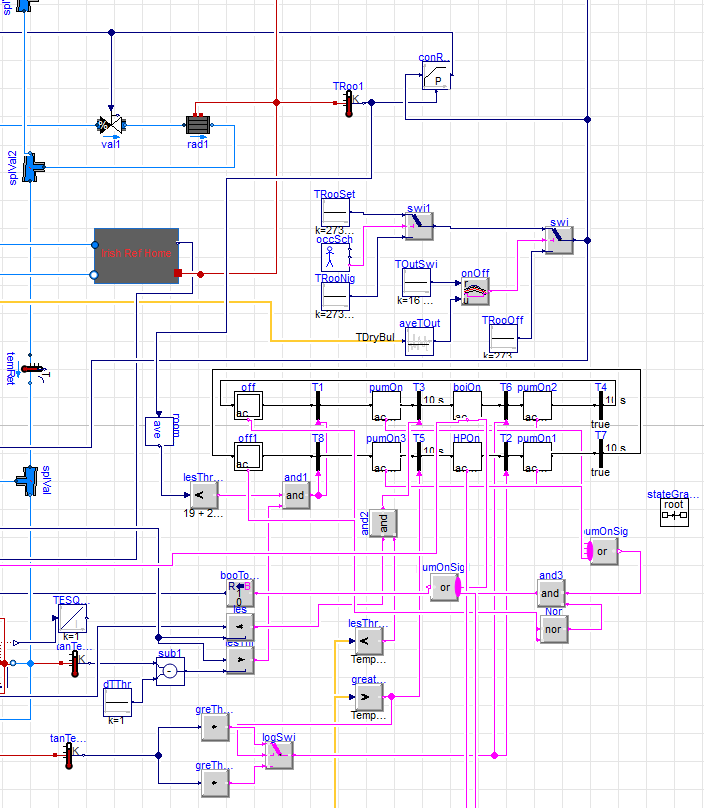
\includegraphics[width=0.9\linewidth]{controller}
    \caption{Controller section of the \texttt{Modelica} model}
    \label{fig:controllersec}
\end{figure}

\cref{fig:frostingmodelsec} shows the frosting model diagram. The \texttt{greThr} block tests whether the \HP is on, and the \texttt{lesThr1} block tests whether it outdoor temperature is less than \qty{2}{\celsius}, the output of these is put into the \texttt{and4} logical and block and passed to the \texttt{accTim} time accumulating block. It is reset if the \texttt{greThr1} block activates the threshold of the \texttt{tim} timer block after a five-minute contiguous period with $T_\text{ext}>\qty{4}{\celsius}$. The \texttt{truHol} block serves as the blocking mechanism of the \HP for a ten-minute period. The second pump and boiler models are to imitate the boiler acting in reverse, the energy usage of the \texttt{boi1} model is summed with the primary boiler model to account for the energy loss due to defrosting. 
\begin{figure}[htb]
    \centering
    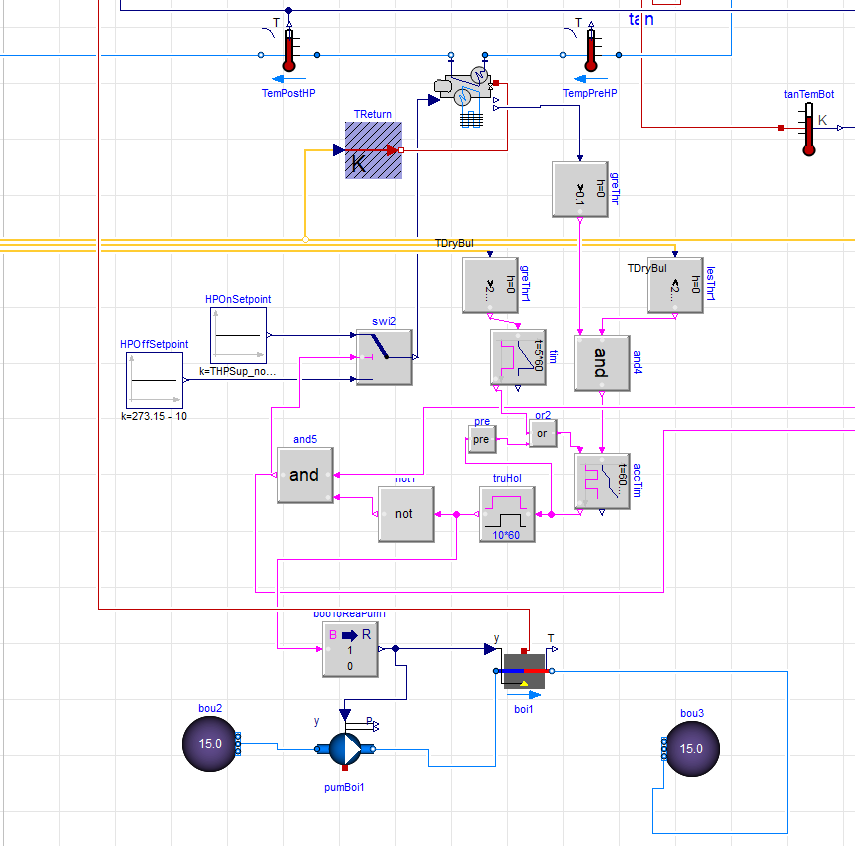
\includegraphics[width=0.9\linewidth]{frosting}
    \caption{Frosting model section of the \texttt{Modelica} model}
    \label{fig:frostingmodelsec}
\end{figure}

\cref{fig:radssec} shows the radiator section of the model. Not all of the connections are rendered as they were not created using the \texttt{Dymola} interface, rather, they were manually created in the underlying code in order to avoid mistakes. The \texttt{rad1}, \texttt{rad2}, etc. blocks are the radiator blocks, as described in \cref{subsec:rad}, serving each of the twelve conditioned rooms, with \texttt{rad3} omitted as the third indexed room is unconditioned. The \texttt{val1}, \texttt{val2}, etc. blocks are controllable valves, limiting the flowrate as a function of the respective volume of the room to the total room volume, and are controlled by the \texttt{conRoo1}, \texttt{conRoo2}, etc. P-controller blocks. The P-controllers take the respective temperature of the room as input via \texttt{TRoo1}, \texttt{TRoo2}, etc. and the \texttt{swi} block from the day-night setback switch. The output of these P-controllers feeds into the \texttt{mulMax} block from \cref{fig:boilerandhp}.
\begin{figure}[htb]
    \centering
    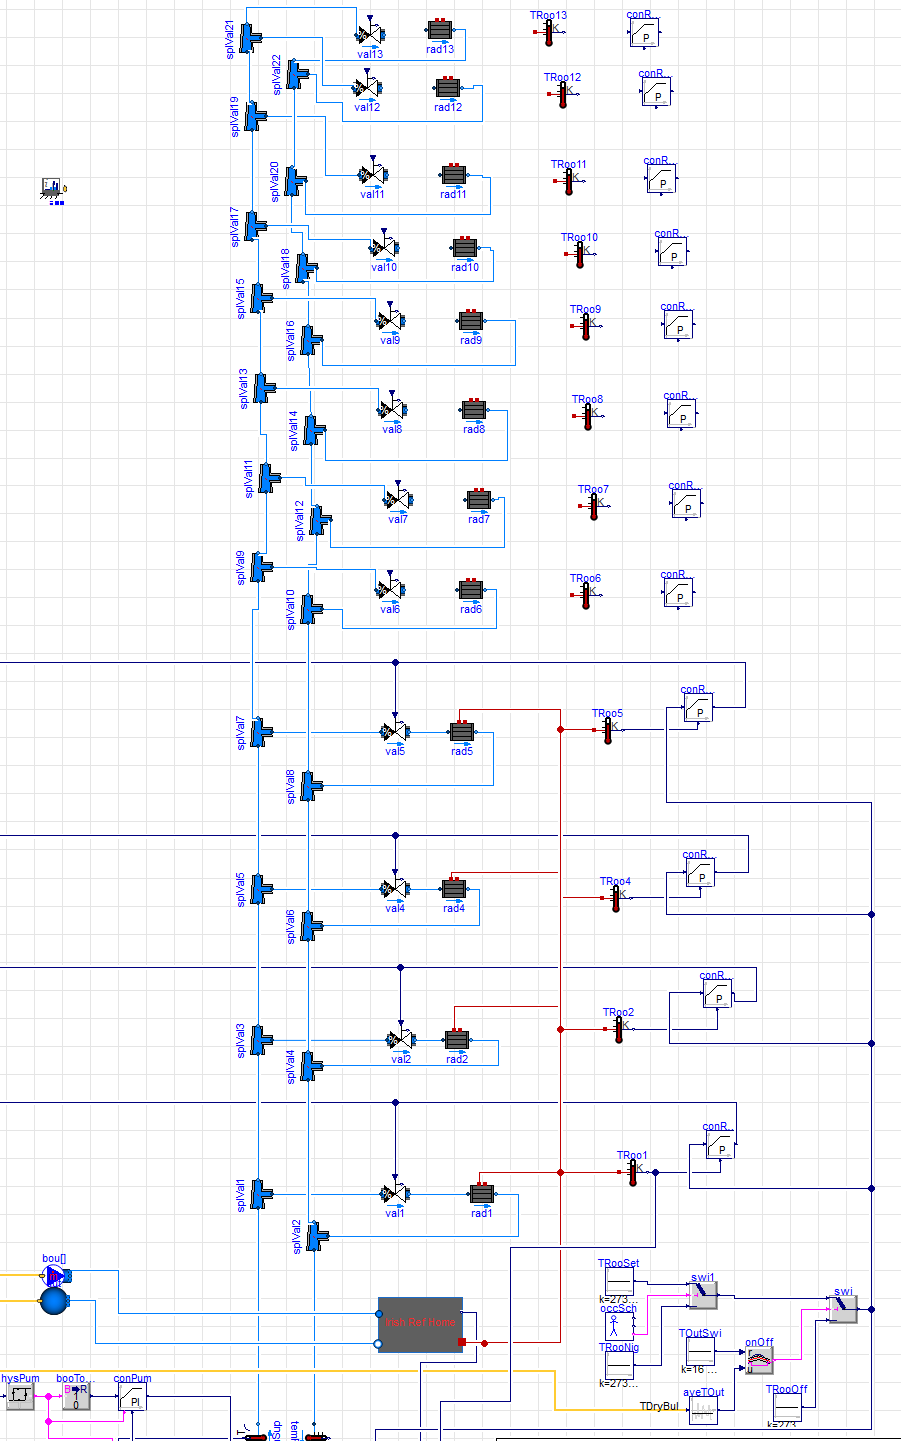
\includegraphics[width=0.85\linewidth]{rads}
    \caption{Radiator section of the \texttt{Modelica} model}
    \label{fig:radssec}
\end{figure}
%********************************************************************
% Other Stuff in the Back
%*******************************************************
\bookmarksetup{startatroot}
\backmatter
%\cleardoublepage\pagestyle{empty}

\hfill

\vfill


\pdfbookmark[-1]{Colophon}{colophon}
\section*{Colophon}
This document was typeset using the typographical look-and-feel \texttt{classicthesis} developed by Andr\'e Miede and Ivo Pletikosić.
The style was inspired by Robert Bringhurst's seminal book on typography ``\emph{The Elements of Typographic Style}''.
\texttt{classicthesis} is available for both \LaTeX\ and \mLyX:
\begin{center}
\url{https://bitbucket.org/amiede/classicthesis/}
\end{center}
Happy users of \texttt{classicthesis} usually send a real postcard to the author, a collection of postcards received so far is featured here:
\begin{center}
\url{http://postcards.miede.de/}
\end{center}
Thank you very much for your feedback and contribution.

\bigskip

\noindent\finalVersionString

%Hermann Zapf's \emph{Palatino} and \emph{Euler} type faces (Type~1 PostScript fonts \emph{URW
%Palladio L} and \emph{FPL}) are used. The ``typewriter'' text is typeset in \emph{Bera Mono},
%originally developed by Bitstream, Inc. as ``Bitstream Vera''. (Type~1 PostScript fonts were made
%available by Malte Rosenau and
%Ulrich Dirr.)

%\paragraph{note:} The custom size of the textblock was calculated
%using the directions given by Mr. Bringhurst (pages 26--29 and
%175/176). 10~pt Palatino needs  133.21~pt for the string
%``abcdefghijklmnopqrstuvwxyz''. This yields a good line length between
%24--26~pc (288--312~pt). Using a ``\emph{double square textblock}''
%with a 1:2 ratio this results in a textblock of 312:624~pt (which
%includes the headline in this design). A good alternative would be the
%``\emph{golden section textblock}'' with a ratio of 1:1.62, here
%312:505.44~pt. For comparison, \texttt{DIV9} of the \texttt{typearea}
%package results in a line length of 389~pt (32.4~pc), which is by far
%too long. However, this information will only be of interest for
%hardcore pseudo-typographers like me.%
%
%To make your own calculations, use the following commands and look up
%the corresponding lengths in the book:
%\begin{verbatim}
%    \settowidth{\abcd}{abcdefghijklmnopqrstuvwxyz}
%    \the\abcd\ % prints the value of the length
%\end{verbatim}
%Please see the file \texttt{classicthesis.sty} for some precalculated
%values for Palatino and Minion.
%
%    \settowidth{\abcd}{abcdefghijklmnopqrstuvwxyz}
%    \the\abcd\ % prints the value of the length

% ********************************************************************
% Game Over: Restore, Restart, or Quit?
%*******************************************************
\end{document}
% ********************************************************************
